\documentclass[a4paper]{amsart}
%\usepackage{a4wide}
\usepackage{fullpage}
\usepackage[pdftex]{graphicx}
\usepackage[pdftex,debug]{hyperref}
\usepackage{amsmath,amssymb,amsthm}
\usepackage{bm}
\usepackage{tikz}
\usepackage{verbatim}

\newcommand{\N}         {{\mathbb{N}}}
\newcommand{\Z}         {{\mathbb{Z}}}
\newcommand{\Q}         {{\mathbb{Q}}}
\newcommand{\R}         {{\mathbb{R}}}
\newcommand{\C}         {{\mathbb{C}}}
\newcommand{\bbm}       {\begin{bmatrix}}
\newcommand{\bsm}       {\left[\begin{smallmatrix}}
\newcommand{\ebm}       {\end{bmatrix}}
\newcommand{\esm}       {\end{smallmatrix}\right]}
\newcommand{\bcf}[2]{\left(\begin{array}{c}{#1}\\{#2}\end{array}\right)}
\newcommand{\tm}        {\times}
\newcommand{\iffa}      {\Leftrightarrow}
\newcommand{\half}      {\tfrac{1}{2}}

\newcommand{\al}        {\alpha}
\newcommand{\bt}        {\beta}
\newcommand{\gm}        {\gamma}
\newcommand{\dl}        {\delta}
\newcommand{\ep}        {\epsilon}
\newcommand{\zt}        {\zeta}
\newcommand{\et}        {\eta}
\newcommand{\tht}       {\theta}
\newcommand{\io}        {\iota}
\newcommand{\kp}        {\kappa}
\newcommand{\lm}        {\lambda}
\newcommand{\ph}        {\phi}
\newcommand{\ch}        {\chi}
\newcommand{\ps}        {\psi}
\newcommand{\rh}        {\rho}
\newcommand{\sg}        {\sigma}
\newcommand{\om}        {\omega}

\newcommand{\vp}        {\mathbf{p}}
\newcommand{\vq}        {\mathbf{q}}
\newcommand{\vr}        {\mathbf{r}}
\newcommand{\Dl}        {\Delta}
\newcommand{\sm}        {\setminus}
\newcommand{\sse}       {\subseteq}
\newcommand{\st}        {\;|\;}
\newcommand{\xra}       {\xrightarrow}

\newcommand{\rr}        {\sqrt{3}}
\newcommand{\rs}        {\sqrt{6}}
\newcommand{\rt}        {\sqrt{2}}

\newcommand{\csch}     {\operatorname{csch}}
\newcommand{\sech}     {\operatorname{sech}}
\newcommand{\arcsinh}  {\operatorname{arcsinh}}
\newcommand{\arccosh}  {\operatorname{arccosh}}
\newcommand{\arctanh}  {\operatorname{arctanh}}

\newcommand{\degree}    {\operatorname{degree}}
\newcommand{\range}     {\operatorname{range}}
\newcommand{\trans}     {\operatorname{trans}}
\newcommand{\trc}       {\operatorname{trace}}
\newcommand{\adj}       {\operatorname{adj}}

\newcommand{\VEC}[1]    {\mathbf{#1}}

\newcommand{\BLUEVIOLET}[1]{#1}
\newcommand{\BLUE}[1]{#1}
\newcommand{\BROWN}[1]{#1}
\newcommand{\CORNFLOWERBLUE}[1]{#1}
\newcommand{\DARKORCHID}[1]{#1}
\newcommand{\EMERALD}[1]{#1}
\newcommand{\GREEN}[1]{#1}
\newcommand{\MAGENTA}[1]{#1}
\newcommand{\MAROON}[1]{#1}
\newcommand{\OLIVEGREEN}[1]{#1}
\newcommand{\ORANGE}[1]{#1}
\newcommand{\PINEGREEN}[1]{#1}
\newcommand{\PURPLE}[1]{#1}
\newcommand{\REDVIOLET}[1]{#1}
\newcommand{\RED}[1]{#1}
\newcommand{\ROYALBLUE}[1]{#1}
\newcommand{\RUBINERED}[1]{#1}
\newcommand{\YELLOWORANGE}[1]{#1}


\newcommand{\EMPH}{\emph}
\newcommand{\DEFN}{\emph}
\newcommand{\PMA}{PMA}
\newcommand{\ghost}{}
\newcommand{\mathworld}[1]{}
\newcommand{\exref}[1]{another exercise}
\renewcommand{\:}{\colon}

\renewcommand{\marks}[1]{}
\newcommand{\mks}[1]{}
\newcommand{\mk}{}


\theoremstyle{definition}

\newtheorem{exercise}{Exercise}[section]
\newenvironment{solution}{{\noindent \bf Solution:}}{}

\title{Problems for Maths with Maple}
\begin{document}

\maketitle

\section*{Week 1}
\addtocounter{section}{1}\setcounter{exercise}{0}

\begin{exercise}\label{ex-lin-misc-i}
Solve the equations
 \begin{align*}
  w+x+y+z &= 1234 & \text{(1)} & &
  w+x-y-z &= 1210 & \text{(2)} \\
  w-x+y-z &= 1010 & \text{(3)} & &
  w-x-y+z &=  990 & \text{(4)}
 \end{align*}
\end{exercise}
\begin{solution}
We deduce further equations as follows:
 \begin{align*}
  2y+2z &= 24  \tag{(5)=(1)-(2)} \\
  2x+2z &= 224 \tag{(6)=(1)-(3)} \\
  2x+2y &= 244 \tag{(7)=(1)-(4)} \\
  2x-2y &= 200 \tag{(8)=(6)-(5)} \\
  4x    &= 444 \tag{(9)=(7)+(8)}
 \end{align*}
 From this we get $x=111$, which we substitute in~(7) and~(6) to get
 $y=11$ and $z=1$.  Putting these in~(1) gives $w=1111$.  In
 conclusion, we have
 \[ (w,x,y,z) = (1111,111,11,1). \]
\end{solution}
\begin{exercise}\label{ex-circ-geom}
As you work through~(a) to~(g) below, draw a diagram showing all the
 curves, points and lines involved.
 \begin{itemize} 
  \item[(a)] Let $C$ be the curve $x^2+y^2=25$.  Describe this
   geometrically.  Note that the points $P=(-5,0)$ and $Q=(3,4)$ lie
   on $C$.
  \item[(b)] Let $L$ be the line joining $P$ to $Q$.  What is the
   equation for $L$?  What is its slope (or in other words, its gradient)? 
  \item[(c)] Let $M$ be the line of slope $-2$ passing through $Q$.
   What is the equation for $M$?  
  \item[(d)] Let $R$ be the point (other than $Q$) where $M$ meets
   $C$.  What are the coordinates of $R$?
  \item[(e)] What is the angle between $L$ and $M$?  (Note: here and almost
   everywhere else in University mathematics, angles are measured in
   radians, not degrees.)  Do you know a general geometric fact that
   explains this?   
  \item[(f)] Let $S$ be the midpoint of the line segment $PQ$.  What
   are the coordinates of $S$?
  \item[(g)] Let $N$ be the line joining $S$ to the origin $O=(0,0)$.
   Show that $N$ is parallel to $M$.
 \end{itemize}
\end{exercise}
\begin{solution}
 \begin{center}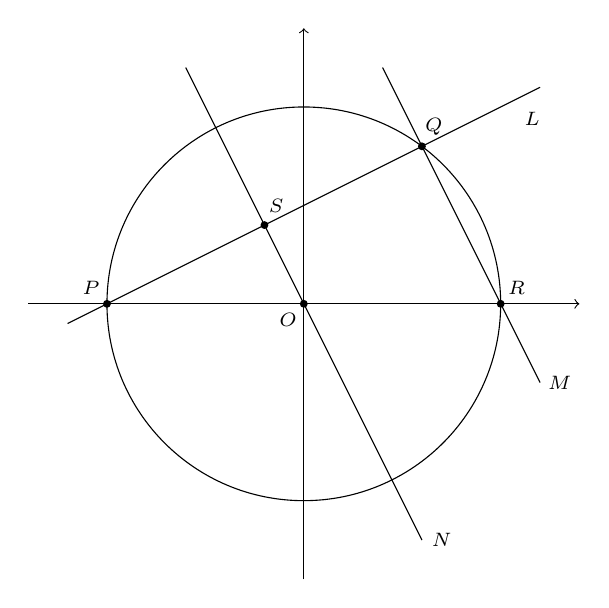
\begin{tikzpicture}[scale=0.5]
  \draw (-6.0,-0.5) -- ( 6.0, 5.5);
  \draw ( 2.0, 6.0) -- ( 6.0,-2.0);
  \draw (-3.0, 6.0) -- ( 3.0,-6.0);
  \draw[->] (-7,0) -- (7,0);
  \draw[->] (0,-7) -- (0,7);
  \draw (0,0) circle(5);
  \fill[black] ( 0, 0) circle(0.1);
  \fill[black] (-5, 0) circle(0.1);
  \fill[black] ( 3, 4) circle(0.1);
  \fill[black] ( 5, 0) circle(0.1);
  \fill[black] (-1, 2) circle(0.1);
  \draw (-0.4,-0.4) node {$\scriptstyle O$};
  \draw (-5.4, 0.4) node {$\scriptstyle P$};
  \draw ( 3.3, 4.5) node {$\scriptstyle Q$};
  \draw ( 5.4, 0.4) node {$\scriptstyle R$};
  \draw (-0.7, 2.5) node {$\scriptstyle S$};
  \draw ( 5.8, 4.7) node {$\scriptstyle L$}; 
  \draw ( 6.5,-2.0) node {$\scriptstyle M$}; 
  \draw ( 3.5,-6.0) node {$\scriptstyle N$}; 
 \end{tikzpicture}\end{center}
 \begin{itemize}
  \item[(a)] $C$ is the circle of radius $5$ centred at the origin.
  \item[(b)] The equation for $L$ is $y=x/2+5/2$, with slope $1/2$.
   (One way to obtain this is to say that the equation must be $y=mx+b$
   for some $m$ and $b$.  As $P=(-5,0)$ lies on the line, we must have
   $0=-5m+b$, so $b=5m$.  As $Q=(3,4)$ lies on the line, we must
   $4=3m+b=3m+5m=8m$, so $m=1/2$, so $b=5/2$.)
  \item[(c)] The equation for $M$ is $y-4=-2(x-3)$, or equivalently
   $y=-2x+10$. 
  \item[(d)] $M$ meets $C$ at the points $(x,y)$ where $y=-2x+10$
   and $x^2+y^2=25$, which implies $x^2+(-2x+10)^2=25$.  This can be
   expanded and rearranged as $5x^2-40x+75=0$, or $5(x-3)(x-5)=0$, so
   $x=3$ or $x=5$.  Using $y=-2x+10$ we see that the intersection
   points are $(3,4)$ and $(5,0)$.  The first of these is $Q$, so $R$
   must be $(5,0)$.
  \item[(e)] The slope of $L$ times the slope of $M$ is
   $(1/2).(-2)=-1$, which means that $L$ and $M$ are at right angles
   to each other.  In fact, whenever you have a triangle with one side
   being the diameter of a circle and the third vertex also lying on
   the circle, then the angle at the third vertex is always a right
   angle (often stated as ``the angle in a semicircle is a right
   angle''). 
  \item[(f)] The point $S$ is $(P+Q)/2=(-5+3,0+4)/2=(-1,2)$.  The line
   $N$ joining $S$ to $O$ is $y=-2x$, with slope $-2$.  This is the
   same as the slope of $M$, so $N$ and $M$ are parallel.
 \end{itemize}
\end{solution}
\begin{exercise}\label{ex-diff-misc-i}
Differentiate the following functions, simplifying your
 answers as much as possible:
 \[
  \text{\textbf{(a)}}\quad x+x^{10}+x^{100} \hspace{2em}
  \text{\textbf{(b)}}\quad (3x+2)/(4x+3) \hspace{2em} 
  \text{\textbf{(c)}}\quad x\log(x)-x \hspace{2em}
  \text{\textbf{(d)}}\quad e^{-x}\sin(10 x) \hspace{2em}
  \text{\textbf{(e)}}\quad \sin(x^2)
 \]
\end{exercise}
\begin{solution}
\begin{itemize}
  \item[(a)] Using the rule $\tfrac{d}{dx}(x^n)=n\,x^{n-1}$ we find
    that the derivative is $1+10x^9+100x^{99}$
  \item[(b)] Here we use the quotient rule 
   \[ \tfrac{d}{dx}\left(\tfrac{u}{v}\right) =
       \left(\tfrac{du}{dx}v - u\tfrac{dv}{dx}\right)/v^2.
   \]
   We have $u=3x+2$ and $v=4x+3$, so $du/dx=3$ and $dv/dx=4$, so
   $\tfrac{du}{dx}v-u\tfrac{dv}{dx}=3(4x+3)-4(3x+2)=1$.  The
   derivative is thus $1/(4x+3)^2$
  \item[(c)] We differentiate $x\log(x)$ using the product rule
    $\tfrac{d}{dx}(uv)=\tfrac{du}{dx}v+u\tfrac{dv}{dx}$, and
    remembering that $\tfrac{d}{dx}\log(x)=1/x$.  This gives
    $\tfrac{d}{dx}(x\log(x))=1.\log(x)+x.1/x=\log(x)+1$.  As
    $\tfrac{d}{dx}x=1$ this gives
    $\tfrac{d}{dx}(x\log(x)-x)=\log(x)+1-1=\log(x)$. 
  \item[(d)] We use the product rule again, together with the facts
    that $\frac{d}{dx}e^{-x}=-e^{-x}$ and
    $\frac{d}{dx}\sin(10x)=10\cos(10x)$.  We find that the final
    answer is $e^{-x}(10\cos(10 x)-\sin(10 x))$.
  \item[(e)] Write $u=x^2$ and $y=\sin(u)=\sin(x^2)$.  We are asked to
    find $dy/dx$, but the chain rule tells us that this is the same as
    $\frac{dy}{du}\,\frac{du}{dx}$.  Here $y=\sin(u)$ so
    $dy/du=\cos(u)=\cos(x^2)$, and $du/dx=2x$, so $dy/dx=2x\cos(x^2)$.
 \end{itemize}
\end{solution}
\begin{exercise}\label{ex-int-misc-i}
Evaluate the following integrals:
\[ 
  \text{\textbf{(a)}}\quad \int x^9+x^{99}+x^{999}\,dx \hspace{1em}
  \text{\textbf{(b)}}\quad \displaystyle\int x\,e^{3x}\,dx \hspace{1em}
  \text{\textbf{(c)}}\quad \displaystyle\int x\,e^{-x^2}\,dx \hspace{1em}
  \text{\textbf{(d)}}\quad \displaystyle\int\frac{dx}{\sqrt{1-x^2}} \hspace{1em}
  \text{\textbf{(e)}}\quad \displaystyle\int_1^{e^2}\frac{dx}{x}
\]
\end{exercise}
\begin{solution}
\begin{itemize}
  \item[(a)] Using the rule $\int x^n\,dx=x^{n+1}/(n+1)$ we find that
    the integral is 
    $\displaystyle
      \frac{x^{10}}{10}+\frac{x^{100}}{100}+\frac{x^{1000}}{1000}$.
  \item[(b)] Here we integrate by parts, taking $u=x$ and
    $dv/dx=e^{3x}$, so that $du/dx=1$ and $v=e^{3x}/3$.  This gives 
    \[ \int x\,e^{3x}\,dx = \tfrac{1}{3}x\,e^{3x} - 
        \int \tfrac{1}{3}e^{3x}\,dx = 
        \tfrac{1}{3}x\,e^{3x} - \tfrac{1}{9}e^{3x} = 
        (x/3-1/9)e^{3x}.
    \] 
  \item[(c)] Here we substitute $u=-x^2$, so $du=-2x\,dx$ or
    equivalently $dx=-du/(2x)$.  This gives
    \[ \int x\,e^{-x^2}\,dx = 
        \int x\,e^u\,\frac{-du}{2x} = 
        -\frac{1}{2}\int e^u\, du = 
        -\frac{1}{2}e^u = -e^{-x^2}/2.
    \]
  \item[(d)] Here we substitute $x=\sin(t)$, so $dx=\cos(t)\,dt$.  As
    $\sin(t)^2+\cos(t)^2=1$ we have $\sqrt{1-x^2}=\cos(t)$.  It
    follows that 
    \[ \int\frac{dx}{\sqrt{1-x^2}} = \int\frac{\cos(t)\,dt}{\cos(t)}
        = \int 1\,dt = t = \arcsin(x).
    \]
  \item[(e)] It is standard that $\int\frac{dx}{x}=\log(x)$, so
    $\int_1^{e^2}\frac{dx}{x}=\log(e^2)-\log(1)=2-0=2$.
 \end{itemize}
\end{solution}

\begin{exercise}\label{ex-giga}
We have $10^3=1000\approx 1024=2^{10}$.  Deduce similar
 approximations for $10^9$ and $8\tm 10^9$ as powers of $2$.
\end{exercise}
\begin{solution}
\begin{align*}
  10^9 &=10^{3\tm 3}=(10^3)^3\approx(2^{10})^3=2^{10\tm 3}=2^{30}\\
  8\tm 10^9 &= 2^3\tm 10^9\simeq 2^3\tm 2^{30} = 2^{33}.
 \end{align*}
 (The exact numbers are $2^{30}=1073741824$ and $2^{33}=8589934592$.)

 According to the usual metric conventions, a ``gigabyte'' of memory
 should contain $10^9$ bytes.  Because digital electronics is based on
 binary numbers, it is easier and more natural to build memory chips
 with $2^{30}$ bytes of capacity, so that is what a gigabyte means in
 practice.  A byte is $8$ bits, so the capacity is
 $8\tm 2^{30}=2^{33}\approx 8\tm 10^9$ bits.
\end{solution}

\begin{exercise}\label{ex-seventh}
\begin{itemize}
  \item[(a)] Give a formula for the infinite sum
   $S=\sum_{i=0}^\infty x^i=1+x+x^2+\dotsb$.  (You may assume that
   $|x|<1$.) 
  \item[(b)] Deduce a formula for the infinite sum
   $T=\sum_{i=1}^\infty x^i=x+x^2+x^3+\dotsb$.
  \item[(c)] Consider the expression
   \[ y = 142857 (10^{-6} + 10^{-12} + 10^{-18} + \dotsb). \]
   Write the terms $142857\tm 10^{-6}$, $142857\tm 10^{-12}$ and 
   $142857\tm 10^{-18}$ as decimals.  What is the decimal expansion of
   $y$ itself?
  \item[(d)] Using part~(b), give an exact expression for $1/y$.
   (Your answer should be a whole number, not a fraction.)
 \end{itemize}
\end{exercise}

\begin{solution}
\begin{itemize}
  \item[(a)] The geometric progression formula says that 
   $S=1/(1-x)$.  (The proof is as follows: note that
   $xS=x(1+x+x^2+\dotsb)=x+x^2+x^3+\dotsb=S-1$.  Rearranging this gives
   $(1-x)S=1$ and so $S=1/(1-x)$.)
  \item[(b)] From the defining formulae we see that $T=xS=x/(1-x)$.
   Alternatively, we see from the formulae that $T=S-1=1/(x-1)-1$, but
   this can be simplified to $x/(1-x)$ again.
  \item[(c)]
   We have
   \begin{align*}
    142857 \tm 10^{-6}  &= 0.142857 \\
    142857 \tm 10^{-12} &= 0.000000142857 \\
    142857 \tm 10^{-18} &= 0.000000000000142857
   \end{align*}
   By adding these together with all the subsequent terms in the
   sequence, we see that $y$ is the recurring decimal
   \[ 0.142857142857142857142857\ldots = 0.\dot{1}4285\dot{7}. \] 
  \item[(d)] Part~(b) (with $x=10^{-6}$) tells us that
   \begin{align*}
    10^{-6} + 10^{-12} + 10^{-18} + \dotsb 
     &= 10^{-6} + (10^{-6})^2 + (10^{-6})^3 + \dotsb \\
     &= 10^{-6}/(1-10^{-6}) = 1/(10^6-1) = 1/999999.
   \end{align*}
   This gives $y=142857/999999$ and so
   \[ y^{-1} = \left(\frac{142857}{999999}\right)^{-1}
        = \frac{999999}{142857} = 7.
   \]
   Putting all this together, we conclude that
   $1/7=0.\dot{1}4285\dot{7}$. 
 \end{itemize}
\end{solution}

\begin{exercise}\label{ex-expand-cyclotomic}
Consider the following functions:
 \[ \begin{array}{rclcrcl}
  \phi_1(x) &=& x - 1 & \hspace{4em} &
   \phi_5(x) &=& x^4 + x^3 + x^2 + x + 1\\
  \phi_2(x) &=& x + 1 &&
   \phi_6(x) &=& x^2 - x + 1\\
  \phi_3(x) &=& x^2 + x + 1 &&
   \phi_{12}(x) &=& x^4 - x^2 + 1 \\
  \phi_4(x) &=& x^2 + 1
 \end{array} \]
 (These are called \emph{cyclotomic polynomials}.  They are
 very important in \emph{Number Theory}, which means the
 study of prime numbers, divisibility and so on.)

 Expand out the following products:
 \[ 
   \phi_1(x)\phi_2(x) \hspace{2em}
   \phi_1(x)\phi_3(x) \hspace{2em}
   \phi_1(x)\phi_2(x)\phi_4(x) \hspace{2em}
   \phi_1(x)\phi_5(x) \hspace{2em}
   \phi_1(x)\phi_2(x)\phi_3(x)\phi_6(x).
 \]
 Can you see the pattern?  Can you guess what is the corresponding
 equation involving $\phi_{12}(x)$?
\end{exercise}
\begin{solution}
\begin{align*}
  \phi_1(x)\phi_2(x) &= (x-1)(x+1) = x^2 - 1 \\
  \phi_1(x)\phi_3(x) &= (x-1)(x^2+x+1) = x^3 - 1 \\
  \phi_1(x)\phi_2(x)\phi_4(x) &= (x-1)(x+1)(x^2+1) \\
                              &= (x^2-1)(x^2+1) = x^4 - 1 \\
  \phi_1(x)\phi_5(x) &= (x-1)(x^4+x^3+x^2+x+1) = x^5 - 1 \\
  \phi_1(x)\phi_2(x)\phi_3(x)\phi_6(x)
   &= (x-1)(x+1)(x^2+x+1)(x^2-x+1) \\
   &= (x^2-1)(x^4+x^2+1) = x^6 - 1.
 \end{align*}
 The general rule so far is as follows: for any number $n$, we take
 all the numbers $d$ that divide $n$, take the corresponding
 polynomials $\phi_d(x)$, multiply them together, and we get $x^n-1$.
 (Consider the case $n=6$, for example: the divisors of $6$ are $1$,
 $2$, $3$ and $6$, the corresponding polynomials are $\phi_1(x)$,
 $\phi_2(x)$, $\phi_3(x)$ and $\phi_6(x)$, and we saw above that if we
 multiply these together, we get $x^6-1$.)  This suggests that we
 should have
 \[ \phi_1(x)\phi_2(x)\phi_3(x)\phi_4(x)\phi_6(x)\phi_{12}(x) =
     x^{12} - 1.
 \]
 If we feed in the case $n=6$ which we have already worked out, the
 left hand side becomes $(x^6-1)\phi_4(x)\phi_{12}(x)$.  It is easy to
 check that $\phi_4(x)\phi_{12}(x)=x^6+1$, so the left hand side
 becomes $(x^6-1)(x^6+1)$ which is $x^{12}-1$ as expected.
\end{solution}

\begin{exercise}\label{ex-discrete-derivative}
Put
 \begin{align*}
  b_3(x) &= x(x-1)(x-2)/6 \\
  b_4(x) &= x(x-1)(x-2)(x-3)/24 \\
  b_5(x) &= x(x-1)(x-2)(x-3)(x-4)/120.
 \end{align*}
 \begin{itemize}
  \item Simplify $b_4(x+1)-b_4(x)$.  If you do this in the right way,
   it will take only a few simple steps; if you do it the wrong way,
   you will have to work much harder.  Do not expand anything out if
   you do not have to.
  \item Simplify $b_5(x+1)-b_5(x)$.
  \item What is the general pattern?  (Your answer should include a 
   definition of $b_n(x)$ for all $n$.)
 \end{itemize}
\end{exercise}
\begin{solution}
We have
 \begin{align*}
  b_4(x+1) &= (x+1)(x+1-1)(x+1-2)(x+1-3)/24 \\
           &= {(x+1)}{x(x-1)(x-2)}/24 \\
  b_4(x)   &= {x(x-1)(x-2)}{(x-3)}/24, \\
  \intertext{so}
  b_4(x+1)-b_4(x) &= 
   ({(x+1)}-{(x-3)}){x(x-1)(x-2)}/24 \\
  &= 4{x(x-1)(x-2)}/24 \\
  &= x(x-1)(x-2)/6 = b_3(x).
 \end{align*}
 Similarly,
 \begin{align*}
  b_5(x+1) &= {(x+1)}{x(x-1)(x-2)(x-3)}/120 \\
  b_5(x)   &= {x(x-1)(x-2)(x-3)}{(x-4)}/120, \\
  \intertext{so}
  b_5(x+1)-b_5(x) &= 
   ({(x+1)}-{(x-4)}){x(x-1)(x-2)(x-3)}/120 \\
  &= {x(x-1)(x-2)(x-3)}/24 = b_4(x).
 \end{align*}
 The general pattern is that $b_n(x+1)-b_n(x)=b_{n-1}(x)$, where
 \[ b_n(x) = x(x-1)\ldots(x-n+1)/n!. \]
\end{solution}

\section*{Week 2}
\addtocounter{section}{1}\setcounter{exercise}{0}

\begin{exercise}\label{ex-cubic-comp}
Solve the equation
 \[ (((x^3+1)^3+1)^3+1)^3+1=9, \]
 where $x$ is a real number.  (It is not helpful to expand
 out the left hand side.)
\end{exercise}
\begin{solution}
\begin{align*}
   &\hspace{1.7em} (((x^3+1)^3+1)^3+1)^3+1=9 \\
   &\iffa (((x^3+1)^3+1)^3+1)^3=8 \\
   &\iffa ((x^3+1)^3+1)^3+1=8^{1/3}=2 \\
   &\iffa ((x^3+1)^3+1)^3=1 \\
   &\iffa (x^3+1)^3+1=1^{1/3}=1 \\
   &\iffa (x^3+1)^3=0 \\
   &\iffa x^3+1=0 \iffa x^3=-1 \iffa x=-1.
 \end{align*}
 Thus, the only solution is $x=-1$.  Another way to write this is to
 use the function $f(t)=t^3+1$ and the inverse function
 $f^{-1}(s)=(s-1)^{1/3}$.  The given equation says $f(f(f(f(x))))=9$,
 and the solution is $x=f^{-1}(f^{-1}(f^{-1}(f^{-1}(9))))$.  We have
 $f^{-1}(9)=2$ and $f^{-1}(2)=1$ and $f^{-1}(1)=0$ and $f^{-1}(0)=-1$,
 so the conclusion is that $x=-1$.

 If you ask Maple to do this problem, it will think for a
 while and then report a long list of 81 solutions.  In fact,
 some of these solutions are mentioned more than once, so
 there are only 75 different solutions.  Moreover, 74 of
 them are complex numbers and so are not allowed in this
 question.  The only real solution is $x=-1$.
\end{solution}
\begin{exercise}\label{ex-cubic-log}
Solve the equation $\ln(x)^3=\ln(x)$.
\end{exercise}
\begin{solution}
 \begin{align*}
         & \ln(x)^3 = \ln(x) \\
   \iffa & \ln(x)^3 - \ln(x) = 0 \\
   \iffa & \ln(x)(\ln(x)-1)(\ln(x)+1) = 0 \\
   \iffa & \ln(x) \in \{0,1,-1\}  \\
   \iffa & x \in \{1,e,e^{-1}\}.
 \end{align*}
\end{solution}
\begin{exercise}\label{ex-quad-cos}
Find a solution to the equation $\cos(\tht)^2+2\cos(\tht)=3$ where
 $\tht$ is a real number and $\tht>10$.
\end{exercise}
\begin{solution}
We first rearrange as $\cos(\tht)^2+2\cos(\tht)-3=0$, which factors
 as $(\cos(\tht)-1)(\cos(\tht)+3)=0$.  As $\cos(\tht)$ only ranges
 between $-1$ and $+1$, the factor $\cos(\tht)+3$ is never zero, so we
 must instead have $\cos(\tht)-1=0$, so $\cos(\tht)=1$.  This means
 that $\tht=2n\pi$ for some integer $n$.  Note that $2\pi\simeq 6.28$
 and $4\pi\simeq 12.56$.  Thus, for $\tht>10$, we must have $n\geq 2$.
 The smallest possible answer is thus $\tht=4\pi$.
\end{solution}
\begin{exercise}\label{ex-log-linear}
 You are given that $x,y>0$ and that 
 \[ (A)\qquad x^3y^2 = e \hspace{6em}
    (B)\qquad x^4y^3 = e^2.
 \]
 Find $x$ and $y$.  (One method is to take logs.)
\end{exercise}
\begin{solution}
If we take the log of both sides of the equation $x^3y^2=e$, we get
 $\ln(x^3y^2)=\ln(e)$, or equivalently $3\ln(x)+2\ln(y)=1$.  Treating
 the other equation similarly, we have
 \begin{align*}
  3\ln(x) + 2\ln(y) &= 1 &\hspace{1em}& (\ln(A)) \\
  4\ln(x) + 3\ln(y) &= 2 &\hspace{1em}& (\ln(B))
 \intertext{These equations can be solved for $\ln(x)$ and $\ln(y)$:}
  \ln(x) &= -1 &\hspace{1em}& (3\ln(A)-2\ln(B)) \\
  \ln(y) &= 2  &\hspace{1em}& (3\ln(B)-4\ln(A))
 \end{align*}
 This gives $x=e^{-1}$ and $y=e^2$.

 For an alternative approach, we can divide the cube of equation~(A)
 by the square of equation~(B):
 \begin{align*}
  x^9y^6 &= e^3 &\hspace{1em}& (A^3) \\
  x^8y^6 &= e^4 &\hspace{1em}& (B^2) \\
  x &= e^{-1}   &\hspace{1em}& (A^3/B^2).
 \end{align*}
 We can substitute this back into equation~(A) to get $y^2=e^4$ and so
 $y=e^2$ again.
\end{solution}
\begin{exercise}\label{ex-log-cubic}
Solve the equation $\ln(e^{3t}-7)=0$.
\end{exercise}
\begin{solution}
 Start with the given equation $\ln(e^{3t}-7)=0$.  We can take the
 exponential of both sides to get $e^{\ln(e^{3t}-7)}=e^0=1$.  Using
 the rule $e^{\ln(x)}=x$ we can simplify the left hand side to
 $e^{3t}-7$, so $e^{3t}-7=1$, so $e^{3t}=8$.  We can now take the
 logarithm of both sides to give $3t=\ln(8)$, or equivalently
 $t=\ln(8)/3$.  This can be simplified further if we note that
 $8=2^3$, so $\ln(8)=3\ln(2)$; this gives $t=\ln(2)$.

 Note that the rule $\ln(a-b)=\ln(a)-\ln(b)$ is \textbf{not} valid, so
 we \textbf{cannot} start by converting $\ln(e^{3t}-7)$ to
 $\ln(e^{3t})-\ln(7)$. 
\end{solution}

\begin{exercise}\label{ex-log-shift}
Solve the equation $\ln(e^x+1)=x+1$.
\end{exercise}
\begin{solution}
 Start with the given equation $\ln(e^x+1)=x+1$.  We can take the
 exponential of both sides to get $e^{\ln(e^x+1)}=e^{x+1}$.  We can
 use the rule $e^{\ln(a)}=a$ to simplify the left hand side to
 $e^x+1$.  We can use the rules $e^{a+b}=e^ae^b$ and $e^1=e$ to
 simplify the right hand side to $e^xe$.  We now have $e^x+1=e^xe$,
 which can be rearranged as $e^x(e-1)=1$, so $e^x=1/(e-1)$.  We now
 take logs on both sides to get $x=\ln(1/(e-1))=-\ln(e-1)$.

 Note that the rule $\ln(a+b)=\ln(a)+\ln(b)$ is \textbf{not} valid, so
 we \textbf{cannot} start by converting $\ln(e^x+1)$ to
 $\ln(e^x)+\ln(1)$. 
\end{solution}

\begin{exercise}\label{ex-helix-sphere}
Solve the following equations:
 \[
  x = \sin(t) \hspace{4em}
  y = \cos(t) \hspace{4em}
  z = 6t/\pi  \hspace{4em}
  x^2+y^2+z^2 = 10.
 \]
 (In physics, this determines the time and place where an electron
 moving in a magnetic field hits the wall of a spherical chamber.)
\end{exercise}
\begin{solution}
We have $x^2+y^2=\sin(t)^2+\cos(t)^2=1$, so the last equation
 simplifies to $z^2=9$, giving $z=\pm 3$.  The third equation
 rearranges to give $t=\pi z/6=\pm \pi/2$.  It follows in turn that
 $x=\sin(\pm\pi/2)=\pm 1$ and $y=\cos(\pm\pi/2)=0$.  Thus, the two
 possible solutions are $(x,y,z,t)=(1,0,3,\pi/2)$ and
 $(x,y,z,t)=(-1,0,-3,-\pi/2)$.
\end{solution}
\begin{exercise}\label{ex-circ-tangent}
 Given a constant $a>1$, solve the following equations:
 \[ x^2+y^2 = 1 \hspace{6em} (a-x)x - y^2 = 0. \]
 If $x$ and $y$ satisfy the equations, what is $\sqrt{(a-x)^2+y^2}$?

 (Let $C$ be the circle of radius one centred at the origin, and let
 $L$ be one of the two lines through $(a,0)$ that just touches $C$;
 then $L$ meets $C$ at $(x,y)$, where $x$ and $y$ satisfy the
 equations above.)
\end{exercise}
\begin{solution}
 The second equation can be rearranged to give $ax=x^2+y^2$, so
 $ax=1$, so $x=a^{-1}$.  The first equation then gives
 $y=\sqrt{1-x^2}=\sqrt{1-a^{-2}}$.  (We are given that $a>1$, so
 $a^{-2}<1$, so $1-a^{-2}$ is positive and we can meaningfully take
 its square root.)  Thus, the two solutions are
 $(x,y)=(a^{-1},\sqrt{1-a^{-2}})$ and
 $(x,y)=(a^{-1},-\sqrt{1-a^{-2}})$.  In either case we have
 \begin{align*}
  (a-x)^2+y^2 &= (a-a^{-1})^2 + 1 - a^{-2} \\
   &= a^2 - 2 + a^{-2} + 1 - a^{-2} = a^2 - 1 \\
  \sqrt{(a-x)^2+y^2} &= \sqrt{a^2-1}.
 \end{align*}
\end{solution}
\begin{exercise}\label{ex-linear-decimal}
 Consider the equations
 \[
   (1) \qquad a + 2b + 3c = 123 \hspace{5em}
   (2) \qquad 2a + 3b +  c = 231 \hspace{5em}
   (3) \qquad 3a +  b + 2c = 312.
 \]
 Can you see a solution just by looking at the equations?  Solve the
 equations by a more systematic method, and so verify that the visible
 solution is the only solution.
\end{exercise}
\begin{solution}
 It is easy to see that if we put $a=100$ and $b=10$ and $c=1$, then
 the equations are satisfied.  For the more systematic approach, form
 the equations $2.(1)-(2)$ and $3.(1)-(3)$:
 \begin{align*}
  b  + 5c &= 15 \tag{4} \\
  5b + 7c &= 57 \tag{5}
 \end{align*}
 Now take $5.(4)-(5)$:
 \begin{align*}
  18 c &= 18 \tag{6}
 \end{align*}
 This gives $c=1$, which we substitute into~(4) to get $b=10$, which
 we substitute into~(1) to get $a=100$.
\end{solution}
\begin{exercise}\label{ex-lin-degen}
Given a constant $a$, consider the following equations for $x$ and $y$:
 \[ (A)\qquad x + ay = 1   \hspace{6em} (B)\qquad ax + y = a^2 \]
 \begin{itemize}
  \item[(i)] Solve the equations.   Try to write your solution in a
   way that makes sense for $a=1$. 
  \item[(ii)] What happens when $a=-1$?  (You should go back to the
   original equations to answer this, rather than starting from your
   solution for the general case.)
  \item[(iii)] What happens when $a=1$?  (First go back to the original
   equations, then compare with what you get by putting $a=1$ in your
   solution to~(i).)
 \end{itemize}
\end{exercise}
\begin{solution}
 \begin{itemize}
  \item[(i)]
   Form the equations $(A)-a(B)$ and $(B)-a(A)$:
   \begin{align*}
    (C)\qquad (1-a^2)x &= 1-a^3 = (1-a)(1+a+a^2) \\
    (D)\qquad (1-a^2)y &= a^2-a = -a(1-a).
   \end{align*}
   Now divide by $1-a^2$, noting that $1-a^2=(1-a)(1+a)$: this gives
   \begin{align*}
    x &= (1-a^3)/(1-a^2) = (1+a+a^2)/(1+a) \\
    y &= (a^2-1)/(1-a^2) = -a/(1+a).
   \end{align*}
   Note that our final answers make sense when $a=1$, but the
   intermediate calculation does not: we divided by $1-a^2$, which is
   not valid when $a=1$.  When $a=-1$, even the final answer does not
   make sense.
  \item[(ii)]
   Putting $a=-1$ in the original equations gives $x-y=1$ and
   $-x+y=1$, which is equivalent to $x-y=-1$.  These equations are
   inconsistent, so there are no solutions.
  \item[(iii)] 
   If we put $a=1$ then both the original equations become $x+y=1$.
   This means that $x$ can take any value, and $y$ is given by $1-x$.
   If we put $a=1$ in our solution to~(i) we get $x=3/2$ and
   $y=1-x=-1/2$; this is only one of the many solutions.
 \end{itemize}
\end{solution}
\begin{exercise}\label{ex-tetra-solve}
The hydrogen atoms in a molecule of methane lie at the
 points $(0,0,1)$, $(a,0,-b)$, $(-c,d,-b)$ and $(-c,-d,-b)$,
 where $a,b,c,d>0$ and the following equations are
 satisfied:
 \[
  (1)\qquad c^2+d^2 = a^2 \hspace{3em}
  (2)\qquad c^2-d^2 = -ac \hspace{3em}
  (3)\qquad a^2+b^2 = 1   \hspace{3em}
  (4)\qquad b^2+b   = ac. 
 \]
 Solve these equations to find $a$, $b$, $c$ and $d$.
 
 (\textbf{Hint:} find an equation involving only $a$ and
 $c$, and put it in the form $\text{(something)}=0$.
 Factorise it, and note that one of the factors is $>0$, so
 the other one must be zero.  This will let you write $c$ in
 terms of $a$, and thus remove $c$ from equation~(4).  You
 can then combine (3) and (4) to get an equation involving
 only $b$.)
\end{exercise}
\begin{solution}
After adding (1) and (2) and rearranging, we get
 $2c^2+ac-a^2=0$, which factors as $(2c-a)(c+a)=0$.  As
 $a,c>0$ we have $c+a>0$ and so $2c-a=0$, so $c=a/2$.  We
 can now subtract (1) and (2) to get $2d^2=a^2+ac=3a^2/2$,
 so $d^2=3a^2/4$ and $d=\sqrt{3}a/2$.  We can now
 rewrite~(4) as $b^2+b=a^2/2$, but~(3) gives $a^2=1-b^2$, so
 $b^2+b=(1-b^2)/2$.  This can be rearranged as
 $3b^2+2b-1=0$, which factors as $(3b-1)(b+1)=0$.  As
 $b+1>0$ we have $3b-1=0$, so $b=1/3$.  Feeding this
 into~(3) gives $a=\sqrt{1-b^2}=2\sqrt{2}/3$, so
 $c=a/2=\sqrt{2}/3$, and
 $d=\sqrt{3}a/2=\sqrt{2/3}=\sqrt{6}/3$.  In conclusion, we
 have
 \[ a = \frac{2\sqrt{2}}{3}  \hspace{2em}
    b = \frac{1}{3}          \hspace{2em}
    c = \frac{\sqrt{2}}{3}   \hspace{2em}
    d = \frac{\sqrt{6}}{3}
 \]
\end{solution}
\begin{exercise}\label{ex-cuboid}
Solve the following equations for $a,b,c$ and $\lm$
 (assuming that all of these are positive):
 \[ bc=\lm a \hspace{2em}
    ac=\lm b \hspace{2em}
    ab=\lm c \hspace{2em}
    a^2+b^2+c^2 = 1 
 \]
 Hence find the quantity $V=8abc$.  (This is the largest
 possible volume for a cuboid contained in a sphere of
 radius one.  The maximising cuboid has sides of length
 $2a$, $2b$ and $2c$.)
\end{exercise}
\begin{solution}
If we multiply the first two equations we get
 $abc^2=\lm^2ab$.  As $a,b>0$ we can divide by $ab$ to get
 $c^2=\lm^2$.  As $\lm,c>0$ it follows that $c=\lm$.
 Similarly, the first and third equations give $b=\lm$, and
 the first and second equations give $a=\lm$.  The last
 equation then gives $3\lm^2=1$, so $\lm=1/\sqrt{3}$.  It
 follows that
 $V=8(1/\sqrt{3})^3=8/(3\sqrt{3})=8\sqrt{3}/9$.
\end{solution}

\section*{Week 3}
\addtocounter{section}{1}\setcounter{exercise}{0}

\begin{exercise}\label{ex-log-calc}
Calculate the following:
 \[ \log_{10}(10000)   \hspace{4em}
    \log_{100}(10000)  \hspace{4em}
    \log_{1000}(10000) \hspace{4em}
    \log_{1/10}(\sqrt{1000})
 \]
\end{exercise}
\begin{solution}
\begin{itemize}
  \item $10000=10^4$, so $\log_{10}(10000)=4$.
  \item $10000=100^2$, so $\log_{100}(10000)=2$.
  \item $10000=10^4=((1000)^{1/3})^4=1000^{4/3}$, so
   $\log_{1000}(10000)=4/3$.
  \item $10000=10^4=((1/10)^{-1})^4=(1/10)^{-4}$, so
   $\log_{1/10}(10000)=-4$.
 \end{itemize}
 These calculations can also be written slightly differently, using
 the identity $\log_a(x)=\ln(x)/\ln(a)$.  For example, in the last
 case we have
 \[ \log_{1/10}(10000) = \frac{\ln(10000)}{\ln(1/10)} 
     = \frac{4\ln(10)}{-\ln(10)} = -4.
 \]
\end{solution}
\begin{exercise}\label{ex-log-props}
Some of the following statements are true, but others are either
 false or not meaningful.  Decide which is which, and explain why.
 For each statement that is false, give an explicit counterexample.
 If there is a straightforward way to correct the statement, then do
 so. 
 \begin{itemize}
  \item[(a)] $\ln(e^x+e^y)=x+y$
  \item[(b)] If $\ln(x)=a$, then $\ln(-x)=-a$
  \item[(c)] $\log_a(b)\log_b(a)=1$
  \item[(d)] $\exp(\ln(x)-\ln(y))=x-y$ 
  \item[(e)] $\ln(\ln(\exp(\exp(x))))=x$
  \item[(f)] $\exp(\sqrt{x})^2=\exp(x)$
 \end{itemize}
\end{exercise}
\begin{solution}
\begin{itemize}
  \item[(a)] This is false.  For example, when $x=y=0$ the left hand
   side is $\ln(e^0+e^0)=\ln(2)$ but the right hand side is $0$.  A
   correct statement along the same lines is that $\ln(e^xe^y)=x+y$.
  \item[(b)] This is not really meaningful, because $\ln(x)$ is only
   defined when $x>0$, so $\ln(x)$ and $\ln(-x)$ are never both
   defined, so we cannot compare them.  (If we allow complex numbers
   then $\ln(x)$ is defined for $x<0$ but the formula is still false,
   despite many new subtleties that we shall not discuss.)
  \item[(c)] This is true, because $\log_a(b)=\ln(b)/\ln(a)$ and
   $\log_b(a)=\ln(a)/\ln(b)$. 
  \item[(d)] This is false.  For example, when $x=y=1$ the left hand
   side is $\exp(0-0)=\exp(0)=1$, whereas the right hand side is
   $1-1=0$.  A true statement along the same lines is that
   $\exp(\ln(x)-\ln(y))=x/y$. 
  \item[(e)] This is true.  For any number $w$, we have
   $\ln(\exp(w))=w$.  Taking $w=\exp(x)$, we see that
   $\ln(\exp(\exp(x)))=\exp(x)$.  Applying $\ln$ to both sides of this
   equation gives $\ln(\ln(\exp(\exp(x))))=\ln(\exp(x))=x$.
  \item[(f)] This is false.  For example, when $x=1$ the left hand
   side is $\exp(1)^2=e^2$, whereas the right hand side is just $e$.
   A correct statement along the same lines is that
   $\exp(x/2)^2=\exp(x)$. 
 \end{itemize}
\end{solution}
\begin{exercise}\label{ex-hyp-signs}
The following statements are false, but they can be corrected by
 changing some of the signs.  Do so.
 \begin{itemize}
  \item[(a)] $\sinh(x)^2+\cosh(x)^2=1$
  \item[(b)] $\cosh(2x)=\cosh(x)^2-\sinh(x)^2$
  \item[(c)] $\sinh(x+y)=-\sinh(x)\cosh(y)-\cosh(x)\sinh(y)$
 \end{itemize}
\end{exercise}
\begin{solution}
The correct versions are as follows:
 \begin{align*}
  -\sinh(x)^2 + \cosh(x)^2 &= 1 \\
  \cosh(2x) &= \cosh(x)^2 + \sinh(x)^2 \\
  \sinh(x+y) &= \sinh(x)\cosh(y)+\cosh(x)\sinh(y)
 \end{align*}
 Indeed, these are equivalent to the following equations, which can
 easily be checked by expanding everything out:
 \begin{align*}
  -(e^x-e^{-x})^2/4 + (e^x+e^{-x})^2/4 &= 1 \\
  (e^{2x}+e^{-2x})/2 &= (e^x-e^{-x})^2/4 + (e^x+e^{-x})^2/4 \\
  (e^{x+y}-e^{-x-y})/2 &= (e^x-e^{-x})(e^y+e^{-y})/4 + 
                          (e^x+e^{-x})(e^y-e^{-y})/4 
 \end{align*}
\end{solution}
\begin{exercise}\label{ex-log-exp}
Simplify the following expressions (using the identities
 $\ln(xy)=\ln(x)+\ln(y)$, $\exp(x)^n=\exp(nx)$ and so on).
 \begin{itemize}
  \item[(a)] $\ln(xy^2z^3)$
  \item[(b)] $\ln(e^{(x^2)} e^{2xy} e^{(y^2)})$
  \item[(c)] $\displaystyle\frac{\ln(a^n)\ln(a^m)}{\ln(a^p)\ln(a^q)}$
  \item[(d)] $\displaystyle\frac{\exp(a+b\ln(t))}{\exp(a-b\ln(t))}$
  \item[(e)] $\displaystyle\frac{\ln(a^n)\ln(b^m)}{\ln(a^m)\ln(b^n)}$
 \end{itemize}
\end{exercise}
\begin{solution}
\begin{itemize}
  \item[(a)]
   \begin{align*}
    \ln(xy^2z^3) &= \ln(x) + \ln(y^2) + \ln(z^3) \\
                  &= \ln(x) + 2\ln(y) + 3\ln(z).
   \end{align*}
   At the first stage we used the rule $\ln(uv)=\ln(u)+\ln(v)$, and
   at the second stage we used the rule $\ln(u^n)=n\ln(u)$.
  \item[(b)]
   \begin{align*}
    \ln(e^{(x^2)} e^{2xy} e^{(y^2)})
     &= \ln(e^{(x^2+2xy+y^2)}) \\
     &= x^2+2xy+y^2 = (x+y)^2.
   \end{align*}
   At the first stage we used the rule $e^ue^v=e^{u+v}$, and at the
   second stage we used the rule $\ln(e^u)=u$.
  \item[(c)]
   \begin{align*}
    \frac{\ln(a^n)\ln(a^m)}{\ln(a^p)\ln(a^q)}
     &= \frac{n\ln(a).m\ln(a)}{p\ln(a).q\ln(a)} \\
     &= \frac{nm\ln(a)^2}{pq\ln(a)^2} = \frac{nm}{pq}.
   \end{align*}
   Here we just used the rule $\ln(u^n)=n\ln(u)$.
  \item[(d)]
   \begin{align*}
    \frac{\exp(a+b\ln(t))}{\exp(a-b\ln(t))}
     &= \exp((a+b\ln(t))-(a-b\ln(t))) \\
     &= \exp(2b\ln(t)) = \exp(\ln(t))^{2b} = t^{2b}.
   \end{align*}
   Here we used the rule $\exp(u)/\exp(v)=\exp(u-v)$, then the rule
   $\exp(pq)=e^{pq}=\exp(p)^q$, then the rule $\exp(\ln(u))=u$.
  \item[(e)]
   \begin{align*}
    \frac{\ln(a^n)\ln(b^m)}{\ln(a^m)\ln(b^n)}
     &= \frac{n\ln(a).m\ln(b)}{m\ln(a).n\ln(b)} \\
     &= \frac{nm\ln(a)\ln(b)}{nm\ln(a)\ln(b)} = 1.
   \end{align*}
 \end{itemize}
\end{solution}
\begin{exercise}\label{ex-hyp-ident}
Check the identities $\cosh(2x)=2\cosh(x)^2-1$ and
 $\sinh(x+y)=\sinh(x)\cosh(y)+\cosh(x)\sinh(y)$.
\end{exercise}
\begin{solution}
First, we put $u=e^x$, so $u^2=e^{2x}$.  We also have
 $\sinh(x)=(u-u^{-1})/2$ and $\cosh(x)=(u+u^{-1})/2$, so
 \begin{align*}
  2\cosh(x)^2-1 &= 2\left(\frac{u+u^{-1}}{2}\right)^2 - 1
    = 2\frac{u^2 + 2 + u^{-2}}{4} - 1 \\
   &= \frac{u^2 + {2} + u^{-2} - {2}}{2} 
    = \frac{u^2+u^{-2}}{2} \\
   &= \frac{e^{2x} + e^{-2x}}{2} = \cosh(2x).
 \end{align*}
 Next, we put $v=e^y$, so $uv=e^{x+y}$.  We also have
 $\sinh(y)=(v-v^{-1})/2$ and $\cosh(y)=(v+v^{-1})/2$, so
 \begin{align*}
  \sinh(x)\cosh(y)+\cosh(x)\sinh(y) &= 
   \frac{u-u^{-1}}{2} \frac{v+v^{-1}}{2} + 
   \frac{u+u^{-1}}{2} \frac{v-v^{-1}}{2} \\
  &= \frac{1}{4}\left(
      uv + {uv^{-1}} - {u^{-1}v} - u^{-1}v^{-1} +
      uv - {uv^{-1}} + {u^{-1}v} - u^{-1}v^{-1}
     \right) \\
  &= \frac{1}{4}(2uv - 2u^{-1}v^{-1}) = \frac{e^{x+y}-e^{-x-y}}{2} \\
  &= \sinh(x+y).
 \end{align*}
\end{solution}
\begin{exercise}\label{ex-hyp-simp}
Simplify the expressions $4\cosh(x)^3-3\cosh(x)$ and
 $\sinh(x)^2\cosh(x)$.
\end{exercise}
\begin{solution}
Put $u=e^x$.  Then
 \begin{align*}
  4\cosh(x)^3-3\cosh(x)
   &= 4\frac{u^3+3u+3u^{-1}+u^{-3}}{8} - 3\frac{u+u^{-1}}{2}
   \\
   &= \frac{u^3+u^{-3}}{2} = \cosh(3x) \\
  \sinh(x)^2\cosh(x)
   &= \frac{(u-u^{-1})^2}{4} \frac{u+u^{-1}}{2} \\
   &= \frac{1}{8}(u^2-2+u^{-2})(u+u^{-1}) 
    = \frac{1}{8}(u^3-2u+u^{-1}+u-2u^{-1}+u^{-3}) \\ 
   &= \frac{u^3+u^{-3}}{8} - \frac{u+u^{-1}}{8} 
    = \cosh(3x)/4 - \cosh(x)/4. 
 \end{align*}
\end{solution}
\begin{exercise}\label{ex-trig-ident}
Using the fact that $\sin(x)=(e^{ix}-e^{-ix})/(2i)$ (where
 $i^2=-1$), show that 
 \begin{align*}
  4\sin(x)^3 &= 3\sin(x)-\sin(3x) \\
  4\sin(4x)\sin(2x)\sin(x) &=
     -\sin(x) + \sin(3x) + \sin(5x) - \sin(7x).
 \end{align*}
\end{exercise}
\begin{solution}
Put $u=e^{ix}$, so $\sin(x)=(u-u^{-1})/(2i)$ and
 $\sin(3x)=(u^3-u^{-3})/(2i)$.  Note that $i^3=i^2.i=-i$.
 Then
 \begin{align*}
  4\sin(x)^3 &= 4(u-u^{-1})^3/(8i^3) \\
   &= (u^3-3u^2u^{-1}+3uu^{-2}-u^{-3})/(-2i) \\
   &= (-u^3+3u-3u^{-1}+u^{-3})/(2i) \\
   &= 3\frac{u-u^{-1}}{2i} - \frac{u^3-u^{-3}}{2i} \\
   &= 3\sin(x) - \sin(3x).
 \end{align*}
 Similarly, we have
 \begin{align*}
  4\sin(4x)\sin(2x)\sin(x) &= 
   4\frac{u^4-u^{-4}}{2i}\,\frac{u^2-u^{-2}}{2i}\,\frac{u-u^{-1}}{2i}
   \\
  &= \frac{4}{8i^3}(u^4-u^{-4})(u^2-u^{-2})(u-u^{-1}) \\
  &= \frac{-1}{2i}(u^4-u^{-4})(u^3-u-u^{-1}+u^{-3}) \\
  &= \frac{-1}{2i}(u^7-u^5-u^3+u-u^{-1}+u^{-3}+u^{-5}-u^{-7})\\
  &= -\sin(7x)+\sin(5x)+\sin(3x)-\sin(x).
 \end{align*}
\end{solution}
\begin{exercise}\label{ex-archyp}
In this exercise, we show that
 $\arcsinh(y)=\ln(y+\sqrt{y^2+1})$.
 \begin{itemize}
  \item[(a)] Suppose that $y=\sinh(x)$.  Using the relation
   $\cosh(x)^2-\sinh(x)^2=1$ and the definitions of $\sinh$
   and $\cosh$, simplify $y+\sqrt{y^2+1}$.  Deduce that
   $x=\ln(y+\sqrt{y^2+1})$. 
  \item[(b)] Show in a similar way that if $z=\tanh(x)$,
   then $x=\ln((1+z)/(1-z))/2$.
  \item[(c)] Now start instead with the formula
   $x=\ln(\sqrt{y^2+1}+y)$.  Simplify $(\sqrt{y^2+1}+y)(\sqrt{y^2+1}-y)$,
   and rearrange to express $-x$ as $\ln(\text{something else})$.
  \item[(d)] Deduce that $\sinh(x)=y$.
 \end{itemize}
\end{exercise}
\begin{solution}
\begin{itemize}
  \item[(a)] Using $\cosh(x)^2-\sinh(x)^2=1$ we get
   $1+y^2=\cosh(x)^2$, so
   $\sqrt{1+y^2}=\cosh(x)=(e^x+e^{-x})/2$.  By adding this to
   $y=\sinh(x)=(e^x+e^{-x})/2$, we get $y+\sqrt{1+y^2}=e^x$,
   and so $x=\ln(y+\sqrt{1+y^2})$.

   Here we have implicitly used some things about signs.
   Firstly, $1+y^2$ is always positive, so the expression
   $\sqrt{1+y^2}$ is meaningful.  As always, $\sqrt{1+y^2}$
   refers to the positive square root.  Moreover, $e^x$ and
   $e^{-x}$ are always positive, so $\cosh(x)$ is positive.
   Thus, when we take square roots in the equation
   $1+y^2=\cosh(x)^2$, we must have $\sqrt{1+y^2}=+\cosh(x)$;
   there is no possibility of a minus sign creeping in.
  \item[(b)] Now suppose that $z=\tanh(x)$.  Then
    \begin{align*}
     z &= \tanh(x) = \frac{e^x-e^{-x}}{e^x+e^{-x}} \\
     1+z &= 1 + \frac{e^x-e^{-x}}{e^x+e^{-x}} = \frac{2e^x}{e^x+e^{-x}} \\
     1-z &= 1 - \frac{e^x-e^{-x}}{e^x+e^{-x}} = \frac{2e^{-x}}{e^x+e^{-x}} \\
     \frac{1+z}{1-z} &= \frac{2e^x}{e^x+e^{-x}} / \frac{2e^{-x}}{e^x+e^{-x}} \\
                     &= (2e^x)/(2e^{-x}) = e^{2x} \\
     \frac{1}{2}\log\left(\frac{1+z}{1-z}\right) &=
       \frac{1}{2} \log(e^{2x}) = \frac{1}{2}.2x = x,
    \end{align*}
  as required.
  \item[(c)] By the difference of squares formula,
   \[ (\sqrt{y^2+1}+y)(\sqrt{y^2+1}-y)=y^2+1-y^2=1. \]
   Taking logs and rearranging, we deduce that 
   $-x=-\ln(\sqrt{y^2+1}+y)=\ln(\sqrt{y^2+1}-y)$. 
  \item[(d)] We now have 
   \begin{align*}
    \sinh(x) &= \frac{1}{2}(e^x-e^{-x}) \\
     &= \frac{1}{2}\left(\exp(\ln(\sqrt{y^2+1}+y)) - 
                         \exp(\ln(\sqrt{y^2+1}-y))\right) \\
     &= \frac{1}{2}\left(\ln(\sqrt{y^2+1}+y)-
                         \ln(\sqrt{y^2+1}-y)\right) = y.
   \end{align*}
 \end{itemize}
\end{solution}
\begin{exercise}\label{ex-circ-sq}
Write $s=\sin(\tht)$ and $c=\cos(\tht)$, for brevity, so that
 $s^2+c^2=1$.  Consider the expression
 \[ x = (2sc)^2 + (c^2 - s^2)^2. \]
 Expand this out, factorise and simplify, and deduce that $x=1$.  What
 is the simple explanation for this?
\end{exercise}
\begin{solution}
We have
 \begin{align*}
  x &= 4s^2c^2 + (c^4 - 2s^2c^2 + s^4) \\
    &= c^4 + 2s^2c^2 + s^4 \\
    &= (c^2 + s^2)^2 = 1^2 = 1.
 \end{align*}
 The real reason is that $2sc=\sin(2\tht)$ and $c^2-s^2=\cos(2\tht)$,
 so $x=\sin(2\tht)^2+\cos(2\tht)^2=1$.
\end{solution}
\begin{exercise}\label{ex-exp-approx}
Write $f_n(x)=(1+2^{-n}x)^{2^n}$.  Simplify
 $f_{n+1}(2x)f_n(x)^{-2}$.
\end{exercise}
\begin{solution}
First, we have
 \[ f_{n+1}(2x)=(1+2^{-(n+1)}.2x)^{2^{n+1}}, \]
 but $2^{-(n+1)}.2=2^{-n-1}.2^1=2^{-n}$, so
 \[ f_{n+1}(2x)=(1+2^{-n}x)^{2^{n+1}}. \]
 On the other hand, we have
 \begin{align*}
  f_n(x)^2 &= \left((1+2^{-n}x)^{2^n}\right)^2 \\
           &= (1+2^{-n}x)^{2^n\tm 2} \\
           &= (1+2^{-n}x)^{2^{n+1}},
 \end{align*}
 which is just the same.  Thus 
 $f_{n+1}(2x)f_n(x)^{-2}=f_{n+1}(2x)/f_n(x)^2=1$.

 It is an important fact that $f_n(x)$ tends to $e^x$ as $n$ tends to
 infinity.  The proof is not too hard, and may be explained in
 MAS170 (Practical Calculus).  If we let $n$ tend to infinity
 in our relation $f_{n+1}(2x)=f_n(x)^2$, we get $e^{2x}=(e^x)^2$.  Of
 course we knew that anyway, but it is nice to see how it all fits
 together.
\end{solution}
\begin{exercise}\label{ex-twelve}
Consider the number $a=(\sqrt{6}+\sqrt{2})/4$.
 \begin{itemize}
  \item[(a)] Simplify $2a^2-1$.
  \item[(b)] What is $\cos(\pi/6)$?
  \item[(c)] Give a formula relating $\cos(2\tht)$ to $\cos(\tht)$.  
   What does this tell us about $\cos(\pi/6)$ and $\cos(\pi/12)$? 
  \item[(d)] Deduce that $\cos(\pi/12)=a$.
 \end{itemize}
\end{exercise}
\begin{solution}
\begin{itemize}
  \item[(a)] First, we have
   \begin{align*}
    a^2 &= (\sqrt{6}^2 + 2\sqrt{6}\sqrt{2} + \sqrt{2}^2)/16 \\
        &= (6 + 2 \sqrt{12} + 2)/16 = (8 + 4\sqrt{3})/16 \\
        &= \frac{1}{2} + \frac{\sqrt{3}}{4}.  
   \end{align*}
   This gives $2a^2-1=\sqrt{3}/2$.
  \item[(b)] It is a standard fact that
   $\cos(\pi/6)=\sqrt{3}/2$, or in other words $\cos(\pi/6)=2a^2-1$.
  \item[(c)] Using the formula $\cos(2\tht)=2\cos(\tht)^2-1$, we see
   that $\cos(\pi/6)=2\cos(\pi/12)^2-1$.
  \item[(d)] The comparison between~(b) and~(c) certainly suggests
   that $\cos(\pi/12)=a$, but we should not be too hasty.  We can
   rearrange~(b) to show that $a^2=(1+\cos(\pi/6))/2$, so
   $a=\pm\sqrt{(1+\cos(\pi/6))/2}$.  Similarly, we can rearrange~(c)
   to show that $\cos(\pi/12)^2=\pm\sqrt{(1+\cos(\pi/6))/2}$, and it
   follows that $\cos(\pi/12)=\pm a$.  On the other hand, we certainly
   have $a>0$, and $\pi/12$ is a rather small angle (15 degrees) so it
   is clear that $\cos(\pi/12)>0$.  This means we cannot have
   $a=-\cos(\pi/12)$, so we must have $a=\cos(\pi/12)$ after all.
 \end{itemize}
\end{solution}

\section*{Week 4}
\addtocounter{section}{1}\setcounter{exercise}{0}

\begin{exercise}\label{ex-trig-value}
  Find $\sin(-7\pi/3)$ and $\tan(9999\pi/4)$.  (You should give exact
  answers, not decimal approximations.)
\end{exercise}

\begin{solution} % trig value
  Note that $\sin(x)$ repeats with period $2\pi$, so
  \[ \sin(-7\pi/3) = \sin(-7\pi/3+2\pi) = \sin(-\pi/3) \mk
      = -\sin(\pi/3) = -\sqrt{3}/2 \mk.
  \]
  Similarly, $\tan(x)$ repeats with period $\pi$, so
  \[ \tan(9999\pi/4) = \tan(9999\pi/4 - 2500\pi) = 
      \tan(-\pi/4)  = -1.
  \]
\end{solution}

\begin{exercise}\label{ex-tanhalf}
If $t=\tan(\theta/2)$, show that $1+t^2=\cos(\theta/2)^{-2}$,
 and thus that
 \[ \sin(\theta)=\frac{2t}{1+t^2}    \hspace{2em}
    \cos(\theta)=\frac{1-t^2}{1+t^2} \hspace{2em}
    \tan(\theta)=\frac{2t}{1-t^2}.
 \]
 (It follows that any trigonometric function of $\theta$ can
 be rewritten as a rational function of $t$.)
\end{exercise}
\begin{solution}
We have $t=\sin(\theta/2)/\cos(\theta/2)$, so
 \[ 1 +t^2 = 1 + \frac{\sin(\theta/2)^2}{\cos(\theta/2)^2} =
     \frac{\cos(\theta/2)^2 + \sin(\theta/2)^2}{\cos(\theta/2)^2} 
      = \frac{1}{\cos(\theta/2)^2}.
 \]

 Alternatively, we can reduce everything to complex exponentials.
 Put $u=e^{i\theta/2}$, so 
 \[ t = \frac{\sin(\theta/2)}{\cos(\theta/2)}
      = \frac{(u-u^{-1})/(2i)}{(u+u^{-1})/2}
      = \frac{u-u^{-1}}{i(u+u^{-1})}.
 \]
 This gives
 \begin{eqnarray*}
  t^2
   &=& \frac{(u-u^{-1})^2}{i^2 (u+u^{-1})^2}
    =  -\frac{u^2-2+u^{-2}}{u^2+2+u^{-2}} \\
  1+t^2 
   &=& 1-\frac{u^2-2+u^{-2}}{u^2+2+u^{-2}} \\
   &=& \frac{(u^2+2+u^{-2})-(u^2-2+u^{-2})}{u^2+2+u^{-2}} \\
   &=& \frac{4}{u^2+2+u^{-2}}
    =  \left(\frac{2}{u+u^{-1}}\right)^2 
    =  \left(\frac{u+u^{-1}}{2}\right)^{-2} \\
   &=& \cos(\theta/2)^{-2}.
 \end{eqnarray*}
 
 It now follows that $1/(1+t^2)=\cos(\theta/2)^2$, so 
 \[ \frac{2t}{1+t^2} =
     2\frac{\sin(\theta/2)}{\cos(\theta/2)}\cos(\theta/2)^2
     = 2\sin(\theta/2)\cos(\theta/2) = \sin(\theta)
 \]
 (using the double-angle formula
 $\sin(2\phi)=2\sin(\phi)\cos(\phi)$).  Next, we have 
 \[ 1-t^2 = 1 - \frac{\sin(\theta/2)^2}{\cos(\theta/2)^2} =
     \frac{\cos(\theta/2)^2 - \sin(\theta/2)^2}{\cos(\theta/2)^2} 
      = \frac{\cos(\theta)}{\cos(\theta/2)^2}.
 \]
 (using the double-angle formula
 $\cos(2\phi)=\cos(\phi)^2-\sin(\phi)^2$).  We can divide
 this by the equation $1+t^2=\cos(\theta/2)^{-2}$ to get
 $(1-t^2)/(1+t^2)=\cos(\theta)$.  Finally, we can divide the
 equation $\sin(\theta)=(2t)/(1+t^2)$ by the equation
 $\cos(\theta)=(1-t^2)/(1+t^2)$ to get $\tan(\theta)=(2t)/(1-t^2)$.
\end{solution}
\begin{exercise}\label{ex-sin-gp}
Simplify the expression $\sin(x)(\cos(x)+\cos(3x)+\cos(5x)+\cos(7x))$.
Can you find a similar equation with five terms instead of four terms?
What about six terms or seven terms or $n$ terms?
\end{exercise}
\begin{solution}
Put $u=e^{ix}$, so $\sin(x)=(u-u^{-1})/(2i)$ and
 $\cos(kx)=(u^k+u^{-k})/2$.  It follows that
 \begin{align*}
   & \sin(x)(\cos(x)+\cos(3x)+\cos(5x)+\cos(7x)) \\
   =& \tfrac{1}{4i}
       (u-u^{-1})(u+u^{-1}+u^3+u^{-3}+u^5+u^{-5}+u^7+u^{-7})  \\
   =& \tfrac{1}{4i}
       (u^2+1+u^4+u^{-2}+u^6+u^{-4}+u^8+u^{-6} \\
   &\hspace{2em}
        -1-u^{-2}-u^2-u^{-4}-u^4-u^{-6}-u^6-u^{-8}) \\
   =& (u^8-u^{-8})/(4i) = \sin(8x)/2.
 \end{align*}
 In the same way, one can check that
 \begin{align*}
  \sin(x)(\cos(x)+\cos(3x)+\cos(5x)+\cos(7x)+\cos(9x))
   &= \sin(10x)/2 \\ 
  \sin(x)(\cos(x)+\cos(3x)+\cos(5x)+\cos(7x)+\cos(9x)+\cos(11x))
   &= \sin(12x)/2 \\
  \sin(x)(\cos(x)+\cos(3x)+\cos(5x)+\cos(7x)+\cos(9x)+\cos(11x)+\cos(13x))
   &= \sin(14x)/2 \\
  \sin(x)(\cos(x)+\cos(3x)+\dotsb+\cos((2n-1)x))
   &= \sin(2nx)/2. 
 \end{align*}
\end{solution}
\begin{exercise}\label{ex-tan-sum}
Show that $\tan(x+y)=(\tan(x)+\tan(y))/(1-\tan(x)\tan(y))$.
 (It is easiest to do this by writing
 $\tan(z)=\sin(z)/\cos(z)$ and using the addition formulae
 for $\sin$ and $\cos$, but you have to remember the signs
 correctly to make that work.  You can also prove the
 formula be rewriting everything in terms of complex
 exponentials.)
\end{exercise}
\begin{solution}
For the first method, we have
 \begin{align*}
  \frac{\tan(x)+\tan(y)}{1-\tan(x)\tan(y)} &= 
   \frac{\frac{\sin(x)}{\cos(x)}+\frac{\sin(y)}{\cos(y)}}
        {1 - \frac{\sin(x)\sin(y)}{\cos(x)\cos(y)}} \\
   &= \frac{\sin(x)\cos(y)+\cos(x)\sin(y)}{\cos(x)\cos(y)-\sin(x)\sin(y)} \\
   &= \frac{\sin(x+y)}{\cos(x+y)} = \tan(x+y).
 \end{align*}
 For the second method, write $u=e^{ix}$ and $v=e^{iy}$.
 Then
 \begin{align*}
  \frac{\tan(x)+\tan(y)}{1-\tan(x)\tan(y)} &= 
   \frac{\frac{u-u^{-1}}{i(u+u^{-1})}+\frac{v-v^{-1}}{i(v+v^{-1})}}
        {1-\frac{u-u^{-1}}{i(u+u^{-1})}\frac{v-v^{-1}}{i(v+v^{-1})}} \\
   &=  \frac{1}{i}
   \frac{\frac{u-u^{-1}}{u+u^{-1}}+\frac{v-v^{-1}}{v+v^{-1}}}
        {1+\frac{u-u^{-1}}{(u+u^{-1})}\frac{v-v^{-1}}{(v+v^{-1})}}
         \hspace{5em} \text{(using $i^2=-1$)} \\
   &= \frac{1}{i}
       \frac{(u-u^{-1})(v+v^{-1})+(u+u^{-1})(v-v^{-1})}
            {(u+u^{-1})(v+v^{-1})+(u-u^{-1})(v-v^{-1})}  \\
   &= \frac{1}{i}
       \frac{uv+uv^{-1}-u^{-1}v-u^{-1}v^{-1}+uv-uv^{-1}+u^{-1}v-u^{-1}v^{-1}}
            {uv+uv^{-1}+u^{-1}v+u^{-1}v^{-1}+uv-uv^{-1}-u^{-1}v+u^{-1}v^{-1}} \\
   &= \frac{1}{i}
       \frac{2uv-2u^{-1}v^{-1}}{2uv+2u^{-1}v^{-1}}
    = \frac{1}{i}
       \frac{uv-u^{-1}v^{-1}}{uv+u^{-1}v^{-1}} = \tan(x+y).
 \end{align*}
\end{solution}
\begin{exercise}\label{ex-cos-fifth}
Show that $\cos(2\pi/5)=(\sqrt{5}-1)/4$, as follows.  Put
 $u=e^{2\pi i/5}$ and $c=\cos(2\pi/5)=(u+u^{-1})/2$.  What
 is $u^5$?  Expand out $(u-1)u^2(4c^2+2c-1)$, and deduce
 that $4c^2+2c-1=0$.  This gives two possibilities for $c$;
 explain why one of them can be rejected.
\end{exercise}
\begin{solution}
First, we have 
 \[ u^5 = e^{2\pi i} = \cos(2\pi) + \sin(2\pi) i = 1 + 0i =
    1.
 \]
 Next, we have 
 \begin{align*}
  (u-1)u^2(4c^2+2c-1) &= 
   (u-1)u^2((u+u^{-1})^2 + u + u^{-1} - 1) =
   (u-1)u^2(u^2+2+u^{-2}+u+u^{-1}-1) \\
  &= (u-1)(u^4+u^3+u^2+u+1) = u^5-1 = 0.
 \end{align*}
 Clearly $u\neq 0$ and $u\neq 1$, so $u-1\neq 0$, so we can divide the
 relation $(u-1)u^2(4c^2+2c-1)=0$ by $u^2(u-1)$ to get
 $4c^2+2c-1=0$.  We can solve this quadratic to give
 $c=(-2\pm\sqrt{20})/8=(-1\pm\sqrt{5})/4$.  Moreover, we
 have $2\pi/5<\pi/2$ so $\cos(2\pi/5)>0$ (look at the graph,
 or think about triangles).  We therefore cannot have
 $c=(-1-\sqrt{5})/4$, so we must have $c=(-1+\sqrt{5})/4$.
\end{solution}
\begin{exercise}\label{ex-arcsincos}
Show that for $0\leq\theta\leq\pi$ we have
 $\arcsin(\cos(\theta))=\pi/2-\theta$.
\end{exercise}
\begin{solution}
Using the rule
 $\sin(\al-\bt)=\sin(\al)\cos(\bt)-\cos(\al)\sin(\bt)$ and
 the values $\sin(\pi/2)=1$ and $\cos(\pi/2)=0$, we get
 \[ \sin(\pi/2-\theta) = 1.\cos(\theta) - 0.\sin(\theta)
     = \cos(\theta).
 \]
 (This can also be read off from the graphs, or deduced from
 the geometry of triangles.)  The idea now is just to take
 $\arcsin$ of both sides to get 
 \[ \pi/2-\theta = \arcsin(\sin(\pi/2-\theta)) =
      \arcsin(\cos(\theta)).
 \]
 Strictly speaking, this is not quite right, because
 $\arcsin(\sin(\phi))$ is not always equal to $\phi$.  For
 example, $\sin(100\pi)=0$, so
 $\arcsin(\sin(100\pi))=\arcsin(0)=0\neq 100\pi$.  The
 precise definition of $\arcsin(x)$ is that it is the unique
 angle $\al$ between $-\pi/2$ and $+\pi/2$ (inclusive) such
 that $\sin(\al)=x$.  This means that if
 $-\pi/2\leq\phi\leq\pi/2$, then $\arcsin(\sin(\phi))=\phi$.
 In particular, if $0\leq\theta\leq\pi$ then
 $-\pi/2\leq\pi/2-\theta\leq\pi/2$, so
 $\arcsin(\sin(\pi/2-\theta))=\pi/2-\theta$ and the argument
 above is correct in this case.
\end{solution}
\begin{exercise}\label{ex-phase-shift}
\begin{itemize}
  \item[(a)] Simplify $(1+\tan(\theta)^2)^{-1/2}$ and
   $\tan(\theta)(1+\tan(\theta)^2)^{-1/2}$
  \item[(b)] Deduce that $\cos(\arctan(t))=(1+t^2)^{-1/2}$ and
   $\sin(\arctan(t))=t(1+t^2)^{-1/2}$.  
  \item[(c)] Now suppose that $A,B>0$ and $C=\sqrt{A^2+B^2}$ and
   $\phi=\arctan(B/A)$.  Simplify $C\cos(\phi)$ and
   $C\sin(\phi)$.
  \item[(d)] Deduce that
   $A\sin(\theta)+B\cos(\theta)=C\sin(\theta+\phi)$. 
 \end{itemize}
\end{exercise}
\begin{solution}
\begin{itemize}
  \item[(a)] We have 
   \[ 1+\tan(\theta)^2 =
      1+\frac{\sin(\theta)^2}{\cos(\theta)^2} = 
      \frac{\cos(\theta)^2+\sin(\theta)^2}{\cos(\theta)^2} = 
      \frac{1}{\cos(\theta)^2},
   \]
   so $(1+\tan(\theta)^2)^{-1/2}=\cos(\theta)$.  We can
   multiply this by the equation
   $\tan(\theta)=\sin(\theta)/\cos(\theta)$ to get 
   $\tan(\theta)(1+\tan(\theta)^2)^{-1/2}=\sin(\theta)$.
  \item[(b)] Now take $\theta=\arctan(t)$, so
   $\tan(\theta)=t$.  The above equations then read 
   \begin{align*}
    (1+t^2)^{-1/2} &=
     (1+\tan(\theta)^2)^{-1/2}=\cos(\theta)=\cos(\arctan(t)) \\
    t(1+t^2)^{-1/2} &=
     \tan(\theta)(1+\tan(\theta)^2)^{-1/2}=\sin(\theta)=
      \sin(\arctan(t)).
   \end{align*}
  \item[(c)] We have
   \begin{align*}
    C\cos(\phi) 
     &= \sqrt{A^2+B^2}\cos(\arctan(B/A))
      = \sqrt{A^2+B^2}(1+B^2/A^2)^{-1/2} \\
     &= \sqrt{\frac{A^2+B^2}{1+B^2/A^2}}
      = \sqrt{A^2} = A \\
    C\sin(\phi) 
     &= C\cos(\phi)\tan(\phi) = A \frac{B}{A} = B.
   \end{align*}
   (Alternatively, we can simplify $C\sin(\phi)$ by the same
   method as we used for $C\cos(\phi)$.)  
  \item[(d)] This now gives
   \[ C\sin(\theta+\phi) = 
      C\sin(\theta)\cos(\phi) + C\cos(\theta)\sin(\phi) = 
      A\sin(\theta) + B\cos(\theta).
   \]
 \end{itemize}
\end{solution}
\begin{exercise}\label{ex-ellipse}
Let $C$ be the curve given by equations
 $x=\cos(t)/(1+e\cos(t))$ and $y=\sin(t)/(1+e\cos(t))$.
 Show that $((1-e^2)x+e)^2+(1-e^2)y^2=1$.  (This actually
 implies that $C$ is an ellipse; this calculation comes up
 in the theory of planetary motion.  The number $e$ is
 called the eccentricity, which measures how far the ellipse
 is from being a circle.)
\end{exercise}
\begin{solution}
Write $s=\sin(t)$ and $c=\cos(t)$, for brevity, and recall
 that $s^2+c^2=1$.  We have
 \begin{align*}
  ((1-e^2)x+e)^2+(1-e^2)y^2 
  &= \left(\frac{(1-e^2)c}{1+ec}+e\right)^2 + 
     (1-e^2)\frac{s^2}{(1+ec)^2} \\
  &= \left(\frac{c-e^2c+e(1+ec)}{1+ec}\right)^2 +
     \frac{(1-e^2)(1-c^2)}{(1+ec)^2} \\
  &= \frac{(c+e)^2+1-e^2-c^2+e^2c^2}{(1+ec)^2} \\
  &= \frac{c^2+2ec+e^2+1-e^2-c^2+e^2c^2}{(1+ec)^2} 
   = \frac{1+2ec+e^2c^2}{(1+ec)^2} = 1.
 \end{align*}
\end{solution}

\begin{exercise}\label{ex-trig-misc-i}
 Show that $\sin(x)^4+\cos(x)^4=1-\frac{1}{2}\sin(2x)^2$ for all $x$.
\end{exercise}
\begin{solution}
 We first do this by the standard method: put $u=e^{ix}$ and just
 expand everything out.  On one side we have
 \begin{align*}
  \sin(x)^4+\cos(x)^4 &= 
   \left(\frac{u-u^{-1}}{2i}\right)^4 + 
   \left(\frac{u+u^{-1}}{2}\right)^4  \\
  &= \frac{u^4-4u^2+6-4u^{-2}+u^{-4}}{16} + 
     \frac{u^4+4u^2+6+4u^{-2}+u^{-4}}{16} \\
  &= \frac{2u^4+12+2u^{-4}}{16} \\
  &= \frac{u^4+6+u^{-4}}{8}. 
 \end{align*}
 On the other side we have
 \begin{align*}
  1-\frac{1}{2}\sin(2x)^2 
   &= 1 - \frac{1}{2}\left(\frac{u^2-u^{-2}}{2i}\right)^2 \\
   &= 1 - \frac{u^4-2+u^{-4}}{-8} \\
   &= \frac{8 + u^4 - 2 + u^{-4}}{8} \\
   &= \frac{u^4+6+u^{-4}}{8},
 \end{align*}
 which is the same.

 For this particular identity, there is another approach that is
 quicker but less systematic.  If we square the identity
 $\sin(x)^2+\cos(x)^2=1$ we get
 $\sin(x)^4+2\sin(x)^2\cos(x)^2+\cos(x)^4=1$.  On the other hand, we
 know that $\sin(2x)=2\sin(x)\cos(x)$, so
 $\sin(x)^2\cos(x)^2=\sin(2x)^2/4$.  If we substitute this into the
 previous identity we get $\sin(x)^4+2\sin(2x)^2/4+\cos(x)^4=1$, which
 we can rearrange to get $\sin(x)^4+\cos(x)^4=1-\sin(2x)^2/2$ as
 claimed. 
\end{solution}

\begin{exercise}
 Let $n$ be an integer bigger than one, and let $R$ and $r$ be numbers
 with $R>r>0$.  Expand and simplify the following equation, and thus
 find all the solutions:
 \[ (R\cos(x)+r\cos(nx))^2 + (R\sin(x)+r\sin(nx))^2 = (R+r)^2. \] 
\end{exercise}
\begin{solution}
 The left hand side can be expanded as follows:
 \begin{align*}
  & (R\cos(x)+r\cos(nx))^2 + (R\sin(x)+r\sin(nx))^2 \\
  =& R^2\cos(x)^2+2Rr\cos(x)\cos(nx)+r^2\cos(nx)^2 +
    R^2\sin(x)^2+2Rr\sin(x)\sin(nx)+r^2\sin(nx)^2 \\
  =& R^2(\cos(x)^2+\sin(x)^2) +
     r^2(\cos(nx)^2+\sin(nx)^2) +
     2Rr(\cos(x)\cos(nx)+\sin(x)\sin(nx)).
 \end{align*}
 We then use the standard identities
 \begin{align*}
  \cos(x)^2+\sin(x)^2 &= 1 \\
  \cos(nx)^2+\sin(nx)^2 &= 1 \\
  \cos(x)\cos(nx)+\sin(x)\sin(nx) &= \cos(nx-x)=\cos((n-1)x)
 \end{align*}
 to simplify the left hand side to $R^2+r^2+2Rr\cos((n-1)x)$.  On the
 other hand, the right hand side is just $(R+r)^2=R^2+r^2+2Rr$.  The
 equation is thus equivalent to $2Rr\cos((n-1)x)=2Rr$, or
 $\cos((n-1)x)=1$. This means that $(n-1)x=2k\pi$ for some integer
 $k$, or equivalently $x=2k\pi/(n-1)$.
\end{solution}

\begin{exercise}
 \textbf{Do not use Maple or a calculator} for this problem, but
 instead analyse the situation logically.  Sketch the graphs of the
 functions $\cos(x)^{100}$ and $\sin(x)^{100}$, thinking carefully
 about the maximum and minimum values and the overall shape.  What
 exactly is the maximum value of $\cos(x)^{100}\sin(x)^{100}$?  (You
 could use calculus for this, but it is not actually necessary.)  How
 does this relate to your sketches?
\end{exercise}
\begin{solution}
 As $100$ is even we see that $\cos(x)^{100}$ is always positive or
 zero.  As $\cos(x)$ lies between $-1$ and $1$, we see that
 $\cos(x)^{100}$ is between $0$ and $1$.  When $x$ is a multiple of
 $\pi$ we see that $\cos(x)=\pm 1$ and so $\cos(x)^{100}=1$.  However,
 we only need to move a little way away from multiples of $\pi$ for
 $|\cos(x)|$ to be noticeably less than one, and then $\cos(x)^{100}$
 will be very small.  This means that the graph consists of thin
 spikes of height $1$ near where $x$ is a multiple of $\pi$, and is
 very close to zero apart from these spikes.  Similarly, the graph of
 $\sin(x)^{100}$ consists of thin spikes of height one near points of
 the form $x=(k+\half)\pi$.  This means that wherever we look, either
 $\cos(x)^{100}$ is very small, or $\sin(x)^{100}$ is very small, or
 both.  This means that the product $\cos(x)^{100}\sin(x)^{100}$ is
 always very small.  To be more precise, we have
 $\cos(x)\sin(x)=\sin(2x)/2$, so 
 \[ \cos(x)^{100}\sin(x)^{100} = (\sin(2x)/2)^{100} = 
     \sin(2x)^{100}/2^{100}.
 \]
 The extreme values of $\sin(2x)$ are $\pm 1$, so the maximum value of
 $\sin(2x)^{100}$ is one, so the maximum value of
 $\cos(x)^{100}\sin(x)^{100}$ is $1/2^{100}$, which is very small, as expected.
\end{solution}


\section*{Week 5}
\addtocounter{section}{1}\setcounter{exercise}{0}

\begin{exercise}\label{ex-diff-quotient-ii}
Find $\displaystyle{\frac{d}{dx}\left(\frac{x^2}{\ln(x)}\right)}$.
\end{exercise}
\begin{solution}
The quotient rule gives
  \begin{align*}
   \frac{d}{dx}\left(\frac{x^2}{\ln(x)}\right) 
    &= \frac{2x.\ln(x) - x^2.\ln'(x)}{\ln(x)^2} 
     = \frac{2x\ln(x) - x^2.x^{-1}}{\ln(x)^2} \\
    &= \frac{2x}{\ln(x)} - \frac{x}{\ln(x)^2}.
  \end{align*}
(Note here that $\ln(x)^2$ is not the same as 
$\ln(x^2)=2\ln(x)$.  For example, $\ln(e)=1$, so 
$\ln(e)^2=1^2=1$, but $\ln(e^2)=2$.)
\end{solution}
\begin{exercise}\label{ex-mob-diff}
Let $a$, $b$, $c$ and $d$ be constants and put $y=(ax+b)/(cx+d)$.
 Calculate $dy/dx$, simplifying your answer as much as possible.
\end{exercise}
\begin{solution}
Put $u=ax+b$ and $v=cx+d$, so $u'=a$ and $v'=c$.  We then have
 \begin{align*}
  y' &= (u/v)' = (u'v-uv')/v^2 \\
     &= ((acx + ad) - (acx+bc))/(cx+d)^2 \\
     &= \frac{ad-bc}{(cx+d)^2}.
 \end{align*}
\end{solution}
\begin{exercise}\label{ex-diff-rat-iii}
Let $a$, $b$, $c$ and $d$ be constants.  Find 
  $\displaystyle{\frac{d}{dx}\left(\frac{ax+bx^{-1}}{cx+dx^{-1}}\right)}$.
  \marks{4}
\end{exercise}
\begin{solution}
% diff rat 3
  Put $u=ax+b/x$ and $v=cx+d/x$ and $y=u/v$; we must find $y'$.  Note
  that
  \begin{align*}
   u' &= a-b/x^2 \\
   v' &= c-d/x^2 \\
   u'v - uv' &= (a-b/x^2)(cx+d/x) - (ax+b/x)(c-d/x^2) \\
             &= acx + ad/x -bc/x -bd/x^3 
                -acx + ad/x -bc/x + bd/x^3 \\
             &= 2(ad-bc)/x, \\
   y' &= \frac{u'v-uv'}{v^2} = \frac{2(ad-bc)}{x(cx+d/x)^2}.
  \end{align*}
\end{solution}
\begin{exercise}\label{ex-diff-kepler}
Simplify $(x^2+y^2)^{-1}\tfrac{dx}{dt}$, where 
 $x=\cos(t)/(1+a\cos(t))$ and $y=\sin(t)/(1+a\cos(t))$.
\end{exercise}
\begin{solution}
First, recall that $\cos'(t)=-\sin(t)$, so
 $\tfrac{d}{dt}(1+a\cos(t))=-a\sin(t)$.  Using this and the
 quotient rule, we get 
 \begin{align*}
  \frac{dx}{dt} &=
   \frac{(-\sin(t))(1+a\cos(t)) - \cos(t)(-a\sin(t))}
        {(1+a\cos(t))^2} 
   = \frac{-\sin(t) - a\sin(t)\cos(t) + a\sin(t)\cos(t)}
          {(1+a\cos(t))^2} \\
   &= -\frac{\sin(t)}{(1+a\cos(t))^2}.
 \end{align*}
 Next, we have
 \[ x^2+y^2 = \frac{\cos(t)^2 + \sin(t)^2}{(1+a\cos(t))^2}
     = \frac{1}{(1+a\cos(t))^2},
 \] 
 so $(x^2+y^2)^{-1}=(1+a\cos(t))^2$.  Multiplying these two
 results together, we get
 \[ (x^2+y^2)^{-1}\frac{dx}{dt} = -\sin(t). \]
\end{solution}
\begin{exercise}\label{ex-diff-poly-log}
Calculate the derivatives of the functions $(x^2-2x+2)e^x$,
 $(x^3-3x^2+6x-6)e^x$ and $(x^4-4x^3+12x^2-24x+24)e^x$.
 What is the next thing in this sequence?
\end{exercise}
\begin{solution}
We use the product rule, and the fact that
 $\tfrac{d}{dx}e^x=e^x$.  This gives
 \begin{align*}
  \tfrac{d}{dx}((x^2-2x+2)e^x) 
   &= (2x-2)e^x + (x^2-2x+2)e^x = x^2e^x \\
  \tfrac{d}{dx}((x^3-3x^2+6x-6)e^x) 
   &= (3x^2-6x+6)e^x + (x^3-3x^2+6x-6)e^x = x^3 e^x \\
  \tfrac{d}{dx}((x^4-4x^3+12x^2-24x+24)e^x)
   &= (4x^3-12x^2+24x-24)e^x +
      (x^4-4x^3+12x^2-24x+24)e^x = x^4e^x.
 \end{align*}
 The next thing in the sequence is
 \[ \tfrac{d}{dx}((x^5-5x^4+20x^3-60x^2+120x-120)e^x) =
     x^5 e^x.
 \]
 The coefficients here are $1$, $-5$, $(-5)\tm(-4)=20$,
 $(-5)\tm(-4)\tm(-3)=-60$, $(-5)\tm(-4)\tm(-3)\tm(-2)=120$
 and $(-5)\tm(-4)\tm(-3)\tm(-2)\tm(-1)=-120$.
\end{solution}
\begin{exercise}\label{ex-prod-quot}
Suppose that $y=(pq)/(rs)$, where $p$, $q$, $r$ and $s$ all depend on
 $x$.  Simplify $y'/y$.  (You should write your answer as a sum of
 four terms, not as a single fraction.)  Hence find $y'/y$
 when $y=x(x+3)/((x+1)(x+2))$, simplifying your answer as
 much as possible.
\end{exercise}
\begin{solution}
The most efficient method is as follows:
 \begin{align*}
  y'/y &= \ln(y)' \\
       &= (\ln(p)+\ln(q)-\ln(r)-\ln(s))' \\
       &= p'/p + q'/q - r'/r - s'/s.
 \end{align*}
 Alternatively, we have
 \begin{align*}
  y' &= \frac{(pq)'rs - pq(rs)'}{(rs)^2} \\
     &= \frac{p'qrs + pq'rs - pqr's - pqrs'}{r^2s^2},
 \end{align*}
 so
 \begin{align*}
  \frac{y'}{y} &= 
   \frac{p'qrs + pq'rs - pqr's - pqrs'}{r^2s^2} \, \frac{rs}{pq} \\
   &= \frac{p'qrs + pq'rs - pqr's - pqrs'}{pqrs} \\
   &= p'/p + q'/q - r'/r - s'/s.
 \end{align*}
 Now take $p=x$, $q=x+3$, $r=x+1$ and $s=x+2$, so
 $y=x(x+3)/((x+1)(x+2))$.  We then have $p'=q'=r'=s'=1$, so 
 \begin{align*}
   y &= \frac{1}{x} - \frac{1}{x+1} - \frac{1}{x+2} + \frac{1}{x+3}\\
     &= \frac{1}{x(x+1)} - \frac{1}{(x+2)(x+3)} 
      = \frac{(x+2)(x+3) - x(x+1)}{x(x+1)(x+2)(x+3)} \\
     &= \frac{4x+6}{x(x+1)(x+2)(x+3)}.
 \end{align*}
\end{solution}
\begin{exercise}\label{ex-evenodd}
Recall that a function $f(x)$ is \emph{even} if
 $f(-x)=f(x)$ for all $x$, and \emph{odd} if $f(-x)=-f(x)$.
 Note that most functions are neither even nor odd.
 \begin{itemize}
  \item[(a)] By drawing pictures, convince yourself that if
   $f(x)$ is odd then $f'(x)$ is even.  
  \item[(b)] By drawing pictures, convince yourself that if
   $f'(x)$ is odd then $f(x)$ is even.
  \item[(c)] Find a function $f(x)$ that is neither even nor
   odd.  Try to make your answer as simple as possible.
  \item[(d)] Find a function $f(x)$ such that $f'(x)$ is
   even but $f(x)$ is not odd.  Try to make your answer as
   simple as possible. 
 \end{itemize}
\end{exercise}
\begin{solution}
\begin{itemize}
  \item[(a),(b)] 
   The left hand picture shows a typical odd function $f(x)$.  The tangent 
   lines at $x$ and $-x$ have the same slope, so $f'(-x)=f'(x)$, so
   $f'(x)$ is even.
   \begin{center}
    \begin{tikzpicture}[scale=0.4]
     \draw[->] (-7, 0) -- ( 7, 0);
     \draw[->] ( 0,-6) -- ( 0, 6);
     \draw (-5,-0.2) -- (-5,0);
     \draw ( 5,-0.2) -- ( 5,0);
     \draw[color=red,domain=-6:6] plot(\x,\x*\x*\x/27-\x/3);
     \draw[color=green] ( 4, 0.519) -- ( 6, 5.407);
     \draw[color=green] (-4,-0.519) -- (-6,-5.407);
     \draw[color=blue,dotted] ( 5,0) -- ( 5, 2.96) -- (0, 2.96);
     \draw[color=blue,dotted] (-5,0) -- (-5,-2.96) -- (0,-2.96);
     \fill[color=black] ( 5, 2.96) circle(0.08);
     \fill[color=black] (-5,-2.96) circle(0.08);
     \draw ( 5,-0.8) node{$\scriptstyle x$};
     \draw (-5, 0.8) node{$\scriptstyle -x$};
     \draw (-0.3, 2.96) node[anchor=east] {$\scriptstyle f(x)$};
     \draw ( 0.3,-2.96) node[anchor=west] {$\scriptstyle f(-x)=-f(x)$};
    \end{tikzpicture}
    \hspace{2em}
    \begin{tikzpicture}[scale=0.4]
     \draw[->] (-7, 0) -- ( 7, 0);
     \draw[->] ( 0,-6) -- ( 0, 6);
     \draw (-5,-0.2) -- (-5,0);
     \draw ( 5,-0.2) -- ( 5,0);
     \draw[color=red,domain=-6:6] plot(\x,\x*\x*\x*\x/162-\x*\x/18);
     \draw[color=green] ( 4,-0.062) -- ( 6, 5.000);
     \draw[color=green] (-4,-0.062) -- (-6, 5.000);
     \draw[color=blue,dotted] ( 5,0) -- ( 5, 2.47) -- (-5, 2.47) -- (-5,0);
     \fill[color=black] ( 5, 2.47) circle(0.08);
     \fill[color=black] (-5, 2.47) circle(0.08);
     \draw ( 5,-0.8) node{$\scriptstyle x$};
     \draw (-5,-0.8) node{$\scriptstyle -x$};
     \draw (-0.3, 2.96) node[anchor=east] {$\scriptstyle g(x)=g(-x)$};
    \end{tikzpicture}
   \end{center}
  The right hand picture shows a typical even 
   function $g(x)$.  The tangent lines at $x$ and $-x$ have opposite 
   slopes, so $g'(-x)=-g'(x)$, so $g'(x)$ is an odd function.
  \item[(c),(d)] Take $f(x)=1+x$.  This is neither even nor
   odd (because $f(1)=2$ and $f(-1)=0$ which is neither $+2$
   nor $-2$).  However, $f'(x)$ is the constant function
   $1$, which is even.  Thus this $f(x)$ answers both~(c)
   and~(d). 
 \end{itemize}
\end{solution}
\begin{exercise}\label{ex-example-i}
Find a function $f(x)$ such that $f'(-1)=f'(0)=f'(1)=0$ and
 $f(0)<f(1)$.  Try to make your answer as simple as possible.
\end{exercise}
\begin{solution}
Probably the simplest answer is $f(x)=-\cos(\pi x)$, so
 $f'(x)=\pi\sin(\pi x)$, so $f'(n)=0$ for all integers
 $n$.  We also have $f(0)=-1$ and $f(1)=1$, so $f(0)<f(1)$
 as required.  Another approach is to take
 $f(x)=x^2/2-x^4/4$, so $f'(x)=x-x^3=x(1+x)(1-x)$, so again
 $f'(0)=f'(1)=f'(-1)=0$.  In this case we have $f(0)=0$ and
 $f(1)=1/4$, so $f(0)<f(1)$.
\end{solution}
\begin{exercise}\label{ex-example-ii}
Find a function $f(x)$ such that 
 \begin{itemize}
  \item[(a)] $f(x)$ is defined for all $x$ (without any
   division by zero, square roots of negative numbers, or
   other horrors.)
  \item[(b)] $f'(x)<0$ for all $x$ (so $f(x)$ is
   continuously decreasing)
  \item[(c)] $f(x)>0$ for all $x$ (so although $f(x)$ is
   decreasing, it never reaches zero.)
 \end{itemize}
\end{exercise}
\begin{solution}
The obvious example is $f(x)=e^{-x}$ (so
 $f'(x)=-e^{-x}<0$).  Other examples include
 $1-\frac{x}{\sqrt{1+x^2}}$ and $1-\tanh(x)$.
\end{solution}
\begin{exercise}\label{ex-quad-disc}
Consider the function $f(x)=ax^2+bx+c$, where $a,b,c>0$.
 Suppose that there is a point $x_0$ where
 $f(x_0)=f'(x_0)=0$.  Give formulae for $x_0$ and $c$ in
 terms of $a$ and $b$.  (You might like to draw some
 pictures first.)
\end{exercise}
\begin{solution}
We have $f'(x)=2ax+b$ for all $x$.  As $f'(x_0)=0$, we must
 have $2ax_0+b=0$, so $x_0=-b/(2a)$.  We also have
 $f(x_0)=0$, so $x_0=-b/(2a)\pm\sqrt{b^2-4ac}/(2a)$.  These
 two expressions for $x_0$ can only be compatible if
 $\sqrt{b^2-4ac}/(2a)=0$, so $b^2-4ac=0$, so $c=b^2/(4a)$.
\end{solution}
\begin{exercise}\label{ex-gamma}
Let $c$ be a positive constant, and put $g(v)=(1-v^2/c^2)^{-1/2}$.
 Calculate $g'(v)$.
\end{exercise}
\begin{solution}
\begin{align*}
  g'(v) &= -\tfrac{1}{2}\left(1-\frac{v^2}{c^2}\right)^{-3/2}
            \frac{d}{dv}\left(1-\frac{v^2}{c^2}\right) 
        && \text{ (power rule) } \\
        &= -\tfrac{1}{2}\left(1-\frac{v^2}{c^2}\right)^{-3/2}
            (-2v/c^2) \\
        &= vc^{-2}\left(1-\frac{v^2}{c^2}\right)^{-3/2}.
 \end{align*}
\end{solution}
\begin{exercise}\label{ex-packet-diff}
Calculate $\frac{d}{dx}\left(e^{-a^2x^2}\sin(\om x)\right)$, where $a$
 and $\om$ are constants.
\end{exercise}
\begin{solution}
Put $t=-a^2x^2$ and $u=\exp(t)=e^{-ax^2}$ and $v=\sin(\om x)$ and
 $y=uv=e^{-a^2x^2}\sin(\om x)$; we must find $dy/dx$.  We have
 \begin{align*}
  \tfrac{dt}{dx} &= -2a^2x \\
  \tfrac{du}{dt} &= \tfrac{d}{dt} e^t = e^t = e^{-a^2x^2} \\
  \tfrac{du}{dx} &= \tfrac{dt}{dx} \tfrac{du}{dt} = 
                    -2a^2x e^{-a^2x^2} \\
  \tfrac{dv}{dx} &= \om\cos(\om x) \\
  \tfrac{dy}{dx} &= u \tfrac{dv}{dx} + \tfrac{du}{dx} v\\
                 &= e^{-a^2x^2} \om\cos(\om x) -
                    2a^2x e^{-a^2x^2}\sin(\om x) \\
                 &= e^{-a^2x^2}(\om\cos(\om x) - 2a^2x\sin(\om x)).
 \end{align*}
 (It is a common mistake for things like $2a$ to creep in.  If $a$
 were a variable then we would have $\frac{d}{da}(a^2)=2a$.  However,
 $a$ is in fact a constant, and we are using $\frac{d}{dx}$ rather
 than $\frac{d}{da}$, so the equation $\frac{d}{da}(a^2)=2a$ is not
 relevant.)
\end{solution}
\begin{exercise}\label{ex-diff-rat-ii}
Let $p$ and $q$ be nonzero constants, and put $y=(x^p-x^q)^{1/pq}$.
  Simplify $x(x^p-x^q)\frac{dy}{dx}$.
  \marks{6}
\end{exercise}
\begin{solution}
% diff rat 2
  Put $u=x^p-x^q$, so $y=u^{1/pq}$ \mk.  Then 
  \[ du/dx=px^{p-1}-qx^{q-1} = x^{-1}(px^p-qx^q) \mk \]
  and 
  \[ \frac{dy}{du} = \frac{1}{pq} u^{1/pq - 1} = 
      \frac{1}{pq}(x^p-y^q)^{1/pq - 1} \mk.
  \]
  We therefore have
  \begin{align*}
   x(x^p-x^q)\frac{dy}{dx} &=
    x u \frac{dy}{du} \frac{du}{dx} \\
    &= x (x^p-x^q) \frac{1}{pq} (x^p-x^q)^{1/pq-1} x^{-1}(px^p-qx^q)\\
    &= (x^p-x^q)^{1/pq}(px^p-qx^q)/(pq) \\
    &= (x^p-x^q)^{1/pq}(x^p/q - x^q/p) \mks{3}. 
  \end{align*}
\end{solution}
\begin{exercise}\label{ex-diff-rat-i}
Let $a$, $b$ and $n$ be constants.  Find $f'(x)$, where 
  $f(x)=\displaystyle{\left(\frac{x-a}{x-b}\right)^n}$.
  \marks{3}
\end{exercise}
\begin{solution}
% diff rat 1
  Put $u=(x-a)/(x-b)$ and $y=f(x)=u^n$.  Then 
  \[ \frac{du}{dx} = \frac{1.(x-b) - (x-a).1}{(x-b)^2} = 
      \frac{a-b}{(x-b)^2}, 
  \] 
  so
  \[ f'(x) = \frac{dy}{dx} = nu^{n-1}\frac{du}{dx} = 
      n(a-b)\left(\frac{x-a}{x-b}\right)^{n-1}(x-b)^{-2} = 
      n(a-b)(x-a)^{n-1}(x-b)^{-n-1}.
  \]
\end{solution}
\begin{exercise}\label{ex-radial-diff}
Put $y= a_1x+a_2x^2+a_3x^3+a_4x^4$.
 \begin{itemize}
  \item[(a)] Find $x\frac{dy}{dx}$.
  \item[(b)] Find $x\frac{d}{dx}\left(x\frac{dy}{dx}\right)$.
  \item[(c)] Find
   $x\frac{d}{dx}\left(x\frac{d}{dx}\left(x\frac{dy}{dx}\right)\right)$.
  \item[(d)] What is the general rule?
 \end{itemize}
\end{exercise}
\begin{solution}
It is convenient to introduce the notation $Lz=x\frac{dz}{dx}$.  The
 question then asks us to find $Ly$, $LLy$ and $LLLy$.  We have
 \begin{align*}
  Ly   &= x\frac{dy}{dx} = x(a_1+2a_2x+3a_3x^2+4a_4x^3) \\
       &= a_1x + 2a_2x^2 + 3a_3x^3 + 4a_4x^4 \\
  LLy  &= x(a_1 + 2\tm 2a_2x + 3\tm 3a_3x^ + 4\tm 4a_4x^3) \\
       &= a_1x + 4a_2x^2 + 9 a_3x^3 + 16a_4x^4 \\
       &= a_1x + 2^2a_2x^2 + 3^2 a_3x^3 + 4^2a_4x^4 \\
  LLLy &= x(a_1 + 2\tm 4a_2x + 3\tm 9a_3x^2 + 4\tm 16a_4x^3) \\
       &= a_1x + 8a_2x^2 + 27 a_3x^3 + 64a_4x^4 \\
       &= a_1x + 2^3a_2x^2 + 3^3 a_3x^3 + 4^3a_4x^4.
 \end{align*}
 The general rule is clearly that if $y=\sum_ka_kx^k$, then
 $L^ny=\sum_kk^na_kx^k$.
\end{solution}
\begin{exercise}\label{ex-diffop-conj}
Given that $y$ is a function of $x$, simplify the following expressions:
 \begin{itemize}
  \item[(a)] $e^{-x}\frac{d}{dx}(e^x y)$ 
  \item[(b)] $e^{-x}\frac{d^2}{dx^2}(e^x y)$ 
  \item[(c)] $e^{-x}\frac{d^3}{dx^3}(e^x y)$ 
 \end{itemize}
 Can you guess the general rule?  Can you prove it?
\end{exercise}
\begin{solution}
We first calculate the successive derivatives:
 \begin{align*}
  \frac{d}{dx}(e^x y) &=
   e^x y + e^x y' \\ 
  \frac{d^2}{dx^2}(e^x y) &= 
   (e^x y + e^x y') + (e^x y' + e^x y'') \\
   &= e^x y + 2 e^x y' + e^x y'' \\
  \frac{d^3}{dx^3}(e^x y) &= 
   (e^x y + e^x y') + 2(e^x y' + e^x y'') + (e^x y'' + e^x y''') \\
   &= e^x y + 3 e^x y' + 3 e^x y'' + e^x y'''.
 \end{align*}
 It follows that
 \begin{align*}
  e^{-x}\frac{d}{dx}(e^x y)     &= y + y' \\
  e^{-x}\frac{d^2}{dx^2}(e^x y) &= y + 2y' + y'' \\
  e^{-x}\frac{d^3}{dx^3}(e^x y) &= y + 3y' + 3y'' + y'''.
 \end{align*}
 You should recognize the numbers here as binomial coefficients; they
 are the same as in the formulae
 \begin{align*}
  (1+t)^1 &= 1 + t \\
  (1+t)^2 &= 1 + 2t + t^2 \\
  (1+t)^3 &= 1 + 3t + 3t^2 + t^3.
 \end{align*}
 The pattern seems to be that
 \begin{align*}
  e^{-x}\frac{d^n}{dx^n}(e^x y) &= 
   y + \bcf{n}{1} \frac{dy}{dx} + \bcf{n}{2} \frac{d^2y}{dx^2} + 
    \cdots + \frac{d^ny}{dx^n} \\
   &= \sum_{k=0}^n \bcf{n}{k} \frac{d^ky}{dx^k}.
 \end{align*}
 One way to prove this is by induction; we omit the details.  

 Here is another, more abstract approach; you can ignore it if you are
 not interested.  Consider the operators $Dz=z'$ and
 $Lz=e^{-x}\frac{d}{dx}(e^xz)$.  We have seen that $Lz=z+z'=(1+D)z$,
 so $L=1+D$, so 
 \[ L^n=(1+D)^n = \sum_{k=0}^n \bcf{n}{k} D^k, \]
 so
 \[ L^ny = \sum_k \bcf{n}{k} D^ky = 
     \sum_k \bcf{n}{k}\frac{d^ky}{dx^k}.
 \]
 On the other hand, we have
 \begin{align*}
  L^2y &= L(Ly) = e^{-x}\frac{d}{dx}(e^xLy) \\
       &= e^{-x}\frac{d}{dx}\left(
           {e^x\, e^{-x}}\frac{d}{dx}\left(e^x y\right)\right) \\
       &= e^{-x}\frac{d^2}{dx^2}(e^xy) \\
  L^3y &= e^{-x} \frac{d}{dx}\left( {e^x \, e^{-x}}
                 \frac{d}{dx}\left( {e^x \, e^{-x}}
                 \frac{d}{dx}\left( e^x y \right)\right)\right) \\
       &= e^{-x} \frac{d^3}{dx^3}(e^xy)
 \end{align*}
 and so on.  It follows that
 \[ e^{-x}\frac{d^n}{dx^n}(e^x y) = L^ny = 
         \sum_k \bcf{n}{k} \frac{d^ky}{dx^k},
 \]
 as claimed.
\end{solution}
\begin{exercise}\label{ex-diff-misc-iii}
Put $f(x)=x/\sqrt{1+x^2}$.  Simplify $\sqrt{1+x^2}f'(x)$, and hence
  find a constant $c$ such that $f'(x)=(1+x^2)^c$.
  \marks{5}
\end{exercise}
\begin{solution}
% diff misc
  \begin{align*}
   \frac{d}{dx}\left(\frac{x}{\sqrt{1+x^2}}\right) 
    &= \frac{1.(1+x^2)^{1/2}-x.\frac{1}{2}(1+x^2)^{-1/2}.2x}
            {1+x^2} \\
    &= \frac{(1+x^2)^{1/2}-x^2(1+x^2)^{-1/2}}{1+x^2}, \\
  \intertext{so}
   (1+x^2)^{1/2}\frac{d}{dx}\left(\frac{x}{\sqrt{1+x^2}}\right) 
    &= \frac{(1+x^2)-x^2}{1+x^2} = \frac{1}{1+x^2} = (1+x^2)^{-1} \\
  \intertext{so}
   \frac{d}{dx}\left(\frac{x}{\sqrt{1+x^2}}\right) &= 
    (1+x^2)^{-3/2}.
  \end{align*}
  In other words, we have $c=-3/2$.
\end{solution}
\begin{exercise}\label{ex-diff-misc-iv}
Calculate the derivatives of the following functions:
 \begin{align*}
  f(x) &= x + x^2/2 + x^3/3 + x^4/4 + x^5/5 \\
  g(x) &= \frac{1+x^2+x^4}{x+x^3} \\
  h(x) &= \tan(x)^7 \\
  k(x) &= \arcsin(x) \\
  m(x) &= \ln(\cos(x)).
 \end{align*}
 (In the case of $k(x)$ you should give an argument starting with your
 knowledge of $\sin'(x)$, rather than just quoting the answer from
 tables or your memory.)
\end{exercise}
\begin{solution}
\begin{align*}
  f'(x) &= 1+x+x^2+x^3+x^4 = (x^5-1)/(x-1) \\
  g'(x) &= \frac{(x+x^3)\tfrac{d}{dx}(1+x^2+x^4) -
                 (1+x^2+x^4)\tfrac{d}{dx}(x+x^3)}{(x+x^3)^2}
         = \frac{(x+x^3)(2x+4x^3) - (1+x^2+x^4)(1+3x^2)}
                {(x+x^3)^2} \\
        &= \frac{2x^2+4x^4+2x^4+4x^6-1-3x^2-x^2-3x^4-x^4-3x^6}
                {(x+x^3)^2} 
         = \frac{x^6+2x^4-2x^2-1}{(x+x^3)^2} \\
  h'(x) &= 7\tan(x)^6\tan'(x) = 7\tan(x)^6(1+\tan(x)^2) \\
        &= 7\left(\frac{\sin(x)}{\cos(x)}\right)^6\frac{1}{\cos(x)^2}
         = 7\sin(x)^7/\cos(x)^9. \\
  k'(x) &= 1/\sin'(\arcsin(x)) = 1/\cos(\arcsin(x))
         = (1-x^2)^{-1/2} \\
  m'(x) &= \ln'(\cos(x))\cos'(x) 
         = \frac{1}{\cos(x)}.(-\sin(x))
         = -\frac{\sin(x)}{\cos(x)} = -\tan(x).
 \end{align*}
\end{solution}

\section*{Week 6}
\addtocounter{section}{1}\setcounter{exercise}{0}

\begin{exercise}\label{ex-diff-misc-i}
Differentiate the following functions, simplifying your
 answers as much as possible:
 \[
  \text{\textbf{(a)}}\quad x+x^{10}+x^{100} \hspace{2em}
  \text{\textbf{(b)}}\quad (3x+2)/(4x+3) \hspace{2em} 
  \text{\textbf{(c)}}\quad x\ln(x)-x \hspace{2em}
  \text{\textbf{(d)}}\quad e^{-x}\sin(10 x) \hspace{2em}
  \text{\textbf{(e)}}\quad \sin(x^2)
 \]
\end{exercise}
\begin{solution}
\begin{itemize}
  \item[(a)] $1+10x^9+100x^{99}$
  \item[(b)] Use the quotient rule, with $u=3x+2$ and $v=4x+3$, so
   $u'=3$ and $v'=4$.  This gives
   $(u/v)'=(u'v-uv')/v^2=(12x+9-12x-8)/(4x+3)^2=1/(4x+3)^2$. 
  \item[(c)] For the first term use the product rule with $u=x$ and
   $v=\ln(x)$, so $u'=1$ and $v'=1/x$.  This gives
   $\tfrac{d}{dx}(x\ln(x))=u'v+uv'=1.\ln(x)+x.(1/x)=\ln(x)+1$, so
   $\tfrac{d}{dx}(x\ln(x)-x)=\ln(x)+1-1=\ln(x)$.
  \item[(d)] Use the product rule, with $u=\exp(-x)$ and
   $v=\sin(10 x)$.  Using the affine case of the chain rule we get 
   $u'=\exp'(-x).\frac{d}{dx}(-x)=-\exp(-x)$ and similarly
   $v'=\sin'(10x).\frac{d}{dx}(10x)=10\cos(10x)$.  The product rule
   therefore gives 
   \[ \frac{d}{dx}(e^{-x}\sin(10x)) =
       -e^{-x}\sin(10x)+e^{-x}.(10\cos(10x)) =  
        e^{-x}(10\cos(10 x)-\sin(10 x)).
   \]
  \item[(e)] The chain rule gives
   $\frac{d}{dx}\sin(x^2)=\sin'(x^2)\frac{d}{dx}(x^2)=\cos(x^2).2x=2x\cos(x^2)$. 
 \end{itemize}
\end{solution}

\begin{exercise}\label{ex-diff-log-iii}
 Find
  $\displaystyle{\frac{d}{dx}\log(x+2x^2+3x^3+4x^4)}$.
  \marks{2}
\end{exercise}
\begin{solution}
Put $u=x+2x^2+3x^3+4x^4$ and $y=\log(u)$, so 
  \[ y' = \frac{u'}{u} =
      \frac{1+4x+9x^2+16x^3}{x+2x^2+3x^3+4x^4} \mks{2}.
  \]
\end{solution}
\begin{exercise}\label{ex-diff-log-ii}
Find $\displaystyle\frac{d}{dx}\log(\cos(x))$.
  \marks{2}
\end{exercise}
\begin{solution}
By the logarithmic rule, we have 
  \[ \frac{d}{dx}\log(\cos(x)) = \frac{\cos'(x)}{\cos(x)} = 
      -\frac{\sin(x)}{\cos(x)} = -\tan(x).
  \]
\end{solution}
\begin{exercise}\label{ex-diff-poly-power}
Let $a$, $n$ and $m$ be constants.  Find $f'(x)$, where
  $f(x)=(x^n+a)^m$. 
  \marks{2}
\end{exercise}
\begin{solution}
% diff rat 2
  Put $u=x^n+a$ and $y=f(x)=u^m$.  Then $du/dx=nx^{n-1}$ and
  $dy/du=mu^{m-1}$, so 
  \[ f'(x) = \frac{dy}{dx} = mu^{m-1}\frac{du}{dx} = 
      mn(x^n+a)^{m-1}x^{n-1}. \mks{2}
  \]
\end{solution}
\begin{exercise}\label{ex-diff-misc}
Let $a$ be a constant.  Find $f'(x)$, where $f(x)=x^2\,e^{-1/(x+a)}$. 
  \marks{4}
\end{exercise}
\begin{solution}
First put $u=-1/(x+a)$, so $du/dx=1/(x+a)^2=(x+a)^{-2}$ \mk.  Then put
  $v=\exp(u)=e^{-1/(x+a)}$, so the chain rule gives
  \[ \frac{dv}{dx} = (x+a)^{-2}e^{-1/(x+a)} \mk. \]
  Finally, we apply the product rule:
  \begin{align*}
   f'(x) &= \frac{d}{dx}(x^2\,v) = 
            2x.v + x^2\frac{dv}{dx} \\
         &= (2x+x^2(x+a)^{-2})e^{-1/(x+a)}  \mks{2} \\
         &= (2x^2+(4a+1)x+2a^2)x(x+a)^{-2} e^{-1/(x+a)}.
  \end{align*}
\end{solution}
\begin{exercise}\label{ex-diff-chain}
Find
  $\displaystyle\frac{d}{dx}\cos\left(\left(\frac{x+1}{2}\right)^2\right)$.
  \marks{2}
\end{exercise}
\begin{solution}
% diff chain
  By the chain rule, we have
  \[ \frac{d}{dx}\cos\left(\left(\frac{x+1}{2}\right)^2\right) = 
      -\sin\left(\left(\frac{x+1}{2}\right)^2\right). 
      \frac{d}{dx}\left(\frac{x+1}{2}\right)^2 = 
      -\sin\left(\left(\frac{x+1}{2}\right)^2\right).
       \frac{x+1}{2}.
  \]
\end{solution}
\begin{exercise}\label{ex-fm-signal}
Let $\al$, $\om$, $a$ and $b$ be constants, and put
 \begin{align*}
  f(t) &= \sin((\om+a\sin(\al t))t) \\
  g(t) &= (1+b\sin(\al t))\sin(\om t)
 \end{align*}
 (These are FM and AM radio signals.)  Find $f'(t)$ and $g'(t)$.
\end{exercise}
\begin{solution}
Put $p(t)=(\om+a\sin(\al t))t$, so $f(t)=\sin(p(t))$ and 
 \[ p'(t) = \om + a\sin(\al t) + a\al t\cos(\al t), \] 
 so
 \begin{align*}
  f'(t) &= \sin'(p(t)) p'(t) = \cos(p(t)) p'(t) \\
        &= \cos((\om+a\sin(\al t))t)
            (\om + a\sin(\al t) + a\al t\cos(\al t)).
 \end{align*}
 We also have
 \[ g'(t) = b\al\cos(\al t)\sin(\om t) + 
            (1+b\sin(\al t))\om \cos(\om t). 
 \]
\end{solution}
\begin{exercise}\label{ex-diff-packet}
Let $a$, $b$ and $\omega$ be constants.  Find $f'(x)$, where
  $f(x)=e^{-(x-a)^2/b}\sin(\omega x)$. 
  \marks{4}
\end{exercise}
\begin{solution}
% diff packet
  First put $u=-(x-a)^2/b$, so $du/dx=-2(x-a)/b$.  Then put
  $v=\exp(u)=e^{-(x-a)^2/b}$, so the chain rule gives
  \[ \frac{dv}{dx} = -2(x-a)b^{-1}e^{-(x-a)^2/b}. \mks{2} \]
  Now put $w=\sin(\omega x)$, so $dw/dx=\om\cos(\om x)$.  
  Finally, put $y=vw=e^{-(x-a)^2/b}\sin(\om x)$ and apply the product
  rule: 
  \begin{align*}
   \frac{dy}{dx} &= \frac{dv}{dx}w + v\frac{dw}{dx} \\
   &= -2(x-a)b^{-1}e^{-(x-a)^2/b} \sin(\om x) + 
      e^{-(x-a)^2/b} \om\cos(\om x) \\
   &= e^{-(x-a)^2/b}(\om\cos(\om x) - 2(x-a)b^{-1}\sin(\om x)) \mks{2}.
  \end{align*}
  With practice you can leave out some of these steps, but it is
  always safest to write them all out carefully.
\end{solution}
\begin{exercise}\label{ex-diff-stirling}
If $y=\sqrt{2\pi}x^{x-1/2}e^{-x}$, show that $y'/y=\log(x)-1/(2x)$.
  \marks{4}
\end{exercise}
\begin{solution}
% diff stirling
  Put $y=\sqrt{2\pi}x^{x-1/2}e^{-x}$, so 
  \[ \log(y) = \log(\sqrt{2\pi}) + (x-1/2)\log(x) - x, \]
  so
  \begin{align*}
   \frac{y'}{y} &= \log(y)' \\
    &= 0 + 1.\log(x) + (x-1/2).\log'(x) - 1 \\
    &= \log(x) + (x-1/2)/x - 1 = \log(x) + 1 - 1/(2x) - 1 \\
    &= \log(x) - 1/(2x).  
  \end{align*}
\end{solution}
\begin{exercise}\label{ex-exchanged-pair}
Let $f\:\R\xra{}\R$ and $g\:\R\xra{}\R$ be functions such that
 $f(1)=-1$ and $g(-1)=1$.  Show that
 $(f\circ g)'(-1)=(g\circ f)'(1)$.
 (\textbf{Hint:} You will need to use the chain rule, which
 can be written as $(p\circ q)'(x)=p'(q(x))\,q'(x)$.)
\end{exercise}
\begin{solution}
\begin{align*}
  (f\circ g)'(-1) &= f'(g(-1)) g'(-1) = f'(1) g'(-1) \\
  (g\circ f)'(1)  &= g'(f(1)) f'(1) = g'(-1) f'(1) = f'(1) g'(-1).
 \end{align*}
\end{solution}
\begin{exercise}\label{ex-expexpexp}
Put $y=\exp(\exp(\exp(x)))$.
 \begin{itemize}
  \item[(a)] Find $dy/dx$.
  \item[(b)] Express $x$ in terms of $y$.
  \item[(c)] Working from~(b), find $dx/dy$.
  \item[(d)] Check that $\frac{dy}{dx}\frac{dx}{dy}=1$.
 \end{itemize}
\end{exercise}
\begin{solution}
\begin{itemize}
  \item[(a)] The chain rule gives
   \begin{align*}
    dy/dx &= \exp'(\exp(\exp(x)))\;\exp'(\exp(x))\;\exp'(x) \\
          &= \exp(\exp(\exp(x)))\;\exp(\exp(x))\;\exp(x).
   \end{align*}
  \item[(b)] We have $\log(y)=\exp(\exp(x))$, so
   $\log(\log(y))=\exp(x)$, so $x=\log(\log(\log(y)))$.
  \item[(c)] Using the chain rule again, we have 
   \begin{align*}
    dx/dy &= \log'(\log(\log(y)))\;\log'(\log(y))\;\log'(y) \\
          &= \log(\log(y))^{-1}\;\log(y)^{-1}\; y^{-1}.
   \end{align*}
  \item[(d)] Using the equations in~(b), we can rewrite~(a) as 
   \[ dy/dx = y\;\log(y)\;\log(\log(y)). \]
   When combined with~(c), this clearly tells us that
   $(dy/dx).(dx/dy)=1$.  
 \end{itemize}
\end{solution}
\begin{exercise}\label{ex-fix-pos}
Let $f\:\R\xra{}\R$ be a function with $f(0)=0$.  Put
 $g(x)=f(f(f(f(x))))$.  Use the chain rule to express $g'(x)$
 in terms of derivatives of $f$, and thus show that
 $g'(0)\geq 0$.
\end{exercise}
\begin{solution}
By the chain rule, we have
 \[ g'(x) = f'(f(f(f(x)))) f'(f(f(x))) f'(f(x)) f'(x). \]
 Now put $x=0$, so $f(x)=f(0)=0$, so $f(f(x))=0$, so $f(f(f(x)))=0$.
 This gives
 \begin{align*}
  g'(0) &= f'(f(f(f(0)))) f'(f(f(0))) f'(f(0)) f'(0) \\
        &= f'(0) f'(0) f'(0) f'(0) = f'(0)^4.
 \end{align*}
 The fourth power of any real number is nonnegative, so
 $g'(0)\geq 0$.
\end{solution}
\begin{exercise}\label{ex-gaussmax}
Let $A,a,b$ and $c$ be positive constants.  What is the
 maximum value of the function $f(x)=A\exp(-ax^2-bx-c)$?
\end{exercise}
\begin{solution}
We have 
 \begin{align*}
  f'(x) &= A\exp(-ax^2-bx-c)\frac{d}{dx}(-ax^2-bx-c) \\
        &= -A\exp(-ax^2-bx-c)(2ax+b).
 \end{align*}
 The exponential term can never be zero, so $f'(x)$ is only
 zero when $2ax+b=0$, which means $x=-b/(2a)$.  In that case
 we have
 \begin{align*}
  ax^2+bx+c &= a\frac{b^2}{4a^2} +b\frac{-b}{2a} + c 
             = -\frac{b^2}{4a}+c  = -\frac{b^2-4ac}{4a} \\
  f(x) &= A\exp(-(ax^2+bx+c))
        = A\exp\left(\frac{b^2-4ac}{4a}\right).
 \end{align*}
 This is therefore the maximum value of $f(x)$.
\end{solution}
\begin{exercise}\label{ex-sincosmax}
What is the maximum value of the function
 $f(x)=\sin(x)+\cos(x)$?
\end{exercise}
\begin{solution}
We have $f'(x)=\cos(x)-\sin(x)$, so the maximum must occur
 at a point where $f'(x)=0$ and so $\sin(x)=\cos(x)$.  This
 means that $2\sin(x)^2=\sin(x)^2+\cos(x)^2=1$, so
 $\cos(x)=\sin(x)=\pm1/\sqrt{2}$, so
 \[ f(x)=\cos(x)+\sin(x)=\pm 2/\sqrt{2}=\pm\sqrt{2}. \]
 At the maximum, the sign must clearly be plus.  Thus, the
 maximum value of $f(x)$ is $\sqrt{2}$.  (In fact, one can
 show that $f(x)=\sqrt{2}\sin(x+\pi/4)$, which makes the
 maximum value quite obvious.)
\end{solution}
\begin{exercise}\label{ex-impmisc}
Find $dy/dx$, where $x$ and $y$ are related as follows:
 \begin{itemize}
  \item[(a)] $x^2+xy+y^2=1$
  \item[(b)] $e^x+e^y=x-y$
  \item[(c)] $x\ln(x)+y\ln(y)=-1$
 \end{itemize}
\end{exercise}
\begin{solution}
 \begin{itemize}
  \item[(a)] If we apply $\frac{d}{dx}$ to the equation $x^2+xy+y^2=1$ 
   we get $2x+y+x\frac{dy}{dx}+2y\frac{dy}{dx}=0$.  This rearranges to
   give $(x+2y)dy/dx=-(2x+y)$, so $dy/dx=-(2x+y)/(x+2y)$.
  \item[(b)] If we apply $\frac{d}{dx}$ to the equation
   $e^x+e^y=x-y$, we get
   $e^x+e^y\frac{dy}{dx}=1-\frac{dy}{dx}$,
   which rearranges to give 
   $(1+e^y)dy/dx=1-e^x$,
   so
   $dy/dx=(1-e^x)/(1+e^y)$.
  \item[(c)] If we apply $\frac{d}{dx}$ to the equation
   $x\ln(x)+y\ln(y)=-1$, we get
   $\ln(x)+x\frac{1}{x}+\frac{dy}{dx}\ln(y)+y\frac{1}{y}\frac{dy}{dx}=0$,
   which rearranges to give 
   $(\ln(y)+1)\frac{dy}{dx}=-(\ln(x)+1)$,
   so
   $dy/dx=-(\ln(x)+1)/(\ln(y)+1)$. 
 \end{itemize}
\end{solution}
\begin{exercise}\label{ex-threehalves}
Suppose that $x,y>0$ and $x^{3/2}+y^{3/2}=1$.  Find $dy/dx$
 by implicit differentiation, and show that 
 \[ \left(1 - \left(\frac{dy}{dx}\right)^3\right)^2 = 
     \frac{1}{y^3}.
 \]
\end{exercise}
\begin{solution}
 If we differentiate the equation $x^{3/2}+y^{3/2}=1$ with 
 respect to $x$, we get
 \[ \frac{3}{2}x^{1/2} + \frac{3}{2}y^{1/2}\frac{dy}{dx} = 0, \]
 which gives $dy/dx=-(x/y)^{1/2}$.  This implies that
 \[ 1-\left(\frac{dy}{dx}\right)^3 =
    1+\left(\frac{x}{y}\right)^{3/2} = 
    \frac{y^{3/2}+x^{3/2}}{y^{3/2}}.
 \]
 Using the original equation $x^{3/2}+y^{3/2}=1$, this
 simplifies to $y^{-3/2}$.  Squaring both sides, we get
 \[ \left(1 - \left(\frac{dy}{dx}\right)^3\right)^2 = 
     \frac{1}{y^3}
 \]
 as claimed.
\end{solution}
\begin{exercise}\label{ex-parmisc}
In each of the following cases, find $dy/dx$.  In two of
 the cases you should use $dy/dx=(dy/dt)/(dx/dt)$; in the
 other case, there is a much simpler way.
 \begin{itemize}
  \item[(a)] $x=a\cos(nt)$, $y=b\sin(mt)$.
  \item[(b)] $x=\tan(t)^{-1/2}$, $y=\tan(t)^{1/2}$.
  \item[(c)] $x=e^t(\sin(t)+\cos(t))$,
   $y=e^t(\sin(t)-\cos(t))$. 
 \end{itemize}
\end{exercise}
\begin{solution}
\begin{itemize}
  \item[(a)] Here $dy/dt=mb\cos(mt)$ and $dx/dt=-na\sin(nt)$
   so $dy/dx=-(mb\cos(mt))/(na\sin(nt))$.
  \item[(b)] Here $y=1/x$, so $dy/dx=-1/x^2=-\tan(t)$.
   Alternatively 
   \begin{align*}
    \frac{dy}{dt} &= \frac{1}{2}\tan(t)^{-1/2}\tan'(t) 
                   = \frac{1}{2}\tan(t)^{-1/2}(1+\tan(t)^2) \\
    \frac{dx}{dt} &= \frac{-1}{2}\tan(t)^{-3/2}\tan'(t) 
                   = \frac{-1}{2}\tan(t)^{-3/2}(1+\tan(t)^2) \\
    \frac{dy}{dx} &= \frac{
                      \frac{1}{2}\tan(t)^{-1/2}(1+\tan(t)^2)
                     }{
                      \frac{-1}{2}\tan(t)^{-3/2}(1+\tan(t)^2)
                     } \\
                  &= -\tan(t)^{(-1/2)-(-3/2)} = -\tan(t).
   \end{align*}
  \item[(c)] 
   \begin{align*}
    dx/dt
     &= e^t(\sin(t)+\cos(t)) + e^t(\sin'(t)+\cos'(t)) 
      = e^t(\sin(t)+\cos(t)) + e^t(\cos(t)-\sin(t)) \\
     &= 2e^t\cos(t) \\
    dy/dt
     &= e^t(\sin(t)-\cos(t)) + e^t(\sin'(t)-\cos'(t)) 
      = e^t(\sin(t)-\cos(t)) + e^t(\cos(t)+\sin(t)) \\
     &= 2e^t\sin(t) \\
    \frac{dy}{dx} &= \frac{2e^t\sin(t)}{2e^t\cos(t)} 
      = \frac{\sin(t)}{\cos(t)} = \tan(t).
   \end{align*}
 \end{itemize}
\end{solution}
\begin{exercise}\label{ex-unwind}
Suppose we have a thin rope wound around a pillar of radius
 one, and we hold the end taut and unwind it.  After
 unwinding a length $t$ of rope, it works out that the end
 of the rope is at position 
 \[ (x,y) = (\cos(t) + t\sin(t),\sin(t)-t\cos(t)). \]
 \begin{itemize}
  \item[(a)] Calculate $dx/dt$ and $dy/dt$, and so find
   $dy/dx$ in terms of $t$. 
  \item[(b)] Simplify $x^2+y^2-1$, and so express $dy/dx$ in
   terms of $x$ and $y$.
 \end{itemize}
\end{exercise}
\begin{solution}
First, we have
 \begin{align*}
  dx/dt &= -\sin(t) + (1.\sin(t) + t.\cos(t)) = t\cos(t) \\
  dy/dt &= \cos(t) - (1.\cos(t) + t.(-\sin(t))) = t\sin(t) \\
  \frac{dy}{dx} &= \frac{dy/dt}{dx/dt} 
    = \frac{t\sin(t)}{t\cos(t)} = \tan(t).
 \end{align*}
 We also have
 \begin{align*}
  x^2+y^2-1 =&
   (\cos(t)+t\sin(t))^2 + (\sin(t)-t\cos(t))^2 -  1  \\
  =& \cos(t)^2 + 2t\sin(t)\cos(t) + t^2\sin(t)^2 + \\
   & \sin(t)^2 - 2t\sin(t)\cos(t) + t^2\cos(t)^2 - 1 \\
  =& 1+t^2-1 = t^2.
 \end{align*}
 It follows that $t=\sqrt{x^2+y^2-1}$, and so 
 \[ dy/dx = \tan(t) = \tan(\sqrt{x^2+y^2-1}). \]
\end{solution}
\begin{exercise}\label{ex-tandiffeq}
Show that if $y=\tan(x)$ then $y'''/(2y')=2y^2+y'$.
\end{exercise}
\begin{solution}
Recall that 
 \[ y'=\tan'(x)=\sec(x)^2=1+\tan(x)^2=1+y^2. \]
 We differentiate the relation $y'=1+y^2$ twice to get
 \begin{align*}
  y''  &= (1+y^2)' = 0+2yy' = 2(y+y^3) \\
  y''' &= 2(y+y^3)' = 2y'+6y^2y' = (2+6y^2)(1+y^2) \\
  y'''/(2y') &= \frac{(2+6y^2)(1+y^2)}{2(1+y^2)} 
              = 1+3y^2 \\
  2y^2+y' &= 2y^2 + (1 + y^2) = 1+3y^2.
 \end{align*}
 This shows that $y'''/(2y')=2y^2+y'$ as claimed.
\end{solution}
\begin{exercise}\label{ex-gpdiff}
Put $y=1/(1-x)$.  Calculate $y'$, $y''$ and $y'''$.  Guess a
 general formula for $y^{(n)}$
\end{exercise}
\begin{solution}
Put $u=1-x$, so $du/dx=-1$ and $y=u^{-1}$.  This gives
 \begin{align*}
  y'   &= \frac{dy}{dx} = \frac{dy}{du}\frac{du}{dx}
        = - (-u^{-2}) = u^{-2} = (1-x)^{-2} \\
  y''  &= \frac{d}{dx}(u^{-2}) = -2u^{-3}\frac{du}{dx} 
        = 2u^{-3} = 2(1-x)^{-3} \\
  y''' &= \frac{d}{dx}(2u^{-3}) = 2\tm(-3)\tm u^{-4}\frac{du}{dx} 
        = 6u^{-4} = 6(1-x)^{-4}.  
 \end{align*}
 In the same way, we get $y^{(4)}=24(1-x)^{-5}$ and
 $y^{(5)}=120(1-x)^{-6}$.  Note that the $24$ here arises as
 $4\tm 3\tm 2$, and the $120$ arises as
 $5\tm 4\tm 3\tm 2$.  By now the pattern should be
 clear: we have $y^{(n)}=n!(1-x)^{-n-1}$ for all $n$.
\end{solution}
\begin{exercise}\label{ex-diffproj}
Consider the function $y=Ae^x+Be^{2x}+Ce^{3x}$.  Simplify
 the expressions
 \begin{align*}
   & \tfrac{1}{2}y'' - \tfrac{5}{2}y' + 3y \\
   & -y'' + 4 y' - 3y.
 \end{align*}
 What should be the third part of the question?
\end{exercise}
\begin{solution}
We have 
 \begin{align*}
  y   &= Ae^x +  Be^{2x} +  Ce^{3x} \\
  y'  &= Ae^x + 2Be^{2x} + 3Ce^{3x} \\
  y'' &= Ae^x + 4Be^{2x} + 9Ce^{3x}.
 \end{align*}
 This gives
 \begin{align*}
  \tfrac{1}{2}y'' - \tfrac{5}{2}y' + 3y 
   =& \tfrac{1}{2}Ae^x + 2Be^{2x} + \tfrac{9}{2}Ce^{3x} - \\
    & \tfrac{5}{2}Ae^x - 5Be^{2x} - \tfrac{15}{2}Ce^{3x} + \\
    & 3Ae^x + 3Be^{2x} + 3Ce^{3x} \\
   =& (\tfrac{1}{2}-\tfrac{5}{2}+3)Ae^x +
      (2-5+3)Be^{2x} + (\tfrac{9}{2}-\tfrac{15}{2}+3)Ce^{3x} \\
   =& Ae^x \\
  -y''+4y'-3y 
   =& (-A+4A-3A)e^x + (-4B+8B-3B)e^{2x} + (-9C+12C-3C)e^{3x} \\
   =& Be^{2x}.
 \end{align*}
 The third part of the question should involve a combination
 of $y$, $y'$ and $y''$ that simplifies to give the
 remaining term $Ce^{3x}$.  The easiest way to find this
 equation is to start with the equation
 $y=Ae^x+Be^{2x}+Ce^{3x}$ and subtract off the equations
 $y''/2-5y'/2+3y=Ae^x$ and $-y''+4y'-3y=Be^{2x}$ to get
 \[ \tfrac{1}{2}y''-\tfrac{3}{2}y'+y=Ce^{3x}. \]
\end{solution}

\section*{Week 7}
\addtocounter{section}{1}\setcounter{exercise}{0}

\begin{exercise}
 Find $\int_0^5 (x^2+15)^2\,dx$
\end{exercise}
\begin{solution}
 \[
  \int_0^5 (x^2+15)^2\,dx
  = \int_0^5 x^4 + 30 x^2 + 225 \, dx 
   = \left[ \tfrac{1}{5} x^5 + 10 x^3 + 225 x\right]_{x=0}^5 
   = \tfrac{1}{5}5^5 + 10\tm 5^3 + 225 \tm 5 = 3000.
 \]
 At the last step you can use a calculator or you can recognise that
 $225=9\tm 25=9\tm 5^2$ so $225\tm 5=9\tm 5^3$ to get 
 \[ \tfrac{1}{5}5^5 + 10\tm 5^3 + 225 \tm 5 = 
     5^3(5+10+9) = 5^3\tm 2^3\tm 3 = 10^3\tm 3 = 3000.
 \]
 Note incidentally that $\int (x^2+5)^2\,dx$ is \textbf{not} equal to
 $(x^2+5)^3/3$ or to $(x^2+5)^2/(6x)$, as you can easily check by
 differentiating.  Instead, you need to expand first, as done above.
\end{solution}

\begin{exercise}
 Let $\lm$ be a positive constant.  Then there are constants $m$ and
 $b$ such that for all $a$ we have
 \[ \log\left[\int_a^{a+1} e^{\lm x}\,dx\right] = ma+b. \]
 Find formulae for $m$ and $b$ in terms of $\lm$.
\end{exercise}
\begin{solution}
 We have 
 \[ \int_a^{a+1} e^{\lm x}\,dx = 
     \left[e^{\lm x}/\lm\right]_{x=a}^{a+1} = 
      (e^{\lm a + \lm}-e^{\lm a})/\lm = 
       e^{\lm a} (e^\lm -1)/\lm.
 \]
 We can now take logs to get 
 \[ \log\left[\int_a^{a+1} e^{\lm x}\,dx\right] =
     \log(e^{\lm a}(e^\lm -1)/\lm) = 
      \lm a + \log(e^\lm-1)-\log(\lm).
 \]
 This is supposed to be the same as $ma+b$ for all $a$, so we must
 have $m=\lm$ and $b=\log(e^\lm-1)-\log(\lm)$.

 Note here that the only thing we can do to simplify a logarithm is to
 use the rule $\log(uv)=\log(u)+\log(v)$, or related rules like
 $\log(u^n)=n\log(u)$.  Thus, it was essential to write the integral
 as a product of terms that we could handle; if we had left the
 integral as a difference of two terms, we would have been stuck.
\end{solution}

\begin{exercise}
 Find an integer $n>0$ such that $\int_{-\pi}^\pi\cos(x/n)\,dx=n$.
\end{exercise}
\begin{solution}
 We have 
 \[ \int_{-\pi}^\pi\cos(x/n)\,dx = 
     \left[ n\sin(x/n) \right]_{x=-\pi}^\pi = 
      n(\sin(\pi/n)-\sin(-\pi/n)) = 2n\sin(\pi/n).
 \]
 (Here we have used the rule $\sin(-x)=-\sin(x)$, or in other words,
 the fact that $\sin$ is an odd function.)
 We want this to be equal to $n$, so we must have $\sin(\pi/n)=1/2$.
 As $\sin(\pi/6)=1/2$, one solution is $n=6$.  It is not too hard to
 check that this is the only solution.  Indeed, one can check directly
 that none of the numbers $1,2,3,4,5$ is a solution.  For $n>6$ we
 note that $0<\pi/n<\pi/6$ and the function $\sin(x)$ is strictly
 increasing in this range so $0<\sin(\pi/n)<1/2$.
\end{solution}

\begin{exercise}\label{ex-int-csc}
Show that
 $\displaystyle \int \frac{dx}{\sin(2x)} = \tfrac{1}{2}\log(\tan(x))$,
 and thus calculate 
 $\displaystyle \exp\left(\int_{\pi/6}^{\pi/3} \frac{dx}{\sin(2x)}\right)$.

 (Note that the question does \textbf{not} ask you to find
 $\int \frac{dx}{\sin(2x)}$ from scratch; it suggests an
 answer, and asks you to show that it is correct.)
\end{exercise}
\begin{solution}
 Recall that $\tan'(x)=\sec(x)^2=\cos(x)^{-2}$.  This gives 
 \begin{align*}
  \frac{d}{dx}\left(\tfrac{1}{2}\log(\tan(x))\right) &=
   \frac{\tan'(x)}{2\tan(x)} = \frac{\cos(x)^{-2}}{2\sin(x)/\cos(x)} \\
   &= \frac{1}{2\sin(x)\cos(x)} = \frac{1}{\sin(2x)}.
 \end{align*}
 It follows that $\int\frac{dx}{\sin(2x)}=\log(\tan(x))/2$ as
 claimed.  Recall also that $\sin(\pi/6)=\cos(\pi/3)=1/2$ and
 $\sin(\pi/3)=\cos(\pi/6)=\sqrt{3}/2$.  It follows that
 $\tan(\pi/3)=\sqrt{3}=3^{1/2}$ and $\tan(\pi/6)=3^{-1/2}$, so
 $\log(\tan(\pi/3))=\log(3^{1/2})=\tfrac{1}{2}\log(3)$ and  
 $\log(\tan(\pi/6))=\log(3^{-1/2})=-\tfrac{1}{2}\log(3)$.  This gives 
 \begin{align*}
  \int_{\pi/6}^{\pi/3} \frac{dx}{\sin(2x)} &= 
   \left[\tfrac{1}{2}\log(\tan(x))\right]_{x=\pi/6}^{\pi/3} \\
  &= \tfrac{1}{4}\log(3) - (-\tfrac{1}{4})\log(3) 
   = \tfrac{1}{2}\log(3) = \log(\sqrt{3}). 
 \end{align*}
 We can now take the exponential of both sides to get
 \[ \exp\left(\int_{\pi/6}^{\pi/3} \frac{dx}{\sin(2x)}\right) =
     \sqrt{3}.
 \]
% simplify(1/sin(2*x) - diff(log(tan(x))/2,x));
\end{solution}

\begin{exercise}\label{ex-int-tanh}
Show that $\int\tanh(x)\,dx = \log(e^{2x}+1)-x$.
\end{exercise}
\begin{solution}
 Again, we are offered an integral and asked to show that it is
 correct, so we need only differentiate.  Note that
 \begin{align*}
  \frac{d}{dx}\left(\log(e^{2x}+1)-x\right) &= 
   \frac{2e^{2x}}{e^{2x}+1} - 1 \\
   &= \frac{e^{2x}-1}{e^{2x}+1} 
    = \frac{e^x-e^{-x}}{e^x+e^{-x}} 
    = \frac{(e^x-e^{-x})/2}{(e^x+e^{-x})/2} \\
   &= \frac{\sinh(x)}{\cosh(x)} = \tanh(x).
 \end{align*}
 It follows that 
 \[ \int\tanh(x)\,dx = \log(e^{2x}+1)-x \]
 as claimed.
% TANH := (x) -> (exp(x)-exp(-x))/(exp(x)+exp(-x));
% simplify(TANH(x) - diff(log(exp(2*x)+1)-x,x));
\end{solution}
\begin{exercise}\label{ex-int-subs-iii}
For any function $f(x)$, evaluate
 $\displaystyle \int \frac{f'(x)}{f(x)}\,dx$.
\end{exercise}
\begin{solution}
Put $u=f(x)$, so $du/dx=f'(x)$, so $f'(x)\,dx=du$.  This gives 
 \[ \int \frac{f'(x)}{f(x)}\,dx = 
     \int \frac{du}{u} = \log(u) = \log(f(x)).
 \]
\end{solution}

\begin{exercise}\label{ex-int-exp-trig-ii}
Find $\frac{d}{dx}(e^{3x}(A\sin(4x)+B\cos(4x)))$.  Find
  $A$ and $B$ such that this derivative is equal to
  $e^{3x}\sin(4x)$.  Hence find $\int_0^{2\pi} e^{3x}\sin(4x)\,dx$.
\end{exercise}
\begin{solution}
% int exp trig 2
  \begin{align*}
   &
    \frac{d}{dx}\left(e^{3x}(A\cos(4x) + B\sin(4x))\right) \\
    &= 3e^{3x}(A\cos(4x) + B\sin(4x)) +
        e^{3x}(-4A\sin(4x) + 4B\cos(4x)) \\
    &= e^{3x}((3A+4B)\cos(4x) + (3B-4A)\sin(4x)) \mk,
  \end{align*}
  For this to equal $e^{3x}\sin(4x)$ for all $x$, we must have
  $3A+4B=0$ and $3B-4A=1$ \mk.  This gives $A=-4B/3$ so
  $1=3B-4A=3B+16B/3=25B/3$, so $B=3/25$, so $A=-4B/3=-4/25$.  The
  conclusion is that
  \[ \int e^{3x}\sin(4x)\,dx = e^{3x}(3\sin(4x) - 4\cos(4x))/25. \]
  In particular, when $x=0$ we have $\sin(x)=0$ and $\cos(x)=1$ and
  $e^{3x}=1$ so $e^{3x}(3\sin(4x)-4\cos(4x))/25=-4/25$.  Similarly,
  when $x=2\pi$ we have
  $e^{3x}(3\sin(4x)-4\cos(4x))/25=-4e^{6\pi}/25$.  It follows that 
  \[ \int_0^{2\pi} e^{3x}\sin(4x)\,dx = 
      \left[e^{3x}(3\sin(4x) - 4\cos(4x))/25\right]_{x=0}^{2\pi} = 
       (-4e^{6\pi}/25) - (-4/25) = 4(1-e^{6\pi})/25.
  \]
%%   Alternatively, we can integrate twice by parts.  Put
%%   $I=\int e^{3x}\sin(4x)\,dx$ and $J=\int e^{3x}\cos(4x)\,dx$.  Put
%%   $du/dx=e^{3x}$ (so $u=e^{3x}/3$) and $v=\sin(4x)$ (so
%%   $dv/dx=4\cos(4x)$).  This gives
%%   \[ I = \int \frac{du}{dx}v \,dx = 
%%       uv - \int u\frac{dv}{dx}\,dx = 
%%       e^{3x}\sin(4x)/3 - \int 4e^{3x}\cos(4x)/3\, dx = 
%%       e^{3x}\sin(4x)/3 - 4J/3.
%%   \]
%%   Now put $w=\cos(4x)$, so $dw/dx=-4\sin(4x)$.  This gives
%%   \[ J = \int \frac{du}{dx}w \,dx = 
%%       uw - \int u\frac{dw}{dx}\,dx = 
%%       e^{3x}\cos(4x)/3 - \int 4e^{3x}(-\sin(4x))/3\, dx = 
%%       e^{3x}\cos(4x)/3 + 4I/3.
%%   \]
%%   Putting this together gives
%%   \begin{align*}
%%    I &= \frac{1}{3}e^{3x}\sin(4x) -
%%         \frac{4}{3}\left(\frac{1}{3}e^{3x}\cos(4x) + \frac{4}{3}I\right) \\
%%      &= e^{3x}\left(\frac{1}{3}\sin(4x) - \frac{4}{9}\cos(4x)\right) - 
%%         \frac{16}{9}I.
%%   \end{align*}
%%   We can rearrange this to get
%%   \begin{align*}
%%    \frac{25}{9}I &=
%%     e^{3x}\left(\frac{1}{3}\sin(4x) - \frac{4}{9}\cos(4x)\right) \\
%%    I &= \frac{9}{25}e^{3x}
%%          \left(\frac{1}{3}\sin(4x) - \frac{4}{9}\cos(4x)\right) \\
%%      &= e^{3x}(3\sin(4x) - 4\cos(4x))/25.
%%   \end{align*}
\end{solution}
\begin{exercise}\label{ex-int-log-squared}
The indefinite integral $\int\ln(x)^2-\ln(x)+1\,dx$ has
 the form $(u\ln(x)^2+v\ln(x)+w)x$ for some constants $u$,
 $v$ and $w$.  Find these constants.
\end{exercise}
\begin{solution}
We have
 \begin{align*}
  \frac{d}{dx}((u\ln(x)^2+v\ln(x)+w)x) 
   &= (u.2\ln(x).x^{-1} + v.x^{-1})x +
      (u\ln(x)^2+v\ln(x)+w).1 \\
   &= u\ln(x)^2 + (2u+v)\ln(x) + (v+w).
 \end{align*}
 For this to equal $\ln(x)^2-\ln(x)+1$ for all $x$, we
 must have $u=1$ and $2u+v=-1$ and $v+w=1$.  This gives
 $v=-3$ and $w=4$.  We conclude that
 \[ \int \ln(x)^2 - \ln(x) + 1 \, dx =
     (\ln(x)^2-3\ln(x)+4)x.
 \]
\end{solution}
\begin{exercise}\label{ex-int-misc-ii}
Find $\frac{d}{dx}(x^a\ln(x)^b)$.  By choosing $a$ and $b$
 suitably, find the integral
 $\displaystyle \int \ln(x)^{-2} - \ln(x)^{-1}\, dx$.
\end{exercise}
\begin{solution}
Put $u=\frac{d}{dx}\left(x^a\ln(x)^b\right)$.  We then have
 \[ u = 
     a x^{a-1}\ln(x)^b + x^a.b\ln(x)^{b-1}.x^{-1} =
     a x^{a-1}\ln(x)^b + bx^{a-1}\ln(x)^{b-1}.
 \]
 We want to choose $a$ and $b$ to make $u$ match up with the
 expression $v=\ln(x)^{-2}-\ln(x)^{-1}$.  Note that $u$
 involves a factor $x^{a-1}$, but there is no power of $x$
 in $u$; this suggests that we should have $a=1$, so that
 the $x^{a-1}$ factor is just $1$.  Note also that $u$
 involves $\ln(x)^b$ and $\ln(x)^{b-1}$, whereas $v$
 involves $\ln(x)^{-1}$ and $\ln(x)^{-2}$; this suggests
 that we should try $b=-1$.  Using these values, we have
 \[ \frac{d}{dx}\left(\frac{x}{\ln(x)}\right) = 
     \ln(x)^{-1} - \ln(x)^{-2} = -u.
 \]
 It follows that 
 \[ \int \ln(x)^{-2} - \ln(x)^{-1}\, dx =
     -\frac{x}{\ln(x)}. 
 \]
\end{solution}
\begin{exercise}\label{ex-int-peo-i}
Find $\int x e^x\cos(x)\,dx$.
\end{exercise}
\begin{solution}
This has growth rate $1$, frequency $1$ and degree $1$.
 The general form is thus
 \[ \int x e^x\cos(x)\,dx
     = e^x((Ax+B)\sin(x) + (Cx+D)\cos(x)). \]
 To find the coefficients, we differentiate:
 \begin{align*}
  \frac{d}{dx} \left((Ax+B)\sin(x)\right) 
   =& \frac{d}{dx}(Ax+B)\,\sin(x) +
      (Ax+B)\frac{d}{dx}\sin(x)
    = A\sin(x) + (Ax+B)\cos(x)  \\    
  \frac{d}{dx} \left((Cx+D)\cos(x)\right) 
   =& \frac{d}{dx}(Cx+D)\,\cos(x) +
      (Cx+D)\frac{d}{dx}\cos(x)
    = C\cos(x) - (Cx+D)\sin(x)  \\ 
 &   
  \frac{d}{dx}\left(e^x((Ax+B)\sin(x) + (Cx+D)\cos(x))\right) \\
   =& \left(\frac{d}{dx}e^x\right) ((Ax+B)\sin(x) + (Cx+D)\cos(x))
      + e^x \frac{d}{dx} ((Ax+B)\sin(x) + (Cx+D)\cos(x)) \\
   =& e^x((Ax+B)\sin(x) + (Cx+D)\cos(x)) + \\
    & e^x(A\sin(x) + (Ax+B)\cos(x) + C\cos(x) - (Cx+D)\sin(x)) \\
   =& e^x((A-C)x\sin(x) + (B+A-D)\sin(x) +
          (C+A)x\cos(x) + (D+B+C)\cos(x)).
 \end{align*}
 This must be the same as the function that we were trying
 to integrate, which was
 \[ x e^x\cos(x) =
     e^x(0.x\sin(x) + 0.\sin(x) + 1.x\cos(x) + 0.\cos(x))
 \]
 By comparing coefficients, we see that $A-C=0$ and
 $B+A-D=0$ and $C+A=1$ and $D+B+C=0$.  The first and third
 of these equations give $A=C=1/2$.  Putting these values in
 the other two equations gives $B-D=-1/2$ and $B+D=-1/2$,
 from which we see that $B=-1/2$ and $D=0$.  It follows that 
 \[ \int x e^x\cos(x)\,dx
     = \tfrac{1}{2}e^x((x-1)\sin(x) + x\cos(x)).
 \]
\end{solution}
\begin{exercise}\label{ex-int-poly-exp}
Find $\int f(x)\,dx$, where $f(x)=x^3e^{3x}$.  You may
 assume that the answer has the form
 $F(x)=(Ax^3+Bx^2+Cx+D)e^{3x}$ for some constants $A,B,C$
 and $D$.
\end{exercise}
\begin{solution}
Differentiating the relation $\int f(x)\,dx=F(x)$ gives
 \begin{eqnarray*}
  x^3e^{3x} &=& f(x) = F'(x) \\
   &=& (3Ax^2+2Bx+C) e^{3x} + (Ax^3+Bx^2+Cx+D).3e^{3x} \\
   &=& (3Ax^3+(3B+3A)x^2+(3C+2B)x+(3D+C))e^{3x}.
 \end{eqnarray*}
 By comparing coefficients, we see that
 \begin{align*}
  3A &= 1 \\ 3B+3A &= 0 \\ 3C+2B &= 0 \\ 3D+C &= 0 
 \end{align*}
 so $A=1/3$ and $B=-A=-1/3$ and $C=-2B/3=2/9$ and $D=-C/3=-2/27$.  It
 follows that
 \[ \int x^3e^{3x}\,dx = 
     \left(\tfrac{1}{3} x^3 - \tfrac{1}{3} x^2 +
           \tfrac{2}{9} x - \tfrac{2}{27}\right) e^{3x} = 
     (9x^3-9x^2+6x-2) e^{3x}/27.
 \]
% expand(int(x^3*exp(3*x),x) - (9*x^3-9*x^2+6*x-2)*exp(3*x)/27);
\end{solution}
\begin{exercise}\label{ex-int-poly-exp-gen}
Let $p(x)$ be a polynomial of degree $3$, say 
 \[ p(x) = a_0 + a_1x + a_2x^2 + a_3x^3. \]
 \begin{itemize}
  \item[(a)] Show that $p''''(x)=0$.
  \item[(b)] Put $q(x)=p(x)+p'(x)+p''(x)+p'''(x)$.  Show that
   $q(x)-q'(x)=p(x)$.
  \item[(c)] Deduce that $\int p(x)e^{-x}\,dx=-q(x)e^{-x}$.
  \item[(d)] How should this be adjusted for polynomials of degree
   $4$, or of degree $n$ for arbitrary $n$?
 \end{itemize}
\end{exercise}
\begin{solution}
\begin{itemize}
  \item[(a)] We have
   \begin{align*}
    p'(x) &= a_1+2a_2x+3a_3x^2 \\
    p''(x) &= 2a_2+6a_3x \\
    p'''(x) &= 6a_3 \\
    p''''(x) &= 0.
   \end{align*}
  \item[(b)] 
   \begin{eqnarray*}
    q(x) - q'(x) &=& p(x) + p'(x) + p''(x) + p'''(x) - \\
                 &&  (p'(x) + p''(x) + p'''(x) + p''''(x)) \\
                 &=& p(x) - p''''(x) = p(x) - 0 = p(x).
   \end{eqnarray*}
  \item[(c)] We now note that
   $\displaystyle 
    \frac{d}{dx}(-q(x)e^{-x}) = -q'(x)e^{-x} - q(x).(-e^{-x})
     = (q(x)-q'(x))e^{-x} = p(x)e^{-x}$,
   so $\int p(x)e^{-x}\,dx=-q(x)e^{-x}$.
  \item[(d)] If $p(x)$ is a polynomial of degree $n$, $p^{(m)}(x)=0$
   for all $m>n$.  Moreover, we have 
   $\int p(x)e^{-x}\,dx=-q(x)e^{-x}$, where
   \[ q(x) = p(x) + p'(x) + \dotsb + p^{(n)}(x). \]
 \end{itemize}
\end{solution}
\begin{exercise}\label{ex-int-poly-log-ii}
You may assume that
  $\displaystyle \int x^2 \log(x)^2\,dx = x^3(a\log(x)^2 + b\log(x) + c)$\\
  for some constants $a$, $b$ and $c$.  Find these constants, and thus
  evaluate $\int_1^e x^2\log(x)^2\, dx$.
  \marks{7}
\end{exercise}
\begin{solution}
% int misc
  We first note that
  \begin{align*}
   \frac{d}{dx}\left(x^3(a\log(x)^2 + b\log(x) + c)\right) 
    &= 3x^2(a\log(x)^2 + b\log(x) + c) + 
       x^3(2a\log(x)/x+b/x)  \mk \\
    &= x^2(3a\log(x)^2 + (3b+2a)\log(x) + (3c+b)). \mk
  \end{align*}
  This must also be equal to $x^2\log(x)^2$ for all $x$, \mk so we must
  have  
  \begin{align*}
   3a &= 1 \\
   3b+2a &= 0 \\
   3c+b &= 0, \mk
  \end{align*}
  so $a=1/3$ and $b=-2/9$ and $c=2/27$,  \mk giving
  \[ \int x^2\log(x)^2\,dx = x^3(\log(x)^2/3-2\log(x)/9+2/27). \]
  It follows that 
  \begin{align*}
   \int_1^e x^2\log(x)^2\, dx &= 
    \left[ x^3(\log(x)^2/3-2\log(x)/9+2/27) \right]_1^e  \mk\\
   &= e^3(1/3-2/9+2/27) - 1^3(0/3-0/9+2/27) \\
   &= (5e^3 - 2)/27. \mk
  \end{align*}
\end{solution}
\begin{exercise}\label{ex-int-sqrt-inv-i}
Use the general formula
 \[ \int \frac{dx}{\sqrt{ax^2+bx+c}} =
    \ln(2\sqrt{a^2x^2+abx+ac}+2ax+b)/\sqrt{a},
 \]
 to find the integral
 \[ \int \frac{dx}{\sqrt{4x^2+5x+6}}. \]
\end{exercise}
\begin{solution}
We just have to put $a=4$ and $b=5$ and $c=6$ in the
 formula, giving
 \[ \ln(2\sqrt{16x^2+20x+24}+8x+5)/2. \]
%%  We use the general formula
%%  \[ \int \frac{dx}{\sqrt{ax^2+bx+c}} =
%%     \log(2\sqrt{a^2x^2+abx+ac}+2ax+b)/\sqrt{a},
%%  \]
%%  noting that $a=1$ and $b=2$ and $c=3$.  This gives 
%%  \[ \int \frac{dx}{\sqrt{x^2+2x+3}} = 
%%      \log(2\sqrt{x^2+2x+3}+2x+2) = 
%%      \log(2) + \log(\sqrt{x^2+2x+3}+x+1).
%%  \]
%%  The term $\log(2)$ is just a constant, which can be omitted if
%%  desired.
%% % simplify(1/sqrt(x^2+2*x+3) - diff(log(sqrt(x^2+2*x+3)+x+1),x));

%%  Alternatively, we can note that 
%%  \[ x^2+2x+3 = (x+1)^2+2 = 2(1+((x+1)/\sqrt(2))^2). \]
%%  If we put $u=(x+1)/\sqrt{2}$, we get $dx=\sqrt{2}du$ and 
%%  $x^2+2x+3=2(1+u^2)$, so
%%  \begin{align*}
%%   \int \frac{dx}{\sqrt{x^2+2x+3}} &= 
%%    \int \frac{\sqrt{2}du}{\sqrt{2}\sqrt{1+u^2}} = \arcsinh(u) \\
%%     &= \log(u+\sqrt{1+u^2}) 
%%      = \log\left(\frac{x+1}{\sqrt{2}} + 
%%                  \sqrt{\frac{x^2+2x+3}{2}}\right) \\
%%     &= \log(x+1+\sqrt{x^2+2x+3}) - \log(\sqrt{2}).
%%  \end{align*} 
%%  This is the same as before, except for an irrelevant constant.
%% % simplify(1/sqrt(x^2+2*x+3) - diff(arcsinh((x+1)/sqrt(2)),x));
\end{solution}

\section*{Week 8}
\addtocounter{section}{1}\setcounter{exercise}{0}

\begin{exercise}\label{ex-int-hyp-i}
Expand out $\cosh(x)^3$ in terms of exponentials, and thus
 evaluate $\int\cosh(x)^3\,dx$.  Give your answer in terms
 of exponentials, and then rewrite it in terms of $\sinh$
 and $\cosh$.
\end{exercise}
\begin{solution}
We have $\cosh(x)=(e^x+e^{-x})/2$, so 
 \begin{align*}
  \cosh(x)^3 &= 
   \tfrac{1}{8}(e^{3x}+3e^{2x}e^{-x}+3e^xe^{-2x}+e^{-3x}) \\
   &= \tfrac{1}{8}e^{3x}+
      \tfrac{3}{8}e^x + 
      \tfrac{3}{8}e^{-x} + 
      \tfrac{1}{8}e^{-3x} \\
\intertext{so}
  \int\cosh(x)^3\,dx
   &= \tfrac{1}{8}\int e^{3x}\,dx+
      \tfrac{3}{8}\int e^x\,dx + 
      \tfrac{3}{8}\int e^{-x}\,dx + 
      \tfrac{1}{8}\int e^{-3x}\,dx \\
   &= \tfrac{1}{24}e^{3x} + 
      \tfrac{3}{8}e^x - 
      \tfrac{3}{8}e^{-x} - 
      \tfrac{1}{24}e^{-3x} \\
   &= \frac{1}{12} \frac{e^{3x}-e^{-3x}}{2} + 
      \frac{3}{4} \frac{e^x-e^{-x}}{2} 
    = \frac{1}{12} \sinh(3x) + \frac{3}{4} \sinh(x).
 \end{align*}
\end{solution}
\begin{exercise}\label{ex-int-hyp-iii}
Find $\int\cosh(x)^2\,dx$
\end{exercise}
\begin{solution}
We have $\cosh(x)=(e^x+e^{-x})/2$, so 
 \begin{align*}
  \cosh(x)^2 &= 
   \tfrac{1}{4}(e^{2x}+2+e^{-2x}) =
   \tfrac{1}{2}\cosh(2x) + \tfrac{1}{2} \\
  \int\cosh(x)^2\,dx &=
   \tfrac{1}{2}\int \cosh(2x)\,dx + 
   \int \tfrac{1}{2}\,dx \\
   &= \tfrac{1}{4}\sinh(2x) + \tfrac{1}{2}x.
 \end{align*}
\end{solution}
\begin{exercise}\label{ex-int-hyp-ii}
Find $\int 2\sinh(3x) - (2\sinh(x))^3\,dx$.
\end{exercise}
\begin{solution}
We have
 \begin{align*}
  2\sinh(3x)    &= e^{3x} - e^{-3x} \\
  2\sinh(x)     &= e^x - e^{-x}     \\
  (2\sinh(x))^3 &= (e^x - e^{-x})^3 
    = e^{3x} - 3e^x + 3e^{-x} - e^{-3x} \\
  2\sinh(3x) - (2\sinh(x))^3 &=
   3e^x - 3 e^{-x} = 6\sinh(x) \\
  \int 2\sinh(3x) - (2\sinh(x))^3 \, dx &=
   \int 6\sinh(x)\, dx = 6\cosh(x).
 \end{align*}
\end{solution}
\begin{exercise}\label{ex-int-trig}
Recall that 

 \vspace{-5ex}
 \begin{align*}
  \sin(2x) &= 2\sin(x)\cos(x) \\
  \cos(2x) &= \cos(x)^2-\sin(x)^2
            = 2\cos(x)^2-1 = 1-2\sin(x)^2. 
 \end{align*}
 Use these to convert the following integrals to a form in
 which they can easily be evaluated, and then evaluate them.
 \[
  \text{\bf (a)} \int\sin(x)^2\,dx \hspace{2em}
  \text{\bf (b)} \int\sin(x)\cos(x)\,dx \hspace{2em}
  \text{\bf (c)} \int\sin(x)^2\cos(x)^2\,dx \hspace{2em}
  \text{\bf (d)} \int\sin(x)\cos(x)^3-\sin(x)^3\cos(x)\,dx
 \]
 Now check by differentiating that
 $\int\sin(x)\cos(x)\,dx=\sin(x)^2/2$.  Is this consistent
 with your answer to~(b)?
\end{exercise}
\begin{solution}
\begin{align*}
  \cos(2x) &= 1-2\sin(x)^2, \\
 \intertext{so}
  \sin(x)^2 &= \tfrac{1}{2} - \tfrac{1}{2}\cos(2x) \\
  \int \sin(x)^2 \,dx &=
   \int \tfrac{1}{2} - \tfrac{1}{2}\cos(2x) \,dx \\
   &= \tfrac{1}{2}x - \tfrac{1}{4}\sin(2x). \\
  \sin(x)\cos(x) &= \tfrac{1}{2}\sin(2x) \\
  \int\sin(x)\cos(x)\,dx &= \tfrac{1}{2}\int\sin(2x)\,dx \\
    &= -\tfrac{1}{4}\cos(2x). \\
  \sin(x)^2\cos(x)^2 &= \left(\tfrac{1}{2}\sin(2x)\right)^2
                      = \tfrac{1}{4}\sin(2x)^2 \\
    &= \tfrac{1}{4}.\tfrac{1}{2}(1-\cos(4x)) \\
    &= \tfrac{1}{8} - \tfrac{1}{8}\cos(4x) \\
   \int \sin(x)^2\cos(x)^2\, dx &=
    \tfrac{1}{8} \int 1-\cos(4x)\, dx \mk \\
    &= \frac{x}{8} - \frac{\sin(4x)}{32} = \frac{4x-\sin(4x)}{32} \\
  \sin(x)\cos(x)^3-\sin(x)^3\cos(x) &=
   \sin(x)\cos(x)(\cos(x)^2-\sin(x)^2) =
   \tfrac{1}{2}\sin(2x)\cos(2x) \\
   &= \tfrac{1}{4}\sin(4x) \\
  \int \sin(x)\cos(x)^3-\sin(x)^3\cos(x)\,dx &=
   \frac{1}{4}\int\sin(4x)\,dx = -\cos(4x)/16.
 \end{align*}
 Next, note that the power rule gives
 \[ \frac{d}{dx}(\sin(x)^2/2) = 
     2\sin(x)\sin'(x)/2 = \sin(x)\cos(x),
 \]
 so $\int\sin(x)\cos(x)\,dx=\sin(x)^2/2$.  More precisely,
 this shows that $\sin(x)^2/2$ is one of the indefinite
 integrals of $\sin(x)\cos(x)$, and for part~(b) we showed
 that $-\cos(2x)/4$ is another indefinite integral of
 $\sin(x)\cos(x)$.  We know that $\cos(2x)=1-2\sin(x)^2$, so
 $-\cos(2x)/4=\sin(x)^2/2-1/4$, so our two indefinite
 integrals just differ by a constant, as expected.
\end{solution}
\begin{exercise}\label{ex-cos-orth}
\begin{itemize}
  \item[(a)] Let $p$ be an integer.  Find
   $\int_0^{2\pi}\cos(p\tht)\,d\tht$.  (Note that the case $p=0$
   must be considered separately.)
  \item[(b)] Let $n$ and $m$ be positive integers.  Using the
   relation $\cos(\tht)=(e^{i\tht}+e^{-i\tht})/2$, show that 
   \[ \cos(n\tht)\cos(m\tht) = 
     \tfrac{1}{2}\cos((n+m)\tht) + \tfrac{1}{2}\cos((n-m)\tht).
   \]
  \item[(c)] Using~(a) and~(b), show that
   $\int_0^{2\pi}\cos(n\tht)\cos(m\tht)=0$ whenever $n,m>0$ and
   $n\neq m$.  What is the value of the integral when $n=m$?
 \end{itemize}
\end{exercise}
\begin{solution}
\begin{itemize}
  \item[(a)] For $p\neq 0$, we have 
   \[ \int_0^{2\pi}\cos(p\tht)d\tht =  
      \left[\sin(p\tht)/p\right]_{\tht=0}^{2\pi} = 
      \frac{1}{p}(\sin(2p\pi) - \sin(0)).
   \]
   As $p$ is an integer we have $\sin(2p\pi)=0=\sin(0)$, so 
   $\int_0^{2\pi}\cos(p\tht)d\tht=0$.  When $p=0$ we have
   $\cos(p\tht)=1$ for all $\tht$, and so 
   $\int_0^{2\pi}\cos(p\tht)\,d\tht=\int_0^{2\pi}1\,d\tht=2\pi$.
  \item[(b)] We have
   \begin{align*}
    \cos(n\tht)\cos(m\tht) 
     &= \frac{e^{in\tht}+e^{-in\tht}}{2}
        \frac{e^{im\tht}+e^{-im\tht}}{2}
      = \tfrac{1}{4}(
         e^{i(n+m)\tht} + e^{i(n-m)\tht} +
         e^{i(m-n)\tht} + e^{i(-n-m)\tht}
        ) \\
     &= \frac{1}{2} \frac{e^{i(n+m)\tht} + e^{-i(n+m)\tht}}{2} +
        \frac{1}{2} \frac{e^{i(n-m)\tht} + e^{-i(n-m)\tht}}{2} \\
     &= \tfrac{1}{2}\cos((n+m)\tht) + \tfrac{1}{2}\cos((n-m)\tht).
   \end{align*}
  \item[(c)] It follows that 
   \[ \int_0^{2\pi} \cos(n\tht)\cos(m\tht)\,d\tht = 
       \frac{1}{2}\int_0^{2\pi}\cos((n+m)\tht)\,d\tht + 
       \frac{1}{2}\int_0^{2\pi}\cos((n-m)\tht)\,d\tht
   \]
   Recall that $n$ and $m$ were assumed to be positive, so $n+m$
   can never be zero, and $n-m$ can only be zero if $n=m$. 
   Part~(a) therefore tells us that when $n\neq m$, both integrals
   on the right hand side are zero.  If $n=m$ then the first term
   is still zero, but the second one is $\frac{1}{2}(2\pi)=\pi$.
   In conclusion, we have
   \[ \int_0^{2\pi}\cos(n\tht)\cos(m\tht) = 
       \begin{cases}
        \pi & \text{ if } n=m \\
        0   & \text{ if } n\neq m.
       \end{cases}
   \]
 \end{itemize}
\end{solution}
\begin{exercise}\label{ex-int-exp-trig-iii}
Find $\int e^{-3x}\cos(4x)\,dx$
  \marks{6}
\end{exercise}
\begin{solution}
% int exp trig 2
  We know that 
  \[ \int e^{-3x}\cos(4x)\,dx = e^{-3x}(A\cos(4x) + B\sin(4x)) \]
  for some $A$ and $B$ \mks{2}.  To find these, we differentiate and
  equate coefficients: 
  \begin{align*}
   e^{-3x}\cos(4x) &=
    \frac{d}{dx}\left(e^{-3x}(A\cos(4x) + B\sin(4x))\right) \\
    &= -3e^{-3x}(A\cos(4x) + B\sin(4x)) +
        e^{-3x}(-4A\sin(4x) + 4B\cos(4x)) \\
    &= e^{3x}((-3A+4B)\cos(4x) + (-3B-4A)\sin(4x)) \mk,
  \end{align*}
  so $-3A+4B=1$ and $-3B-4A=0$ \mk.  These equations give $A=-3/25$
  and $B=4/25$ \mk, so 
  \[ \int e^{-3x}\cos(4x)\,dx = e^{-3x}(-3\cos(4x) + 4\sin(4x))/25. \mk \]
\end{solution}
\begin{exercise}\label{ex-int-exp-trig-iv}
Find $\int \sqrt{2} e^{-x/\sqrt{2}}\sin(x/\sqrt{2})\,dx$
\end{exercise}
\begin{solution}
We know that 
  \[ \int \sqrt{2} e^{-x/\sqrt{2}}\sin(x/\sqrt{2})\,dx =
     e^{-x/\sqrt{2}}(A\cos(x/\sqrt{2}) + B\sin(x/\sqrt{2}))
  \]
  for some $A$ and $B$.  To find these, we differentiate and
  equate coefficients: 
  \begin{align*}
   \sqrt{2} e^{-x/\sqrt{2}}\sin(x/\sqrt{2}) &=
    \frac{d}{dx}\left(
       e^{-x/\sqrt{2}}(A\cos(x/\sqrt{2}) + B\sin(x/\sqrt{2}))
     \right) \\
    &= -\frac{1}{\sqrt{2}}e^{-x/\sqrt{2}}
          (A\cos(x/\sqrt{2}) + B\sin(x/\sqrt{2})) +
        e^{-x/\sqrt{2}}(-\frac{1}{\sqrt{2}}A\sin(x/\sqrt{2}) +
                  \frac{1}{\sqrt{2}}B\cos(x/\sqrt{2})) \\
    &= \frac{1}{\sqrt{2}}e^{-x/\sqrt{2}}\left(
        -A\cos(x/\sqrt{2}) - B\sin(x/\sqrt{2}) -
         A\sin(x/\sqrt{2}) + B\cos(x/\sqrt{2})
       \right) \\
    &= \frac{1}{\sqrt{2}}e^{-x/\sqrt{2}}\left(
        (B-A)\cos(x/\sqrt{2}) - (A+B)\sin(x/\sqrt{2})
       \right). \\
  \end{align*}
  If we multiply both sides by $\sqrt{2}$ and compare
  coefficients, we see that $B-A=0$ and $-(A+B)=2$, so
  $A=B=-1$.  We conclude that 
  \[ \int \sqrt{2} e^{-x/\sqrt{2}}\sin(x/\sqrt{2})\,dx =
      -e^{x/\sqrt{2}} (\sin(x/\sqrt{2}) + \cos(x/\sqrt{2})).
  \]
\end{solution}
\begin{exercise}\label{ex-int-exp-trig-i}
Find $\int e^{-x}\sin(x)^2\,dx$.  (The first step is to
  rewrite $\sin(x)^2$, just as you would if you were doing
  $\int\sin(x)^2\,dx$.)
\end{exercise}
\begin{solution}
% int exp trig 1
  First note that $\sin(x)^2=(1-\cos(2x))/2$, so 
  \[ e^{-x}\sin(x)^2 = \half e^{-x} - \half e^{-x}\cos(2x). \]
  We know that 
  \[ \int e^{-x}\cos(2x)\,dx= e^{-x}(a\cos(2x)+b\sin(2x)) \]
  for some $a$ and $b$.  Differentiating gives
  \begin{align*}
   e^{-x}\cos(2x) &= -e^{-x}(a\cos(2x) + b\sin(2x)) + 
                     e^{-x}(-2a\sin(2x)+2b\cos(2x)) \\
    &= e^{-x}((2b-a)\cos(2x) - (b+2a)\sin(2x)),
  \end{align*}
  so $2b-a=1$ and $b+2a=0$, giving $a=-1/5$ and $b=2/5$.  Thus
  \begin{align*}
   \int e^{-x}\sin(x)^2\, dx &= 
    \half \int e^{-x}\,dx - \half \int e^{-x}\cos(2x)\,dx \\
    &= -\half e^{-x} - \half e^{-x}(-\cos(2x)/5+2\sin(2x)/5) \\
    &= \tfrac{1}{10} e^{-x} (2\sin(2x) - \cos(2x) - 5).
  \end{align*}
\end{solution}
\begin{exercise}\label{ex-int-peo-form}
The general form of $\int xe^{-x}\cos(x)$ is 
 $e^{-x}((Ax+B)\cos(x)+(Cx+D)\sin(x))$.  In the same way,
 write down the general form of each of the following
 integrals:
 \[
  \text{\bf (a)} \int x^2e^{3x}\sin(4x)\,dx \hspace{2em}
  \text{\bf (b)} \int x^6e^{x/6}\,dx \hspace{2em}
  \text{\bf (c)} \int (1+x+x^2)\sin(x)\,dx \hspace{2em}
  \text{\bf (d)} \int (1-x)e^x(\sin(x)-\cos(x))\,dx \hspace{2em}
 \]
 (You need not find the coefficients, just write down the general form.)
\end{exercise}
\begin{solution}
\begin{itemize}
  \item[(a)]
   $e^{3x}((A+Bx+Cx^2)\sin(4x)+(D+Ex+Fx^2)\cos(4x))$
  \item[(b)]
   $(A+Bx+Cx^2+Dx^3+Ex^4+Fx^5+Gx^6)e^{x/6}$
  \item[(c)]
   $(A+Bx+Cx^2)\sin(x) + (D+Ex+Fx^2)\cos(x)$
  \item[(d)]
   $e^x((A+Bx)\sin(x)+(C+Dx)\cos(x))$
 \end{itemize}
\end{solution}
\begin{exercise}\label{ex-int-poly-trig}
Find $\int 8x\sin(x)\cos(x)\,dx$
  \marks{7}
\end{exercise}
\begin{solution}
% int poly trig
  First note that $8x\sin(x)\cos(x)=4x\sin(2x)$, so 
  \begin{align*}
   \int 8x\sin(x)\cos(x)\,dx &= 
    \int 4x\sin(2x)\,dx \\
    &= -2x\cos(2x) + \int 2\cos(2x)\, dx \\
    &= -2x\cos(2x) + \sin(2x).
  \end{align*}
\end{solution}
\begin{exercise}\label{ex-int-poly-exp-i}
Find $\int x^2 e^x\, dx$
  \marks{5}
\end{exercise}
\begin{solution}
% int poly exp
  We know that
  \[ \int x^2 e^x\, dx = (ax^2+bx+c) e^x \]
  for some constants $a$, $b$ and $c$ \mks{2}.  To find these, we
  differentiate to get 
  \begin{align*}
   x^2 e^x &= \frac{d}{dx}((ax^2+bx+c) e^x) 
    = (2ax+b)e^x + (ax^2+bx+c) e^x \mk \\
    &= (ax^2+(2a+b)x+(b+c))e^x.
  \end{align*}
  We equate coefficients to see that $a=1$ and $2a+b=b+c=0$ \mk, which
  gives $b=-2$ and $c=2$.  We conclude that
  \[ \int x^2 e^x\, dx = (x^2-2x+2) e^x. \mk \]

  Alternatively, we can integrate twice by parts.  For the first step,
  put $u=x^2$ (so $du/dx=2x$) and $dv/dx=e^x$ (so $v=e^x$ as well).
  We then have
  \[ \int x^2e^x\,dx = \int u\frac{dv}{dx}\,dx = 
      uv - \int \frac{du}{dx} v\,dx = 
      x^2e^x - 2\int x\,e^x\,dx.
  \]
  For the second step, put $u=x$ (so $du/dx=1$) and $dv/dx=e^x$ (so
  $v=e^x$ as well).  We then have
  \[ \int x\,e^x\,dx = \int u\frac{dv}{dx}\,dx = 
      uv - \int \frac{du}{dx} v\,dx = 
      x e^x - \int e^x\,dx = x e^x - e^x.
  \]
  Putting this together, we get
  \[ \int x^2e^x\,dx = x^2e^x - 2(xe^x - e^x) = (x^2-2x+2)e^x. \]
\end{solution}
\begin{exercise}\label{ex-int-poly-exp-ii}
Find $\int (4x^2+2x+1)e^{2x}\,dx$.
  \marks{4}
\end{exercise}
\begin{solution}
% int poly exp
  The general form is
  \[ \int (4x^2+2x+1)e^{2x}\,dx = (Ax^2+Bx+C)e^{2x} \]
  for some constants $A$, $B$ and $C$.  Differentiating, we find that 
  \begin{align*}
   (4x^2+2x+1)e^{2x} &= \frac{d}{dx}((Ax^2+Bx+C)e^{2x}) \\
     &= (2Ax+B)e^{2x} + (Ax^2+Bx+C).2e^{2x} \\
     &= (2Ax^2+(2A+2B)x+(B+2C))e^{2x},
  \end{align*}
  so $2A=4$ and $2A+2B=2$ and $B+2C=1$.  It follows that $A=2$ and
  $B=-1$ and $C=1$, so
  \[  \int (4x^2+2x+1)e^{2x}\,dx = (2x^2-x+1)e^{2x}. \]
\end{solution}

\section*{Week 9}
\addtocounter{section}{1}\setcounter{exercise}{0}

\begin{exercise}\label{ex-int-parts-ii}
Use integration by parts to find
 $\int x\cos(\omega x)\,dx$
\end{exercise}
\begin{solution}
Put $u=x$ and $dv/dx=\cos(\omega x)$, so $du/dx=1$ and
 $v=\int\cos(\omega x)\,dx=\omega^{-1}\sin(\omega x)$.  This
 gives 
 \begin{align*}
  \int x\cos(\omega x)\,dx 
   &= uv - \int \frac{du}{dx}v\,dx 
    = \omega^{-1}x\sin(\omega x) - 
      \omega^{-1}\int \sin(\omega x)\,dx \\
   &= \omega^{-1}x\sin(\omega x)\,dx +
      \omega^{-2}\cos(\omega x).
 \end{align*}
 (We used the facts that $\int\cos(t)\,dt=\sin(t)$ and
 $\int\sin(t)\,dt=-\cos(t)$, so
 $\int\cos(\omega x)\,dx=\sin(\omega x)/\omega$ and
 $\int\sin(\omega x)\,dx=-\cos(\omega x)/\omega$.)
\end{solution}
\begin{exercise}\label{ex-int-parts-i}
Use integration by parts twice to find
 $\int x^2\,e^{3x}\,dx$.
\end{exercise}
\begin{solution}
For the first stage, we put $u=x^2$ and $dv/dx=e^{3x}$, so
 $du/dx=2x$ and $v=\int e^{3x}\,dx=e^{3x/3}$.  We then have
 \[ \int x^2 e^{3x}\,dx = uv - \int \frac{du}{dx}v\,dx
     = \frac{1}{3}x^2\,e^{3x} -
       \frac{2}{3}\int x e^{3x}\,dx.
 \]
 To evaluate $\int x e^{3x}\,dx$, we put $u=x$ and
 $v=e^{3x}$, so $du/dx=1$ and $v=\int e^{3x}\,dx=e^{3x}/3$
 (just as before).  This gives 
 \[ \int x e^{3x}\,dx = uv - \int \frac{du}{dx}v\,dx 
     = \frac{1}{3}xe^{3x} - \frac{1}{3}\int e^{3x}\,dx
     = \frac{1}{3}xe^{3x} - \frac{1}{9}e^{3x}.
 \]
 Putting this together, we get
 \begin{align*}
   \int x^2 e^{3x}\,dx 
    &= \frac{1}{3}x^2\,e^{3x} -
       \frac{2}{3}\int x e^{3x}\,dx \\
    &= \frac{1}{3}x^2\,e^{3x} - \frac{2}{3}
       \left(\frac{1}{3}xe^{3x} - \frac{1}{9}e^{3x}\right) \\
    &= \left(\frac{1}{3}x^2 - \frac{2}{9}x + \frac{2}{27}\right)e^{3x}.
 \end{align*}
\end{solution}
\begin{exercise}\label{ex-int-poly-log}
Find $\int x^n\ln(x)\,dx$.
\end{exercise}
\begin{solution}
We use integration by parts.  Put $u=\ln(x)$ and
 $\frac{dv}{dx}=x^n$, so $\frac{du}{dx}=x^{-1}$ and $v=x^{n+1}/(n+1)$.
 This gives 
 \begin{align*}
  \int x^n\ln(x)\,dx &=
   \int u\,\tfrac{dv}{dx}\, dx = uv-\int \tfrac{du}{dx}v\, dx \\
  &= x^{n+1}\ln(x)/(n+1) - 
     \int x^{-1} x^{n+1}/(n+1)\,dx 
   = x^{n+1}\ln(x)/(n+1) - \int x^n/(n+1)\,dx \\
  &= x^{n+1}\ln(x)/(n+1) - x^{n+1}/(n+1)^2 
   = \frac{x^{n+1}}{(n+1)^2}\left((n+1)\ln(x) - 1\right).
 \end{align*}
% simplify(int(x^n*log(x),x) - x^(n+1)*((n+1)*log(x) - 1)/(n+1)^2);
\end{solution}
\begin{exercise}\label{ex-int-parts-iii}
Put $I=\int e^x\sin(x)\,dx$ and $J=\int e^x\cos(x)\,dx$.
 Try to integrate $I$ by parts; you should obtain an
 equation relating $I$ and $J$.  Now try to integrate $J$ by
 parts; you should obtain another equation relating $I$ and
 $J$.  Solve these two equations simultaneously to find $I$
 and $J$.
\end{exercise}
\begin{solution}
In $I$ we put $u=e^x$ and $dv/dx=\sin(x)$, so $du/dx=e^x$
 and $v=\int\sin(x)\,dx=-\cos(x)$.  This gives
 \[ I = uv - \int \frac{du}{dx}v\,dx 
      = -e^x\cos(x)+\int e^x\cos(x)\, dx 
      = -e^x\cos(x) + J.
 \]
 We now try to find $J=\int e^x\cos(x)\,dx$ instead.  We put
 $u=e^x$ and $dv/dx=\cos(x)$, so $du/dx=e^x$ and
 $v=\int\cos(x)\,dx=\sin(x)$.  This gives
 \[ J = uv - \int \frac{du}{dx}v\,dx 
      = e^x\sin(x)-\int e^x\sin(x)\, dx 
      = e^x\sin(x) - I.
 \]
 Rearranging these equations gives
 \begin{align*}
  J - I &= e^x\cos(x) \\
  J + I &= e^x\sin(x).
 \end{align*}
 If we add these two equations and divide by $2$, we get
 $J=e^x(\cos(x)+\sin(x))/2$.  Similarly, if we subtract the
 above equations and divide by $2$ we get
 $I=e^x(\sin(x)-\cos(x))/2$.
\end{solution}
\begin{exercise}\label{ex-int-subs-viii}
By making suitable substitutions, find the following
 integrals: 
 \[ \text{\textbf{(a)}} \int x e^{-x^2}\,dx \hspace{2em}
    \text{\textbf{(b)}} \int x^4\sin(x^5)\,dx \hspace{2em}
    \text{\textbf{(c)}} \int (3x^2-1)\cos(x^3-x)\,dx \hspace{2em}
    \text{\textbf{(d)}} \int (1-x^{-2})\ln(x+x^{-1})\,dx
 \]
\end{exercise}
\begin{solution}
\begin{itemize}
  \item[(a)] Put $u=-x^2$, so $du/dx=-2x$, so
   $dx=-du/(2x)$.  The integral becomes 
   \[ \int x e^{-x^2}\,dx = 
      \int x e^u \frac{du}{-2x} = -\frac{1}{2}\int e^u\,du = 
      -\frac{1}{2}e^u = -\frac{1}{2}e^{-x^2}.
   \]
  \item[(b)] Put $u=x^5$, so $du/dx=5x^4$, so
   $dx=du/(5x^4)$.  The integral becomes
   \[ \int x^4\sin(x^5)\,dx = 
      \int x^4\sin(u)\frac{du}{5x^4} = 
      \frac{1}{5}\int \sin(u)\,du = -\frac{1}{5}\cos(u) =
      -\frac{1}{5}\cos(x^5).
   \]
  \item[(c)] Put $u=x^3-x$, so $du/dx=3x^2-1$, so
   $(3x^2-1)\,dx=du$.  The integral becomes
   \[ \int (3x^2-1)\cos(x^3-x)\,dx = 
      \int \cos(u)\,du = \sin(u) = \sin(x^3-x).
   \]
  \item[(d)] Put $u=x+x^{-1}$, so $du/dx=1-x^{-2}$, so
   $(1-x^{-2})dx=du$.  The integral becomes
   \[ \int (1-x^{-2})\ln(x+x^{-1})\,dx =
      \int \ln(u)\,du = u(\ln(u) - 1) =
      (x+x^{-1})(\ln(x+x^{-1})-1).
   \]
 \end{itemize}
\end{solution}
\begin{exercise}\label{ex-int-subs-ii}
 Evaluate $\displaystyle \int_0^{\pi/4}\tan(x)\,dx$ by the
 substitution $u=\cos(x)$ (remembering that
 $\tan(x)=\sin(x)/\cos(x)$).
\end{exercise}
\begin{solution}
If $u=\cos(x)$ then $du/dx=-\sin(x)$, so $du=-\sin(x)\,dx$.  Thus
 \begin{align*}
  \int\tan(x)\,dx &= \int\frac{\sin(x)\,dx}{\cos(x)} \\
                  &= \int\frac{-du}{u} = -\log(u) \\
                  &= -\log(\cos(x)).
 \end{align*}
 We now put in the limits.  We have $-\log(\cos(0))=-\log(1)=0$ and
 $-\log(\cos(\pi/4))=-\log(2^{-1/2})=\half\log(2)$ so 
 \[ \int_0^{\pi/4}\tan(x)\,dx =
      \left[-\log(\cos(x))\right]_{x=0}^{\pi/4} = \half\log(2).
 \]
\end{solution}
\begin{exercise}\label{ex-int-subs-iv}
 By putting $u=\ln(x)$, find
 $\displaystyle \int_{1/e}^e\frac{(1+\ln(x))^2}{x}\,dx$.
\end{exercise}
\begin{solution}
% int subs 1
  Put $u=\ln(x)$, so $du=x^{-1}dx$.  Then
  \begin{align*}
   \int\frac{(1+\ln(x))^2}{x} \,dx &=
    \int (1+u)^2 du = (1+u)^3/3 \\
    &= (1+\ln(x))^3/3.
  \end{align*}
  We now put in the limits.  When $x=e$ we have $\ln(x)=1$ so
  $(1+\ln(x))^3/3=8/3$.  When $x=1/e$ we have $\ln(x)=-1$ so
  $(1+\ln(x))^3/3=0$.  It follows that 
  $\int_{1/e}^e (1+\ln(x))^{-2}\,dx=8/3-0=8/3$.
\end{solution}
\begin{exercise}\label{ex-int-subs-vi}
 By substituting $u=x^n$, find 
  $\displaystyle\int\frac{dx}{x\sqrt{x^{-2n}-1}}$.
  \marks{7}
\end{exercise}
\begin{solution}
% int subs 2
  Put $u=x^n$, so $du=nx^{n-1}\,dx$, so $dx=du/(nx^{n-1})$.  The
  integral becomes
  \begin{align*}
   \int \frac{dx}{x\sqrt{x^{-2n}-1}} &= 
   \int \frac{du}{nx^{n-1}.x\sqrt{x^{-2n}-1}} = 
   \frac{1}{n}\int \frac{du}{x^n\sqrt{x^{-2n}-1}} \\
   &= \frac{1}{n}\int\frac{du}{u\sqrt{u^{-2}-1}} = 
   \frac{1}{n}\int\frac{du}{\sqrt{1-u^2}} = \arcsin(u)/n \\
   &= \arcsin(x^n)/n.
  \end{align*}
\end{solution}
\begin{exercise}
 Find $\displaystyle\int x^{-2}e^{-2/x}\,dx$.
\end{exercise}
\begin{solution}
 Put $u=-2/x$ \mk, so $du/dx=2/x^2$, so $dx=\half x^2\,du$ \mk.  This gives
 \[ \int x^{-2}e^{-2/x}\,dx = 
    \int x^{-2}e^u.\half x^2\,du \mk = 
    \half \int e^u\,du = \half e^u \mk = \half e^{-2/x}.\mk
 \]
\end{solution}

\begin{exercise}\label{ex-int-rat-i}
Find the integral
 $\displaystyle \int \frac{(1+x)^5}{(1-x)^7} \, dx$,
 by substituting $u=(1+x)/(1-x)$.
\end{exercise}
\begin{solution}
Put $u=(1+x)/(1-x)$, so 
 \[ \frac{du}{dx} = \frac{1.(1-x) - (1+x).(-1)}{(1-x)^2}
     = 2(1-x)^{-2},
 \]
 so $dx=\frac{1}{2}(1-x)^2\,du$.  This gives 
 \[ \int \frac{(1+x)^5}{(1-x)^7} \, dx 
    = \int \frac{(1+x)^5}{2(1-x)^5} \, du
    = \tfrac{1}{2}\int u^5\, du
    = u^6/12 = \frac{1}{12}\left(\frac{1+x}{1-x}\right)^6.
 \]
% simplify((1+x)^5/(1-x)^7 - diff(((1+x)/(1-x))^6/12,x),symbolic);

%%  One can also find the integral by rewriting the integrand in partial
%%  fraction form.  This is correct, but harder work and less
%%  illuminating.  The details are
%%  \begin{align*}
%%   \frac{(1+x)^5}{(1-x)^7} &= 
%%    -\left[\frac{1}{(x-1)^2} + \frac{10}{(x-1)^3} + \frac{40}{(x-1)^4} 
%%       + \frac{80}{(x-1)^5} + \frac{80}{(x-1)^6} + \frac{32}{(x-1)^7}
%%     \right] \\
%%   \int \frac{(1+x)^5}{(1-x)^7} \,dx &= 
%%      \frac{1}{(x-1)} + \frac{5}{(x-1)^2} + \frac{40/3}{(x-1)^3} 
%%    + \frac{20}{(x-1)^4} + \frac{16}{(x-1)^5} + \frac{16/3}{(x-1)^6} \\
%%    &= \frac{(x-1)^5 + 5(x-1)^4 + 40(x-1)^3/3 + 20(x-1)^2 + 16(x-1) + 16/3} 
%%            {(x-1)^6} \\
%%    &= \frac{x^5 + 10x^3/3 + x}{(x-1)^6}
%%     = \frac{(1+x)^6}{12(1-x)^6} - \frac{1}{12}.
%%  \end{align*}
%%  This is the same answer as before, except for an irrelevant constant.
%% % simplify((1+x)^5/(1-x)^7 + (1/(x-1)^2 + 10/(x-1)^3 + 40/(x-1)^4 +
%% %          80/(x-1)^5 + 80/(x-1)^6 + 32/(x-1)^7));
%% % simplify((1+x)^6/(12*(1-x)^6) - 1/12 - (x^5 + 10*x^3/3 + x)/(x-1)^6);
\end{solution}
\begin{exercise}\label{ex-int-misc-iii}
Find the integral
 $\displaystyle\int e^{e^x}\,e^x\,dx$.
\end{exercise}
\begin{solution}
Notice that 
 \[ \frac{d}{dx}\left(e^{e^x}\right) = 
     e^{e^x}\, e^x, 
 \]
 so
 \[ \int e^{e^x}\,e^x\,dx = e^{e^x}. \]
 More formally, we can substitute $u=e^x$, so $du=e^x\,dx$ and
 $e^{e^x}=e^u$.  We then have
 \[ \int e^{e^x}\,e^x\,dx = \int e^u\,du = e^u = e^{e^x}, \]
 just as before.
% simplify(exp(exp(x)) * exp(x) - diff(exp(exp(x)),x));
\end{solution}
\begin{exercise}\label{ex-int-poly-i}
Find $\displaystyle \int x^{n-1}(1+x^n)^{m-1}\,dx$ (where
 $n$ and $m$ are constants with $n,m>0$).
\end{exercise}
\begin{solution}
We substitute $u=1+x^n$, so $du=nx^{n-1}\,dx$, so
 $x^{n-1}\,dx=n^{-1}du$.  The integral becomes 
 \[ \int x^{n-1}(1+x^n)^{m-1}\,dx
   = \int n^{-1}u^{m-1}\,du = \frac{u^m}{nm} = \frac{(1+x^n)^m}{nm}.
 \]
% simplify(x^(n-1)*(1+x^n)^(m-1) - diff((1+x^n)^m/(n*m),x));
\end{solution}
\begin{exercise}\label{ex-int-sqrt-inv-ii}
 Find the integral
 $\displaystyle \int_0^1 \frac{x\,dx}{\sqrt{1-x^4}}$,
 by substituting $u=x^2$.
\end{exercise}
\begin{solution}
 Substitute $u=x^2$, so $du=2x\,dx$, so $x\,dx=du/2$.  This gives 
 \[ \int \frac{x\,dx}{\sqrt{1-x^4}} = 
    \frac{1}{2}\int\frac{du}{\sqrt{1-u^2}} = 
    \arcsin(u)/2 = \arcsin(x^2)/2.
 \]
 We now put in the limits, noting that $\arcsin(1^2)=\pi/2$ and
 $\arcsin(0^2)=0$.  This gives 
 \[ \int_0^1 \frac{x\,dx}{\sqrt{1-x^4}} = 
     \left[\arcsin(x^2)/2\right]_{x=0}^1 = (\pi/2)/2-0/2 
      = \pi/4.
 \]
% simplify(x/sqrt(1-x^4) - diff(arcsin(x^2)/2,x));
\end{solution}
\begin{exercise}\label{ex-int-subs-v}
By making a suitable substitution, find
  $\displaystyle \int\sin(x)\ln(\cos(x))\,dx$.
\end{exercise}
\begin{solution}
Put $u=\cos(x)$, so $du=-\sin(x)\,dx$.  Then
  \begin{align*}
   \int\sin(x)\ln(\cos(x))\,dx &= 
    -\int \ln(u)\,du = -(u\ln(u)-u) \mks{2} = u (1 - \ln(u)) \\
    &= \cos(x)(1 - \ln(\cos(x))).
  \end{align*}
\end{solution}
\begin{exercise}\label{ex-int-subs-ix}
By substituting $u=x^{n+1}$, find
 $\displaystyle \int x^n\ln(x)\,dx$.
\end{exercise}
\begin{solution}
We have $x=u^{1/(n+1)}$, so $\ln(x)=\ln(u)/(n+1)$.  We also
 have $du/dx=(n+1)x^n$, so $x^n\,dx=du/(n+1)$.  The integral
 becomes 
 \[ \int x^n\ln(x)\,dx = 
     \int \frac{\ln(u)}{(n+1)}\,\frac{du}{(n+1)} =
    \frac{1}{(n+1)^2}\int\ln(u)\,du =
    \frac{u(\ln(u)-1)}{(n+1)^2} =
    \frac{x^{n+1}((n+1)\ln(x)-1)}{(n+1)^2}.
 \]
\end{solution}

\begin{exercise}
 Find $\displaystyle\int_0^\infty x\,e^{-4x^2}\,dx$.
\end{exercise}
\begin{solution}
 If we put $u=-4x^2$ \mk then $du=-8x\,dx$, so $dx=-du/(8x)$ \mk. 
 The integral becomes
 \[ \int x\,e^u\,\frac{-du}{8x} =
    -\frac{1}{8}\int e^u\,du \mks{2} = -e^u/8 = 
    - e^{-4x^2}/8. \mk
 \]
 We now put in the limits.  When $x=0$ we have $-e^{-4x^2}/8=-1/8$,
 but as $x$ tends to $\infty$ we see that $-e^{-4x^2}/8$ tends to
 zero.  It follows that
 $\int_0^{\infty}x\,e^{-4x^2}\,dx=0-(-1/8)=1/8$. 
\end{solution}

\section*{Week 10}
\addtocounter{section}{1}\setcounter{exercise}{0}

\begin{exercise}\label{ex-taylor-misc}
 Find the following Taylor or MacLaurin series, to order $4$
 in each case.
 \begin{itemize}
  \item[(a)] The series for $p(x)=3e^x-3e^{2x}+e^{3x}$ at $x=0$.
  \item[(b)] The series for $r(x)=e^x$ about $x=1$.
  \item[(c)] The series for $q(x)=\ln(1-x)$ about $x=0$.
  \item[(d)] The series for $s(x)=1+x+x^2+x^3+x^4$ about $x=1$.
  \item[(e)] The series for $t(x)=1/\cos(x)$ about $x=0$.  (Here you
   should remember that $t(x)$ is an even function, and use this to
   simplify your calculation.)
 \end{itemize}
\end{exercise}
\begin{solution}
 \begin{itemize}
  \item[(a)] Here it is simplest to use the known series for
   $e^t$ to get
   \begin{align*}
    p(x) =& 3(1 + x + x^2/2 + x^3/6) \\
          & -3(1 + 2x + 4x^2/2 + 8x^3/6) \\
          & + (1 + 3x + 9x^2/2 + 27x^3/6) + O(x^4) \\
         =& (3-3+1) + (3-6+3)x + (3-12+9)x^2/2 +
             (3-24+27)x^3/6 +O(x^4) \\
         =& 1 + x^3 + O(x^4).
   \end{align*}
   Alternatively, we have
   \begin{align*}
    p(x) &= 3e^x-3e^{2x}+e^{3x} & p(0) &= 3-3+1 = 1 \\
    p'(x) &= 3e^x-6e^{2x}+3e^{3x} & p'(0) &= 3-6+3=0 \\
    p''(x) &= 3e^x-12e^{2x}+9e^{3x} & p''(0) &= 3-12+9=0 \\
    p'''(x) &= 3e^x-24e^{2x}+27e^{3x} & p'''(0) &= 3-24+27=6,
   \end{align*}
   so the Taylor coefficients are 
   \begin{align*}
    a_0 &= p(0)/0! = 1 \\
    a_1 &= p'(0)/1! = 0 \\
    a_2 &= p''(0)/2! = 0 \\
    a_3 &= p'''(0)/3! = 1,
   \end{align*}
   so $p(x)=a_0+a_1x+a_2x^2+a_3x^3+O(x^4)=1+x^3+O(x^4)$ again.
  \item[(b)]
   We have $r(x)=r'(x)=r''(x)=r'''(x)=e^x$, so
   $r(1)=r'(1)=r''(1)=r'''(1)=e$, so the series is
   \begin{align*}
    r(x)
     &= r(1) + r'(1)(x-1) +
        r''(1)(x-1)^2/2 + r'''(1)(x-1)^3/6 +
        O((x-1)^4) \\
     &= e + e(x-1) + e(x-1)^2/2 + e(x-1)^3/6 + O((x-1)^4).
   \end{align*}
   Alternatively, we have 
   \[ r(x)=e.e^{x-1}=e.\sum_{k=0}^\infty(x-1)^k/k! = 
      e + e(x-1) + e(x-1)^2/2 + e(x-1)^3/6 + O((x-1)^4).
   \]
  \item[(c)]
   We have 
   \[ q(x) = \ln(1-x) \hspace{2em}
      q'(x) = \frac{-1}{1-x} \hspace{2em}
      q''(x) = \frac{-1}{(1-x)^2} \hspace{2em}
      q'''(x) = \frac{-2}{(1-x)^3},
   \]
   so 
   \[ q(0) = 0 \hspace{2em}
      q'(0) = -1 \hspace{2em}
      q''(0) = -1 \hspace{2em}
      q'''(0) = -2.
   \]
   This gives 
   \[ q(x) =
       \frac{0}{0!} + \frac{-1}{1!} x + \frac{1}{2!} x^2 + \frac{2}{3!} x^3 + O(x^4)
      = -x-\frac{1}{2}x^2-\frac{1}{3}x^3 + O(x^4).
   \]
   This could also be obtained by integrating both sides of the
   equation $1/(1-x)=1+x+x^2+x^3+O(x^4)$.
  \item[(d)] We have
   \begin{align*}
    s(x)    &= 1 + x + x^2 + x^3 + x^4 \\
    s'(x)   &= 1 + 2x + 3x^2 + 4x^3 \\
    s''(x)  &= 2 + 6x + 12x^2 \\
    s'''(x) &= 6 + 24x,
   \end{align*}
   so $s(1)=5$, $s'(1)=10$, $s''(1)=20$ and $s'''(1)=30$.
   Thus 
   \begin{align*}
    s(x)
     &= s(1) + s'(1)(x-1) +
        s''(1)(x-1)^2/2 + s'''(1)(x-1)^3/6 +
        O((x-1)^4) \\
     &= 5 + 10(x-1) + 10(x-1)^2 + 5(x-1)^3 + O((x-1)^4).
   \end{align*}
   Alternatively, we have the geometric progression formula
   $s(x)=(x^5-1)/(x-1)$.  This can be written in terms of the variable
   $y=x-1$ as $s(x)=((y+1)^5-1)/y$.  We also have the binomial
   expansion 
   \[ (y+1)^5 = 1+5y+10y^2+10y^3+5y^4+y^5, \]
   and it follows easily that $s(x)=5+10y+10y^2+5y^3+y^4$ as before.
  \item[(e)] Here the easiest method is to observe that
   $\cos(x)=1-x^2/2+O(x^4)$ and that
   $(1-x^2/2)(1+x^2/2)=1-x^4/4$, which is $1+O(x^4)$, so
   \[ 1/\cos(x)=1/(1-x^2/2)+O(x^4)=1+x^2/2+O(x^4). \]
   The more obvious approach is as follows.  We write
   $c=\cos(x)$ and $s=\sin(x)$ for brevity, and recall that
   $s^2=1-c^2$. 
   \begin{align*}
    t(x) &= c^{-1} \\
    t'(x) &= -c^{-2}.(-s) = s\,c^{-2} \\
    t''(x) &= c.c^{-2} + s.(-2c^{-3}.(-s)) 
            = c^{-1} + 2s^2c^{-3} \\
           &= c^{-1} + 2(1-c^2) c^{-3} = -c^{-1} + 2c^{-3} \\
    t'''(x) &= -sc^{-2} + 2.(-3).c^{-4}.(-s) 
             = -sc^{-2} + 6sc^{-4}.
   \end{align*}
   When we put $x=0$ we get $s=0$ and $c=1$, so 
   $t(0)=1$, $t'(0)=0$, $t''(0)=1$ and $t'''(0)=0$.  This
   gives
   \[ t(x)
       = t(0) + t'(0)x + t''(0)x^2/2 + t'''(0)x^3/6 + O(x^4)
       = 1 + x^2/2 + O(x^4)
   \]
   just as before.  Note that we could have saved some work if we used
   the fact that $t(x)$ is even, so only even powers of $x$ can occur
   in the Taylor series.  In particular, the coefficient of $x^3$ is
   automatically zero, so we did not really need to find $t'''(x)$.
 \end{itemize}
\end{solution}

\begin{exercise}\label{ex-taylor-tan}
 Put $y=\tan(x)$ and recall that $dy/dx=1+\tan(x)^2=1+y^2$.
 Differentiating this equation gives
 \[ \frac{d^2y}{dx^2} = 
     \frac{d}{dx}(1+y^2) = 
     2y\frac{dy}{dx} = 2y(1+y^2) = 2y + 2y^3.
 \]
 Continue this process to find $d^ky/dx^k$ for $k=3$, $4$
 and $5$.

 If we put $x=0$ then $y=\tan(x)=\tan(0)=0$ and so 
 \[ \left.\frac{d^2y}{dx^2}\right|_{x=0} =
     2\tm 0 + 2\tm 0^3 = 0.
 \]
 In the same way, find the value of $d^ky/dx^k$ for all
 $k\leq 5$, and so write down the $6$th order Taylor series
 for $\tan(x)$ at $x=0$.
\end{exercise}
\begin{solution}
\begin{align*}
  y         &= \tan(x) \\
  dy/dx     &= 1 + y^2 \\
  d^2y/dx^2 &= 2y(1+y^2) = 2y + 2y^3 \\
  d^3y/dx^3 &= (2+6y^2)(1+y^2) = 2 + 8y^2 + 6y^4 \\
  d^4y/dx^4 &= (16y+24y^3)(1+y^2) = 16y+40y^3+24y^5 \\
  d^5y/dx^5 &= (16+120y^2+120y^4)(1+y^2) = 16+136y^2+240y^4+120y^6.
 \end{align*}
 If we put $x=0$ then also $y=0$ so the various derivatives
 (starting with $y$ itself) become $0,1,0,2,0,16$.  The
 Taylor series is therefore
 \begin{align*}
  \tan(x) &= 0 + 1.x + 0.\frac{x^2}{2!} +
             2.\frac{x^3}{3!} + 0.\frac{x^4}{4!} + 
             16.\frac{x^5}{5!} + O(x^6) \\
          &= x + \frac{1}{3}x^3 +
             \frac{2}{15}x^5 + O(x^6).
 \end{align*}
\end{solution}
\begin{exercise}\label{ex-taylor-exp-inv}
Let $f(x)$ be the $5$th order Taylor series for $e^x$ at $x=0$.
Write down $f(x)$.  Expand out $f(x)f(-x)$, discarding any
terms involving $x^k$ for $k\geq 5$.  What do you get, and
why?
\end{exercise}
\begin{solution}
First, we have
 \[ f(x) = \sum_{k=0}^4 x^k/k! =
     1 + x + x^2/2 + x^3/6 + x^4/24.
 \]
 This gives
 \begin{align*}
  f(x)f(-x) =& 
   (1 + x + x^2/2 + x^3/6 + x^4/24)
   (1 - x + x^2/2 - x^3/6 + x^4/24) + O(x^5)\\
  =& 1 - x   + x^2/2 - x^3/6 + x^4/24 + \\
   & x - x^2 + x^3/2 - x^4/6 + \\ 
   & x^2/2 - x^3/2 + x^4/4 + \\
   & x^3/6 - x^4/6 + \\
   & x^4/24 + O(x^5)\\
  =& 1 + (-1+1)x +
     (\tfrac{1}{2} - 1 + \tfrac{1}{2})x^2 +
     (-\tfrac{1}{6}+\tfrac{1}{2}-\tfrac{1}{2}+\tfrac{1}{6})x^3 +
     (\tfrac{1}{24}-\tfrac{1}{6}+\tfrac{1}{4}-\tfrac{1}{6}+\tfrac{1}{24})x^4 +
     O(x^5) \\
  =& 1 + (-1+1)x +
     \tfrac{1-2+1}{2} x^2 +
     \tfrac{-1+3-3+1}{6} x^3 +
     \tfrac{1-4+6-4+1}{24} x^4 +
     O(x^5) \\
  =& 1 + O(x^5).
 \end{align*}
 This is as expected, because up to fifth-order corrections
 we have $f(x)f(-x)=e^xe^{-x}=1$.
\end{solution}
\begin{exercise}\label{ex-taylor-gp}
Put $y=1/(1-x)$.  
 \begin{itemize}
  \item[(a)] Find $\frac{d^ky}{dx^k}$
   for $k=1,2,3,4$ and guess the general formula.
  \item[(b)] Hence write down the $4$th order Taylor series
   for $y$ at $x=0$.  We will call this $u$.
  \item[(c)] Expand out $(1-x)u$, and explain the answer.
  \item[(d)] Work out the $4$th order Taylor series for
   $1/(1-x)^2$.  Check that it is the same as what you get
   by squaring $u$ and expanding it out, discarding terms of
   the form $x^k$ with $k\geq 4$.
 \end{itemize}
\end{exercise}
\begin{solution}
\begin{itemize}
  \item[(a)] 
   \begin{align*}
    y &= (1-x)^{-1} \\
    \frac{dy}{dx} &= -(1-x)^{-2} . (-1) = (1-x)^{-2} \\
    \frac{d^2y}{dx^2} &= 
     (-2)(1-x)^{-3}.(-1) = 2(1-x)^{-3} \\
    \frac{d^3y}{dx^3} &= 
     2.(-3)(1-x)^{-4}.(-1) = 6(1-x)^{-4} \\
    \frac{d^4y}{dx^4} &= 
     6.(-4)(1-x)^{-5}.(-1) = 24(1-x)^{-5}
   \end{align*}
   It should be clear from this that
   $d^ky/dx^k=k!(1-x)^{-k-1}$. 
  \item[(b)] We see from~(a) that the value of the $k$'th
   derivative at $x=0$ is $k!.(1-0)^{-k-1}=k!$.  To get the
   corresponding coefficient $a_k$ in the Taylor series, we
   must divide by $k!$, giving $a_k=1$.  Thus
   \[ (1-x)^{-1} = 1 + x + x^2 + x^3 + O(x^4). \]
   Of course the full Taylor series is
   $(1-x)^{-1}=\sum_{k=0}^\infty x^k$, which is just the
   familiar formula for the sum of a geometric progression.
  \item[(c)] Expanding out $(1-x)u$ gives
   \begin{align*}
    (1-x)u &= (1-x)(1+x+x^2+x^3) \\
           &= 1+x+x^2+x^3-x-x^2-x^3-x^4 = 1-x^4.
   \end{align*}
   In other words, $(1-x)u=1$ up to $4$'th order
   corrections, which is reasonable because $u=(1-x)^{-1}$
   up to $4$'th order corrections.
  \item[(d)] We have
   \begin{align*}
    \frac{d}{dx}    (1-x)^{-2} &= 2(1-x)^{-3} \\
    \frac{d^2}{dx^2}(1-x)^{-2} &= 6(1-x)^{-4} \\
    \frac{d^3}{dx^3}(1-x)^{-2} &= 24(1-x)^{-5}
   \end{align*}
   so 
   \[ (1-x)^{-2} = \frac{1}{0!} + \frac{2}{1!}x +
                   \frac{6}{2!}x^2 + \frac{24}{3!}x^3 +
                   O(x^4) 
                 = 1 + 2x + 3x^2 + 4x^3 + O(x^4).
   \]
   On the other hand, we have
   \begin{align*}
    u^2 =& (1+x+x^2+x^3)(1+x+x^2+x^3) \\
        =& 1 + x + x^2 + x^3 + \\
         & x + x^2 + x^3 + \\
         & x^2 + x^3 + \\
         & x^3 + O(x^4) \\
        =& 1 + 2x + 3x^2 + 4x^3 + O(x^4),
   \end{align*}
   which is the same.
 \end{itemize}
\end{solution}
\begin{exercise}\label{ex-taylor-demoivre}
Using the standard series
 \[ \cos(x) = \sum_{k=0}^\infty \frac{(-1)^kx^{2k}}{(2k)!} 
    \hspace{3em}
    \sin(x) = \sum_{k=0}^\infty \frac{(-1)^kx^{2k+1}}{(2k+1)!} 
    \hspace{3em}
    \exp(x) = \sum_{k=0}^\infty \frac{x^k}{k!},
 \]
 write down the $6$th order Taylor series for $\cos(x)$,
 $\sin(x)$ and $e^{ix}$ at $x=0$.  Check that to this order, the
 series for $e^{ix}$ agrees with the series for
 $\cos(x)+i\sin(x)$.  (Here $i$ is the square root of $-1$,
 so $i^2=-1$, $i^3=-i$, $i^4=1$ and so on.)
\end{exercise}
\begin{solution}
\begin{align*}
  \cos(x)
   &= 1 + \frac{(-1)x^2}{2!} + \frac{(-1)^2x^4}{4!} + O(x^6)\\
   &= 1 - \frac{x^2}{2} + \frac{x^4}{24} + O(x^6) \\
  \sin(x)
   &= x + \frac{(-1)x^3}{3!} + \frac{(-1)^2x^5}{5!} + O(x^6)\\
   &= x - \frac{x^3}{6} + \frac{x^5}{120} \\
  e^{ix} 
   &= 1 + ix + \frac{(ix)^2}{2!} + \frac{(ix)^3}{3!} +
       \frac{(ix)^4}{4!} + \frac{(ix)^5}{5!} + O(x^6) \\
   &= 1 + ix - \frac{x^2}{2} - i\frac{x^3}{6} + 
       \frac{x^4}{24} + i \frac{x^5}{120} + O(x^6) \\
   &= \left(1 - \frac{x^2}{2} + \frac{x^4}{24}\right) + 
      i\left(x - \frac{x^3}{6} + \frac{x^5}{120}\right)
 \end{align*}
 From this it is visible that the series for
 $\cos(x)+i\sin(x)$ is the same as the one for $e^{ix}$, as
 we expect from De Moivre's theorem.
\end{solution}
\begin{exercise}\label{ex-taylor-bessel}
The Bessel function $y=J_2(x)$ has the form
 $y=x^2/8+ax^4+O(x^6)$ for some constant $a$, and it
 satisfies the differential equation $x^2y''+xy'+(x^2-4)y=0$.
 Starting with the given series for $y$, work out the series
 for $x^2y''+xy'+(x^2-4)y$ (to order $6$, again) and thus
 work out what the constant $a$ must be.
\end{exercise}
\begin{solution}
\begin{align*}
  y   &= x^2/8 + ax^4 + O(x^6) \\
  y'  &= x/4 + 4ax^3 + O(x^5) \\
  y'' &= 1/4 + 12ax^2 + O(x^4) \\
  xy' &= x^2/4 + 4ax^4 + O(x^6) \\
  x^2y'' &= x^2/4 + 12ax^4 + O(x^6) \\
  (x^2-4)y &= x^4/8 - x^2/2 - 4ax^4 + O(x^6) \\
           &= -x^2/2 + (1/8-4a)x^4 + O(x^6) 
 \end{align*}
 so
 \[ x^2y'' + xy' + (x^2-4)y =
    (\tfrac{1}{4} + \tfrac{1}{4} - \tfrac{1}{2}) x^2 +
    (4a+12a+\tfrac{1}{8}-4a)x^4 + O(x^6) = 
    (12a+1/8)x^4 + O(x^6).
 \]
 If this is to be zero for all $x$, we must have $12a=-1/8$
 and so $a=-1/96$.

 (Notice how the order of accuracy changes in the above
 calculation.  The series for $y$ has correction terms like
 $x^6$ and higher, but when we differentiate them the order
 drops by one, so our series for $y'$ is only accurate to
 order $5$.  This does not matter, because our formula only
 involves $xy'$, and when we multiply by $x$ the correction
 terms get moved up to order $6$ again.  Similarly, our
 series for $y''$ is only accurate to order $4$, but our
 series for $x^2y''$ is accurate to order $6$.)
\end{solution}
\begin{exercise}\label{ex-taylor-root-cos}
The $3$rd order Taylor series for $\sqrt{\cos(x)}$ at $x=0$ has the
 form $\sqrt{\cos(x)}=1+ax+bx^2+O(x^3)$ for some constants
 $a$ and $b$.  Square this and compare with the standard
 series for $\cos(x)$, and hence find $a$ and $b$.
\end{exercise}
\begin{solution}
On the one hand, we have
 \begin{align*}
  \cos(x) &= (1+ax+bx^2)^2 + O(x^3) \\
   &= 1 + a^2x^2 + b^2x^4 + 2ax + 2bx^2 + 2abx^3 + O(x^3) \\
   &= 1 + 2ax + (a^2+2b)x^2 + O(x^3).
 \end{align*}
 On the other hand, we have the standard series
 $\cos(x)=1-x^2/2+O(x^3)$.  By comparing coefficients we see
 that $2a=0$ and $a^2+2b=-1/2$, so $a=0$ and $b=-1/4$.  This
 means that
 \[ \sqrt{\cos(x)} = 1 - x^2/4 + O(x^3). \]
\end{solution}
\begin{exercise}\label{ex-taylor-mobius}
Consider the function $f(x)=(2x+3)/(3x+4)$.
 \begin{itemize}
  \item[(a)] Calculate $f'(x)$ and $f''(x)$.
  \item[(b)] Write down the third order Taylor series for
   $f(x)$ at $x=0$. 
  \item[(c)] Observe that
   \[ f(x) = \frac{3+2x}{4} \, \frac{1}{1 - (-3x/4)}. \]
   Using this and the standard geometric progression formula
   $1/(1-u)=\sum_{k=0}^\infty u^k$, get another third order
   series for $f(x)$.  Check that it is the same as in~(b).
 \end{itemize}
\end{exercise}
\begin{solution}
\begin{itemize}
  \item[(a)] 
   \begin{align*}
    f'(x)  &= \frac{2.(3x+4) - (2x+3).3}{(3x+4)^2}
            = \frac{-1}{(3x+4)^2} = -(3x+4)^{-2} \\
    f''(x) &= - (-2).(3x+4)^{-3}.3 = 6(3x+4)^{-3}.
   \end{align*}
  \item[(b)] From the above, we have $f(0)=3/4$ and
   $f'(0)=-4^{-2}=-1/16$ and $f''(0)=6/4^3=3/32$.  It follows
   that 
   \[ f(x) = f(0) + f'(0)x + \tfrac{1}{2}f''(0) x^2 + O(x^3) 
       = \tfrac{3}{4} - \tfrac{1}{16} x + \tfrac{3}{64} x^2
         + O(x^3).
   \]
  \item[(c)] The geometric progression formula gives
   \[ \frac{1}{1-(-3x/4)} = 
      \sum_{k=0}^\infty \left(-\frac{3x}{4}\right)^k = 
      1 - \frac{3x}{4} + \frac{9x^2}{16} + O(x^3).
   \]
   Multiplying this by $(2x+3)/4$ gives
   \begin{align*}
    f(x) &= \frac{3+2x}{4} \, \frac{1}{1 - (-3x/4)}
          = (\tfrac{3}{4} + \tfrac{x}{2})
            (1 - \tfrac{3}{4}x + \tfrac{9}{16}x^2) + O(x^3)
         &= \tfrac{3}{4} - \tfrac{9}{16} x + 
            \tfrac{27}{64} x^2 + \tfrac{1}{2}x -
            \tfrac{3}{8}x^2 + O(x^3) \\
         &= \tfrac{3}{4} - \tfrac{1}{16}x + \tfrac{3}{24} x^2,
   \end{align*}
   just as before.
 \end{itemize}
\end{solution}

\begin{exercise}
 Find numbers $a$, $b$ and $c$ such that the function
 $f(x)=a\frac{x-b}{x-c}$ has Taylor series $8+2x+x^2+O(x^3)$.
\end{exercise}
\begin{solution}
 We have
 \begin{align*}
  f(x) &= a(x-b)/(x-c) \\
  f'(x) &= a\frac{(x-c)-(x-b)}{(x-c)^2} 
         = a(b-c)(x-c)^{-2} \\
  f''(x) &= -2a(b-c)(x-c)^{-3} \\
  f(0)/0! &= ab/c \\
  f'(0)/1! &= a(b-c)/c^2 \\
  f''(0)/2! &= a(b-c)/c^3.
 \end{align*}
 To get the right Taylor series, we must therefore have $ab/c=8$ and
 $a(b-c)/c^2=2$ and $a(b-c)/c^3=1$.  We can divide the last two
 equations to get $c=2$, and substitute in the first two equations to
 get $ab=16$ and $a(b-2)/4=2$, or equivalently $ab-2a=8$.  From these
 equations it is not hard to see that $a=4$ and then $b=4$.  In
 summary, we have $f(x)=4(x-4)/(x-2)$.
\end{solution}

\section*{Week 11}
\addtocounter{section}{1}\setcounter{exercise}{0}

\begin{exercise}\label{hyp-ident-i}
 Show that 
 $\displaystyle\frac{1}{\tanh(x)}-\tanh(x)=\frac{2}{\sinh(2x)}$.
\end{exercise}
\begin{solution}
 Put $u=e^x$, so 
 \[ \tanh(x)
     = \frac{\sinh(x)}{\cosh(x)}
     = \frac{u-u^{-1}}{u+u^{-1}}.  \mks{2}
 \]
 It follows that
 \begin{align*}
  1/\tanh(x)  - \tanh(x) 
   &= \frac{u+u^{-1}}{u-u^{-1}} - \frac{u-u^{-1}}{u+u^{-1}} \\
   &= \frac{(u+u^{-1})^2 - (u-u^{-1})^2}{(u+u^{-1})(u-u^{-1})} \\
   &= \frac{u^2+2+u^{-2} - u^2+2-u^{-2}}{u^2-u^{-2}} \\
   &= \frac{4}{u^2-u^{-2}} = 2/((u^2-u^{-2})/2) \\
   &= 2/\sinh(2x).  \mks{4}
 \end{align*}
\end{solution}

\begin{exercise}
 Show that 
 $\displaystyle{\frac{1+\tanh(x)^2}{1-\tanh(x)^2} = \cosh(2x)}$.
\end{exercise}
\begin{solution}
  Put $u=e^x$.  Then 
  \[ \tanh(x) = \frac{\sinh(x)}{\cosh(x)} = 
      \frac{(u-u^{-1})/2}{(u+u^{-1})/2} = \frac{u-u^{-1}}{u+u^{-1}}, \mks{2}
  \]
  so
  \begin{align*}
   1+\tanh(x)^2 &= 
    1 + \left(\frac{u-u^{-1}}{u+u^{-1}}\right)^2 = 
    1 + \frac{u^2-2+u^{-2}}{u^2+2+u^{-2}} \\
    &= \frac{(u^2+2+u^{-2})+(u^2-2+u^{-2})}{u^2+2+u^{-2}} = 
       \frac{2u^2+2u^{-2}}{u^2+2+u^{-2}} \mks{2} \\
   1-\tanh(x)^2 &= 
    1 - \left(\frac{u-u^{-1}}{u+u^{-1}}\right)^2 = 
    1 - \frac{u^2-2+u^{-2}}{u^2+2+u^{-2}} \\
    &= \frac{(u^2+2+u^{-2})-(u^2-2+u^{-2})}{u^2+2+u^{-2}} = 
       \frac{4}{u^2+2+u^{-2}} \mk \\
\intertext{ so }
   \frac{1+\tanh(x)^2}{1-\tanh(x)^2} &= 
    \frac{2u^2+2u^{-2}}{4} = \frac{e^{2x}+e^{-2x}}{2} = \cosh(2x) \mk.
  \end{align*} 
\end{solution}

\begin{exercise}\label{int-hyp-i}
 Find $\int\sinh(x)^3\,dx$, expressing your answer in terms
 of hyperbolic functions.
\end{exercise}
\begin{solution}
 We have 
 \begin{align*}
  \sinh(x)^3 
   &= \left(\frac{e^x-e^{-x}}{2}\right)^3 
    = \frac{1}{8}(e^{3x}-3e^x+3e^{-x}-e^{-3x}) \mks{2}\\
\intertext{ so }
  \int\sinh(x)^3\,dx 
   &= \frac{1}{8} \int e^{3x}-3e^x+3e^{-x}-e^{-3x}\, dx 
    = \tfrac{1}{24}e^{3x} - \tfrac{3}{8}e^x 
      -\tfrac{3}{8}e^{-x} + \tfrac{1}{24} e^{-3x} \\
   &= \tfrac{1}{12}\cosh(3x) - \tfrac{3}{4}\cosh(x). \mks{3}
 \end{align*}
\end{solution}

\begin{exercise}
  Let $a$, $b$ and $n$ be constants.  Find $f'(x)$, where 
  $f(x)=\displaystyle{\left(\frac{x-a}{x-b}\right)^n}$.
  
\end{exercise}
\begin{solution} % diff rat 1
  Put $u=(x-a)/(x-b)$ and $y=f(x)=u^n$.  Then 
  \[ \frac{du}{dx} = \frac{1.(x-b) - (x-a).1}{(x-b)^2} = 
      \frac{a-b}{(x-b)^2}, 
  \] 
  so
  \[ f'(x) = \frac{dy}{dx} = nu^{n-1}\frac{du}{dx} = 
      n(a-b)\left(\frac{x-a}{x-b}\right)^{n-1}(x-b)^{-2} = 
      n(a-b)(x-a)^{n-1}(x-b)^{-n-1}.
  \]
\end{solution}

\begin{exercise}
 Find $\displaystyle\frac{d}{dx}(\log(x^2+x^{-2}))$.  
 Simplify your answer as much as possible.  
\end{exercise}
\begin{solution}
 \[ \frac{d}{dx}(\log(x^2+x^{-2})) = 
     \frac{1}{x^2+x^{-2}}\frac{d}{dx}(x^2+x^{-2}) \mk =
     \frac{2x-2x^{-3}}{x^2+x^{-2}} \mk = 
     \frac{2(x^4-1)}{x(x^4+1)} \mk. 
 \]
\end{solution}

\begin{exercise}\label{ex-diff-rat-iv}
 Find 
 $\displaystyle \frac{d}{dx}\left(
  \frac{x^4+x^2+1}{x^3-x}\right)$.
\end{exercise}
\begin{solution}
 \begin{align*}
  \frac{d}{dx}\left(\frac{x^4+x^2+1}{x^3-x}\right)
   &= \frac{(4x^3+2x)(x^3-x)-(x^4+x^2+1)(3x^2-1)}
           {(x^3-x)^2}  \qquad \mks{2} \\
   &= \frac{4x^6-4x^4+2x^4-2x^2-3x^6+x^4-3x^4+x^2-3x^2+1}
           {(x^3-x)^2} \\
   &= \frac{x^6-4x^4-4x^2+1}{(x^3-x)^2} \qquad \mks{2}
 \end{align*}
\end{solution}

\begin{exercise}
 Find $dy/dx$ in terms of $x$ and $y$, where $x$ and $y$ are
 related by the equation $e^{-x^2-xy-y^2}\sin(x)=a$.  
\end{exercise}
\begin{solution}
 Differentiate the relation to get
 \[ (-2x-y)e^{-x^2-xy-y^2}\sin(x) + 
    (-x-2y)e^{-x^2-xy-y^2}\sin(x)\frac{dy}{dx} + 
    e^{-x^2-xy-y^2}\cos(x) = 0. \mks{3}
 \]
 We can now multiply by $e^{x^2+xy+y^2}$ and rearrange to get
 \[ \frac{dy}{dx} = 
     \frac{\cos(x)-(2x+y)\sin(x)}{(x+2y)\sin(x)}. \mks{2}
 \]
\end{solution}

\begin{exercise}
 Find $dv/du$, where $u$ and $v$ are related by
 the equation $uv^2+u^2v^3=1$.
\end{exercise}
\begin{solution}
 Apply $d/du$ to the equation to get
 \[ v^2 + 2uv\frac{dv}{du} + 2uv^3 + 3 u^2v^2\frac{dv}{du} = 0
    \mks{2}
 \]
 Rearrange this to get
 \[ (2uv+3u^2v^2)\frac{dv}{du} = -v^2-2uv^3 \mk \]
 and so
 \[ \frac{dv}{du} = -\frac{v^2+2uv^3}{2uv+3u^2v^2} 
                  = -\frac{v(1+2uv)}{u(2+3uv)} \mk 
 \]
\end{solution}

\begin{exercise}
 Find $dy/dx$ in terms of $t$, where $x=t-\sin(t)$ and
 $y=1-\cos(t)$. 
\end{exercise}
\begin{solution}
 \begin{eqnarray*}
  dx/dt &=& 1-\cos(t) \mk \\
  dy/dt &=& \sin(t) \mk \\
  \frac{dy}{dx} &=& \frac{dy}{dt} / \frac{dx}{dt} 
   = \frac{\sin(t)}{1-\cos(t)}. \mk
 \end{eqnarray*}
\end{solution}

\begin{exercise}
  By making a suitable substitution, find
  $\int\sin(x)\log(\cos(x))\,dx$.
  
\end{exercise}
\begin{solution} % int subs 2
  Put $u=\cos(x)$, so $du=-\sin(x)\,dx$ \mks{2}.  Then
  \begin{align*}
   \int\sin(x)\log(\cos(x))\,dx &= 
    -\int \log(u)\,du \mk = -(u\log(u)-u) \mks{2} = u (1 - \log(u)) \\
    &= \cos(x)(1 - \log(\cos(x))) \mk.
  \end{align*}
\end{solution}

\begin{exercise}
 Find $\displaystyle\int_0^1x\sin(\pi x)\,dx$. 
\end{exercise}
\begin{solution}
 We integrate by parts, using $u=x$ and $dv/dx=\sin(\pi x)$, so
 $du/dx=1$ and $v=-\cos(\pi x)/\pi$.  This gives 
 \begin{align*}
  \int_0^1x\sin(\pi x)\,dx
    &= \left[-\frac{x\cos(\pi x)}{\pi}\right]_0^1 +
        \int_0^1 \frac{\cos(\pi x)}{\pi}\,dx \\
    &= \left[-\frac{x\cos(\pi x)}{\pi}+
             \frac{\sin(\pi x)}{\pi^2}\right]_0^1
     = \left[\frac{\sin(\pi x)-\pi x\cos(\pi x)}{\pi^2}\right]_0^1 \\
    &= ((\sin(\pi)-\pi\cos(\pi))-(\sin(0)-0))/\pi^2 = 1/\pi
 \end{align*}
\end{solution}

\begin{exercise}
 Find $\int (x^3+x^2+x+1)e^{-x}\, dx$.  
\end{exercise}
\begin{solution}
 For general reasons, we know that 
 \[ \int (x^3+x^2+x+1) e^{-x} \, dx =
     (ax^3+bx^2+cx+1)e^{-x}
 \]
 for some constants $a,b,c,d$ \mks{2}. 
 Differentiating this gives 
 \[ (x^3+x^2+x+1) e^{-x} =
     (3ax^2+2bx+c) e^{-x} - (ax^3+bx^2+cx+d)e^{-x}
      = (-ax^3 + (3a-b)x^2 + (2b-c)x + (c-d))e^{-x}. \mk 
 \]
 Comparing coefficients gives $-a=1$ and $3a-b=1$ and
 $2b-c=1$ and $c-d=1$ \mk, so $a=-1$ and $b=-4$ and $c=-9$ and
 $d=-10$ \mk.  Thus
 \[ \int (x^3+x^2+x+1)e^{-x} \,dx =
     -(x^3+4x^2+9x+10)e^{-x}. 
    \mk
 \]
\end{solution}

\begin{exercise}
 You may assume that
 \[ \int\cos(x)^{-4}\,dx = \tan(x)\left(a + b\cos(x)^{-2}\right) \]
 for some constants $a$ and $b$.  Find these constants.  \\{}
 [Hint: you will need the identities $\tan(x)=\sin(x)/\cos(x)$ and
 $\sin(x)^2=1-\cos(x)^2$.]
\end{exercise}
\begin{solution}
 Differentiating both sides gives
 \[  \cos(x)^{-4} = \tan'(x)\left(a+b\cos(x)^{-2}\right) +
                    \tan(x).b.(-2)\cos(x)^{-3}.\cos'(x). \mks{2}
 \]
 We know that $\tan'(x)=\cos(x)^{-2}$ \mk and $\cos'(x)=-\sin(x)$, so
 \[ \cos(x)^{-4} =
     a\cos(x)^{-2} + b\cos(x)^{-4} +
      2b\tan(x)\cos(x)^{-3}\sin(x). \mks{2}
 \]
 We now use the identities $\tan(x)=\sin(x)/\cos(x)$ and
 $\sin(x)^2=1-\cos(x)^2$ to get
 \begin{align*}
  \cos(x)^{-4} &=
     a\cos(x)^{-2} + b\cos(x)^{-4} +
      2b\frac{\sin(x)}{\cos(x)}\cos(x)^{-3}\sin(x) \mk \\
   &= a\cos(x)^{-2} + b\cos(x)^{-4} + 2b\sin(x)^2\cos(x)^{-4} \\
   &= a\cos(x)^{-2} + b\cos(x)^{-4} + 2b(1-\cos(x)^2)\cos(x)^{-4} \\
   &= (a-2b)\cos(x)^{-2} + 3b\cos(x)^{-4}. \mk
 \end{align*}
 For this to match up we must have $a-2b=0$ and $3b=1$, so $b=1/3$ and
 $a=2/3$. \mk
\end{solution}

\end{document}

